%\documentclass[]{article}
\documentclass[11pt]{article}
\usepackage[usenames,dvipsnames]{xcolor}

\usepackage[T1]{fontenc}
%\usepackage{lmodern}
\usepackage{tgtermes}
\usepackage{amssymb,amsmath}
%\usepackage[margin=1in]{geometry}
\usepackage[letterpaper,bottom=1in,top=1in,right=1in,left=1in,includemp=FALSE]{geometry}
\usepackage{pdfpages}
\usepackage[small,labelfont=bf]{caption}
\usepackage{subcaption}
\usepackage{multirow}
\usepackage{longtable}
\usepackage{pdflscape}
\usepackage{array}
\usepackage{amssymb}
\usepackage{graphicx}

\newcolumntype{P}[1]{>{\raggedright\arraybackslash}p{#1}}
\usepackage{tikz}
\usetikzlibrary{mindmap, positioning}


\usepackage{ifxetex,ifluatex}
\usepackage{fixltx2e} % provides \textsubscript
% use microtype if available
\IfFileExists{microtype.sty}{\usepackage{microtype}}{}
\ifnum 0\ifxetex 1\fi\ifluatex 1\fi=0 % if pdftex
\usepackage[utf8]{inputenc}
\else % if luatex or xelatex
\usepackage{fontspec}
\ifxetex
\usepackage{xltxtra,xunicode}
\fi
\defaultfontfeatures{Mapping=tex-text,Scale=MatchLowercase}
\newcommand{\euro}{€}
\fi
%

\usepackage{fancyvrb}

\usepackage{ctable,longtable}

\usepackage{float} % provides the H option for float placement
\usepackage{dcolumn} % allows for different column alignments
\newcolumntype{.}{D{.}{.}{1.2}}

\usepackage{booktabs} % nicer horizontal rules in tables

%Assume we want graphics always
\usepackage{graphicx}
% We will generate all images so they have a width \maxwidth. This means
% that they will get their normal width if they fit onto the page, but
% are scaled down if they would overflow the margins.
%% \makeatletter
%% \def\maxwidth{\ifdim\Gin@nat@width>\linewidth\linewidth
%%   \else\Gin@nat@width\fi}
%% \makeatother
%% \let\Oldincludegraphics\includegraphics
%% \renewcommand{\includegraphics}[1]{\Oldincludegraphics[width=\maxwidth]{#1}}
\graphicspath{{.}}


%% \ifxetex
%% \usepackage[pagebackref=true, setpagesize=false, % page size defined by xetex
%% unicode=false, % unicode breaks when used with xetex
%% xetex]{hyperref}
%% \else
\usepackage[pagebackref=true, unicode=true, bookmarks=true, pdftex]{hyperref}
% \fi


\hypersetup{breaklinks=true,
  bookmarks=true,
  pdfauthor={Christopher Grady, Rebecca Wolfe, Danjuma Dawop, and Lisa Inks},
  pdftitle={Promoting Peace Amid Intergroup Conflict: An Intergroup Contact Field Experiment in Nigeria},
  pdfkeywords = {group conflict, intergroup contact, Nigeria, field
experiment},
  colorlinks=true,
  linkcolor=BrickRed,
  citecolor=blue, %MidnightBlue,
  urlcolor=BrickRed,
  % urlcolor=blue,
  % linkcolor=magenta,
  pdfborder={0 0 0}}

%\setlength{\parindent}{0pt}
%\setlength{\parskip}{6pt plus 2pt minus 1pt}
%\usepackage{parskip}
\setlength{\emergencystretch}{3em}  % prevent overfull lines
\providecommand{\tightlist}{%
  \setlength{\itemsep}{0pt}\setlength{\parskip}{0pt}}

%% Insist on this.
\setcounter{secnumdepth}{2}

\VerbatimFootnotes % allows verbatim text in footnotes

\title{Promoting Peace Amid Intergroup Conflict: An Intergroup Contact
Field Experiment in Nigeria}

\author{\parbox{.7\linewidth}{\centering
Christopher Grady, Rebecca Wolfe, Danjuma Dawop, and Lisa Inks
}
}

\date{October 14, 2020}

\usepackage{versions}
\makeatletter
\renewcommand*\versionmessage[2]{\typeout{*** `#1' #2. ***}}
\renewcommand*\beginmarkversion{\sffamily}
  \renewcommand*\endmarkversion{}
\makeatother

\excludeversion{comment}

%\usepackage[margins=1in]{geometry}

\usepackage[compact,bottomtitles]{titlesec}
\setcounter{secnumdepth}{3}
%\titleformat{ ⟨command⟩}[⟨shape⟩]{⟨format⟩}{⟨label⟩}{⟨sep⟩}{⟨before⟩}[⟨after⟩]
\titleformat{\section}[hang]{\Large\bfseries}{\thesection}{.5em}{\hspace{0in}}[\vspace{-.2\baselineskip}]
\titleformat{\subsection}[hang]{\large\bfseries}{\thesubsection}{.5em}{\hspace{0in}}[\vspace{-.2\baselineskip}]
\titleformat{\subsubsection}[hang]{\bfseries}{\thesubsubsection}{.5em}{\hspace{0in}}[\vspace{-.2\baselineskip}]
%\titleformat{\subsubsection}[runin]{\bfseries}{\thesubsubsection}{1ex}{}[\vspace{-.2\baselineskip}]
\titleformat{\paragraph}[runin]{\bfseries\itshape}{\theparagraph}{1ex}{}{\vspace{-.2\baselineskip}}
%\titleformat{\paragraph}[runin]{\itshape}{\theparagraph}{1ex}{}{\vspace{-.2\baselineskip}}

%%\titleformat{\subsection}[hang]{\bfseries}{\thesubsection}{.5em}{\hspace{0in}}[\vspace{-.2\baselineskip}]
%%%\titleformat*{\subsection}{\bfseries\scshape}
%%%\titleformat{\subsubsection}[leftmargin]{\footnotesize\filleft}{\thesubsubsection}{.5em}{}{}
%%\titleformat{\subsubsection}[hang]{\small\bfseries}{\thesubsubsection}{.5em}{\hspace{0in}}[\vspace{-.2\baselineskip}]
%%\titleformat{\paragraph}[runin]{\itshape}{\theparagraph}{1ex}{}{\vspace{-.5\baselineskip}}

%\titlespacing*{ ⟨command⟩}{⟨left⟩}{⟨beforesep⟩}{⟨aftersep⟩}[⟨right⟩]
\titlespacing{\section}{0pc}{1.5ex plus .1ex minus .2ex}{.5ex plus .1ex minus .1ex}
\titlespacing{\subsection}{0pc}{1.5ex plus .1ex minus .2ex}{.5ex plus .1ex minus .1ex}
\titlespacing{\subsubsection}{0pc}{1.5ex plus .1ex minus .2ex}{.5ex plus .1ex minus .1ex}



%% These next lines tell latex that it is ok to have a single graphic
%% taking up most of a page, and they also decrease the space around
%% figures and tables.
\renewcommand\floatpagefraction{.9}
\renewcommand\topfraction{.9}
\renewcommand\bottomfraction{.9}
\renewcommand\textfraction{.1}
\setcounter{totalnumber}{50}
\setcounter{topnumber}{50}
\setcounter{bottomnumber}{50}
\setlength{\intextsep}{2ex}
\setlength{\floatsep}{2ex}
\setlength{\textfloatsep}{2ex}

\usepackage{setspace}
\doublespacing
\setlength{\parindent}{4em}

\begin{document}
\VerbatimFootnotes

%\begin{titlepage}
%  \maketitle
%\vspace{2in}
%
%\begin{center}
%  \begin{large}
%    PROPOSAL WHITE PAPER
%
%BAA 14-013
%
%Can a Hausa Language Television Station Change Norms about Violence in Northern Nigeria? A Randomized Study of Media Effects on Violent Extremism
%
%Jake Bowers
%
%University of Illinois @ Urbana-Champaign (jwbowers@illinois.edu)
%
%\url{http://jakebowers.org}
%
%Phone: +12179792179
%
%Topic Number: 1
%
%Topic Title: Identity, Influence and Mobilization
%
%\end{large}
%\end{center}
%\end{titlepage}

\newlength{\cslhangindent}
\setlength{\cslhangindent}{1.5em}
\newenvironment{cslreferences}%
  {\setlength{\parindent}{0pt}%
  \everypar{\setlength{\hangindent}{\cslhangindent}}\ignorespaces}%
  {\par}

\maketitle


\newcommand\blfootnote[1]{%
  \begingroup
  \renewcommand\thefootnote{}\footnote{#1}%
  \addtocounter{footnote}{-1}%
  \endgroup
}
\singlespacing\blfootnote{Thanks to Jake Bowers, Jim Kuklinski, Justin
Rhodes, Cara Wong, Caglayan Baser, Ekrem Baser, Nuole Chen, Alice
Iannantuoni, Betsy Rajala, Charla Waeiss, and Donald Beaudette for
useful conversations and feedback on the many drafts of this paper.
Thanks to the Mercy Corps Nigeria team for their work implementing the
peacebuilding project. Thanks to Tahiru Ahmadu, Ibrahim Hassan, and the
enumeration teams for their excellent work interviewing farmers and
pastoralists. Thanks to Hadiza Nuhu and Israel Okpe for their work as
the main contact people and mobilizers in farming and pastoral
communities. Thanks to the participants in the Evidence in Governance
and Politics 2015 workshop at Rice University for design input.}

\begin{abstract}

Cooperative intergroup contact, originally designed as a tool for prejudice reduction, offers a promising means to resolve intergroup conflict. Evidence for contact-based interventions to improve intergroup relations is sparse, however, with most studies focusing only on the individuals who directly engage in contact.  We test the ability of a contact-based intervention to promote peace between conflicting groups with a field experiment in Nigeria, where farmer and pastoralist communities are embroiled in a deadly conflict over land use. We evaluate the program with surveys, direct observation of behavior in markets and social events, and a behavioral game. We find that participation in the program increases intergroup affect, feelings of physical security, and voluntary intergroup contact measured through self-reports and observed behavior in markets. Many of the program’s effects also diffuse to group members who did not directly participate in the program but who lived alongside participants.  These results suggest that reducing barriers to peace between conflicting groups is possible, and that structured intergroup contact is a promising method to do so.

\end{abstract}

\newpage

\hypertarget{introduction}{%
\section{Introduction}\label{introduction}}

How can groups in conflict improve intergroup relations? Violent
intergroup conflict has caused 2 million deaths since the year 2000
(Sundberg and Melander 2013), forcibly displaced over 70 million people
from their homes in 2018 (UNHCR 2019), threatens food supplies in
numerous countries (Verwimp and others 2012), and extracts a
psychological toll on participants and victims (Rigterink and Schomerus
2019). Intergroup animosity perpetuates conflict long after the original
grievance is immaterial or forgotten (Deutsch 1973; McDonnel 2017;
Tajfel and Turner 1979). Improving intergroup relations, therefore, is
vital to stem the human, economic, social, and psychological costs of
violent intergroup conflict.

Scholars and practitioners consider \emph{cooperative} intergroup
contact -- contact in which members of two groups work together to
achieve common goals -- to be one of the most effective tools for
improving intergroup relations.\footnote{We will use the term
  \emph{cooperative contact} to refer to contact that meets Allport's
  conditions. Those conditions are (1) intergroup cooperation (2) with
  equal status (3) to achieve shared goals (4) with support of local
  authorities. Note that \emph{equal status} does not mean that the
  groups must have the same status in society, but that the groups share
  equal status in the cooperative situation. Cooperative contact stands
  in contrast to other forms of incidental or unstructured contact that
  may not have positive effects on intergroup relations (Enos 2014).}
Evidence for the hypothesis that contact improves intergroup relations,
known as the contact hypothesis (Allport 1954), goes as far back as the
1950s and motivated integrated public housing (Deutsch and Collins 1951)
and workplace and school desegregation in the United States (Cook 1985;
Cook, Wrightsman, and Wrightsman 1971; Slavin and Cooper 1999). More
recent studies demonstrated the prejudice-reducing effects of contact by
leveraging or initiating random assignment to college dorms (Marmaros
and Sacerdote 2006), college roommates (Boisjoly et al. 2006; Burns,
Corno, and La Ferrara 2015; Van Laar et al. 2005), schools (Rao 2019),
medical doctors (Weiss 2019), U.S. Air Force groups (Carrell, Hoekstra,
and West 2015), Norwegian army barracks (Finseraas et al. 2016), mixed
sports teams (Ditlmann and Samii 2016; Lowe 2020; Mousa 2020), job
training programs (Scacco and Warren 2018), and cross-group discussions
(Paler et al. 2020). The contact hypothesis also increasingly motivates
policy interventions, especially peacebuilding programs (Ditlmann,
Samii, and Zeitzoff 2017; Lemmer and Wagner 2015).

Despite contact's many successes, scholars have only just begun to
implement and analyze contact-based interventions in conflict and
post-conflict settings, to mixed results.\footnote{More generally, there
  are even a dearth of interventions directed at improving adults'
  attitudes towards racial or ethnic groups (Paluck, Green, and Green
  2019).} Some studies, like Mousa (2020) and Scacco and Warren (2018),
find that contact interventions in these settings have no impact on
attitudes towards the other side but may affect some cooperative
behaviors. Others, like Weiss (2019) and Ditlmann and Samii (2016),
suggest that contact in these settings can improve attitudes of some
groups. Our work adds to these studies by measuring the effects of an
18-month contact intervention in a conflict setting; we also extend
these studies by analyzing contact's effects not only on the attitudes
and behaviors of individuals who directly participate in the contact
intervention, but also on other individuals in their communities. If
cooperative contact is to improve relations between groups amid ongoing
conflict, then effects of contact-based interventions must diffuse from
group members who participate in the interventions to individuals who do
not.

Improving intergroup relations through contact amid violent conflict
faces many challenges. The mechanisms through which contact improves
individuals' negative attitudes assume that negative attitudes result
from unfamiliarity, and that ``familiarity breed{[}s{]} liking''
(Pettigrew and Tropp 2006, 766). We posit that cooperative contact to
achieve a common goal provides positive cross-group interactions and
makes shared interests salient. Positive interactions and awareness of
shared interests counter existing negative beliefs and create cognitive
dissonance (Festinger 1962; Tavris and Aronson 2008). Attitudes improve
when that cognitive dissonance is resolved by rejecting negative beliefs
rather than justifying negative beliefs (Gubler 2013). Other group
members' attitudes improve through new cooperative norms and through
awareness of positive interactions and shared interests (Christ et al.
2014; Wright et al. 1997). Ongoing violence, by reinforcing negative
beliefs and obscuring shared interests, could dull, prevent, or even
reverse the predicted positive effects of contact.

To learn about the capacity for cooperative contact to improve
intergroup relations amidst violent conflict, we conducted a field
experiment with conflicting farmer and pastoralist communities in
Nigeria. More than an occupational difference, farmers who cultivate
crops and pastoralists who graze cattle define a major social cleavage
in many parts of the world. These groups fight over land rights, which
define both of their livelihoods. Farmer-pastoralist conflict has
escalated throughout the Sahel in recent years, and nowhere more than in
Nigeria (Nnoko-Mewanu 2018). The most recent conflict escalation has
caused 7,000 deaths from 2014-2019 and displaced hundreds of thousands
of people from their homes; the scale of economic damage is unknown, but
farmer-pastoralist conflict \emph{before} this escalation cost Nigeria
\$13 billion annually in lost economic productivity (Akinwotu 2018;
Daniel 2018; Harwood 2019; McDougal et al. 2015). In our sample, some
members of each community had been killed by members of the other
community in the year before the intervention began. Ongoing violence,
occupational, ethnic, and religious differences, and fighting over
resources necessary for livelihoods all make this context a hard test
for contact theory.

We randomly assigned communities with ongoing farmer-pastoralist
violence to receive a contact-based intervention or serve as a control
group. The intervention formed mixed-group committees and provided them
with funds to build infrastructure that would benefit both communities;
committees then collaboratively chose and constructed infrastructure
projects.\footnote{The communities built boreholes, market stalls, and
  primary health care facilities, for example.} The program also
provided mediation training to each community's leaders and held forums
where the groups discussed the underlying drivers of conflict. We used
survey and behavioral measures to assess the effects of the
intervention, including pre- and post-intervention surveys, a
post-intervention natural public goods behavioral game,\footnote{In a
  public goods game (PGG), research subjects are given money and told
  they can keep the money or donate it to a public fund. Money donated
  to the public fund is multiplied by some amount and then shared with
  all subjects. Our PGG is \emph{natural} because it was conducted in a
  natural setting, rather than a lab. The funding for the PGG came from
  the National Science Foundation under Grant No.~1656871.} and twelve
months of systematic observations in markets and social events during
the intervention.

We find that the program increased intergroup affect, intergroup contact
outside of the intervention, and perceptions of physical security,
though it did not increase contributions in the public goods game. We
see signs of positive effects in fieldwork as well as in the data: in
one of the treatment sites, farmers defended pastoralists from a group
of anti-pastoralist vigilantes, rather than assist the vigilantes in
removing the pastoralists and claiming their land. Our results also show
that the intervention affected communities as a whole, not just
community members directly involved in the intergroup contact.
Individuals who directly engaged in intergroup contact changed the most
positively from baseline to endline, but we also observe positive
spillovers to group members for whom we did not exogenously increase
intergroup contact. These changes are unlikely due to social
desirability bias -- we observe no differences on a placebo outcome that
should be affected by social desirability but not the intervention.

This study expands our knowledge about intergroup contact and intergroup
conflict in two main ways. First, this study teaches us about the
capacity of intergroup contact to improve intergroup relations during a
violent conflict. Peacebuilding organizations implement numerous
contact-based interventions in violent contexts each year, but few
studies have causally identified these interventions' effects in
conflict settings or evaluated these interventions' effects on the wider
community who did not participate in the contact intervention.
Influencing the wider community is necessary for contact interventions
to sustainably reduce intergroup conflict, and our results suggest that
contact-based peacebuilding programs can effectively reach the wider
community and improve relations between conflicting groups.

Second, this study brings evidence to the debate about whether contact
interventions shift attitudes, behaviors, or both. Some contact
interventions suggest contact affects some behaviors but not attitudes
(Mousa 2020; Scacco and Warren 2018); others suggest contact affects
attitudes but not behaviors (Paler et al. 2020); still others suggest
contact, on average, affects neither (Chang and Peisakhin 2019). Our
intervention suggests that contact can affect both attitudes and
behaviors. We identify our intervention's duration and publicness as
potential explanations for why we observe effects where others do not.
Most contact interventions last a relatively short time and are
contained to the participants and not broadcast to the larger community.
Our intervention lasted eighteen months and the contact it organized
could be observed by the wider community. Public interventions are more
likely to affect both attitudes and behaviors (Adida et al. 2020; Arias
2019; Grossman and Michelitch 2018) and we expect that they are also
more likely to create norms that can diffuse to other community members.

\hypertarget{improving-intergroup-relations-through-cooperative-intergroup-contact}{%
\section{Improving Intergroup Relations Through Cooperative Intergroup
Contact}\label{improving-intergroup-relations-through-cooperative-intergroup-contact}}

Cooperative intergroup contact has long been posited as a means to
improve intergroup relations. Popularized by Gordon Allport (1954), the
contact hypothesis assumes that negative stereotypes cause intergroup
animosity. Stereotypes, natural mental shortcuts that help an individual
understand his/her experiences, are especially likely to go awry and
create animosity when an individual has little or no experience with
members of another group. Without intergroup experience, there are few
avenues to correct stereotypes, which solidify imagined differences
between ingroup and outgroup members and obscure shared interests. To
remove these negative stereotypes, new experiences must override them,
allowing an individual to re-conceptualize the outgroup.

Allport and subsequent authors specified four conditions under which
contact will remove stereotypes and improve intergroup relations. First,
the contact must involve ongoing personal interaction between members of
both groups. Second, both groups must have equal status in the
interaction. Third, the interaction must involve cooperation towards a
common goal. And fourth, the intergroup interaction must have the
support of, or at least not be punished by, institutions and
authorities. These conditions ensure positive interactions between group
members.

Allport argued that contact works by enhancing knowledge and overriding
negative stereotypes about the outgroup, and subsequent scholarship has
identified three additional mechanisms through which contact improves
attitudes. First, contact reduces the feelings of threat and anxiety
that arise from fear of the unknown (Page-Gould, Mendoza-Denton, and
Tropp 2008; Stephan and Stephan 1985). Second, contact enables
perspective-taking so that ingroup members empathize with the outgroup
(Batson et al. 1997; Broockman and Kalla 2016). And third, contact makes
salient a shared identity based on the groups' similarities and
interests (Gaertner and Dovidio 2014; Gaertner et al. 1993). Through
these mechanisms, group members can experience positive cross-group
interactions, which triggers cognitive dissonance against the
preexisting negative attitudes. Attitudes improve when that dissonance
is resolved by rejecting, rather than justifying, negative attitudes
towards the outgroup (Gubler 2013).

These mechanisms support the reduction of group-based prejudice for
individuals involved in the intergroup interaction, but the positive
effects of contact must diffuse to individuals not involved in the
interaction for intergroup contact to meaningfully improve intergroup
relations. This diffusion to other group members can occur through
changing social norms about cross-group interaction (Christ et al. 2014;
Paluck 2009) and through the knowledge that other ingroup members had
positive contact with outgroup members (Wright et al. 1997). Norms and
awareness of intergroup cooperation shows that cross-group interaction
is safe and socially encouraged. It also creates the expectation of
future interaction with outgroup members, which motivates individuals to
see the outgroup more positively (Klein and Kunda 1992; Van Dessel,
Hughes, and De Houwer 2019). Through social diffusion, cooperative
contact improves attitudes even for ingroup members with no cross-group
contact.

Taken together, the existing literature suggests that cooperative
contact improves intergroup relations through four steps. First,
cooperative contact provides positive interactions that remove the
psychological barriers that bias perceptions of the other side and
prevent groups from identifying shared interests where they exist.
Second, cooperating towards a common goal facilitates the identification
of shared interests. Third, positive interactions and the identification
of shared interests challenge preexisting negative beliefs and trigger
cognitive dissonance. Attitudes improve when that dissonance is resolved
by rejecting preexisting negative attitudes in lieu of new positive
experiences. Fourth, positive attitudes diffuse to other group members
through awareness of cross-group cooperation and changing social norms.

\hypertarget{cooperative-intergroup-contact-in-the-context-of-violent-group-conflict}{%
\subsection{Cooperative intergroup contact in the context of violent
group
conflict}\label{cooperative-intergroup-contact-in-the-context-of-violent-group-conflict}}

Violent intergroup conflict poses a stringent test for cooperative
intergroup contact to improve attitudes. First, in the context of
ongoing violent conflict, even cooperative contact towards a joint goal
may not provide group members with subjectively positive cross-group
interactions. Due to psychological biases caused by the conflict,
individuals may perceive cross-group interactions negatively so that
those interactions conform to preexisting beliefs; individuals also more
readily store and recall negative interactions that confirm preexisting
attitudes than positive interactions that are dissonant with preexisting
attitudes (Nickerson 1998; Ward et al. 1997). If individuals perceive
cooperative contact negatively, contact could make attitudes worse, not
better (Barlow et al. 2012; Paolini, Harwood, and Rubin 2010; Stark,
Flache, and Veenstra 2013).

Even if contact succeeds in providing positive experiences with outgroup
members, the resulting cognitive dissonance may not be resolved by
embracing positive attitudes. Participation in and victimization by
violence motivates group members to justify their existing attitudes
(Kunda 1990). Existing attitudes are harder to reject once an individual
has acted on them (Festinger 1962; Tavris and Aronson 2008). Once an
attitude is acted upon, rejection of the attitude threatens an
individual's self-identity because the individual must come to terms
with his or her own immoral behavior. Likewise, individuals are less
likely to reject existing attitudes when they have personal experiences
that reinforce those attitudes. In the case of prejudice, prejudiced
attitudes are least likely to be rejected when an individual has harmed
or been harmed by the outgroup. Instead of rejecting negative attitudes,
violent experiences can lead individuals to resolve cognitive dissonance
by justifying previous attitudes (Gubler 2013) or, at best, by
differentiating ``good'' outgroup members from typical outgroup members
(Doosje, Spears, and Koomen 1995).

Beyond past violence, ongoing intergroup violence provides negative
experiences with outgroup members that counter the positive experiences
provided by cooperative contact. These negative experiences bolster the
psychological barriers to groups' identifying their shared interests.
Rather than dispelling stereotypes and alleviating feelings of threat,
negative experiences reinforce negative stereotypes and justify feelings
of threat. Taking the perspective of the other side will not improve
intergroup relations if taking their perspective reveals incentives for
belligerence (Kertzer, Brutger, and Quek 2018). And far from revealing
common identities and interests, intergroup violence perpetuates
opposing group identities and interests (Fearon and Laitin 2000). To
overcome preexisting negative beliefs, individuals need strong and
consistent information that counters those existing beliefs -- a signal
that the object of their belief has changed (Nickerson 1998). For that
reason, some scholars believe intergroup reconciliation cannot begin
until conflict is resolved (Bar-Tal 2000).

Social norms are a potent means to change attitudes and behavior, but in
contexts of intergroup violence social norms may prevent rather than
facilitate attitude change (Bar-Tal 2007; Bar-Tal and Avrahamzon 2017).
These preexisting norms self-perpetuate by discouraging ingroup members
with positive attitudes from displaying those attitudes, either through
talking about or engaging in cross-group interaction publicly. Group
members who do not conform to these norms risk being branded as traitors
(Bornstein 2003). With no opportunities to hear about or observe
positive cross-group interaction, the effects of contact cannot extend
to ingroup members without contact.

But these barriers do not mean that contact cannot improve intergroup
relations for groups in violent conflict. Conflicting groups share an
interest in obtaining peace because fighting is costly (Fearon 1995),
and cooperative contact can make that shared interest in peace salient.
Though existing norms likely support negative attitudes, successful
intergroup cooperation can generate cooperative social norms because
cooperation and peace are in the interest of both groups. Cooperative
contact also shows that the outgroup is composed of differentiated
individuals (Rimé et al. 2011), opening the possibility that past
negative experiences with a few outgroup members do not characterize the
entire outgroup.

\hypertarget{farmer-pastoralist-conflict-in-nigerias-middle-belt}{%
\section{Farmer-pastoralist conflict in Nigeria's Middle
Belt}\label{farmer-pastoralist-conflict-in-nigerias-middle-belt}}

Nigeria's Middle Belt is plagued by violent conflict over land use.
Farmers, who claim land for agricultural production, and pastoralists,
who claim land for animal grazing, increasingly clash over claims to the
same land. Both groups depend on land for their livelihoods, but their
divide is also cultural, ethnolinguistic, and, in some locations,
religious. The pastoralists are almost homogeneously of the Fulani
ethnic group, speak Fulfulde as their primary language, and practice
Islam. They maintain a semi-nomadic way of life, belonging to a home
community but traversing vast distances to secure access to pastureland
and water as seasons change. The farmers live in sedentary villages and
cultivate land for agriculture. The ethnic group, language, and religion
vary by village. In our study, farmers came from more than a dozen
ethnic groups, often residing side-by-side with one another.

Historically, these communities cooperated through trade and sharing
land that was abundant relative to populations. Pastoralists would graze
their animals on crop residue after harvests and follow migration paths
away from farmland during planting seasons. The groups were
complementary: pastoralists gained food for their animals and farmers
gained animal manure/urine to replenish soil; farmers bought milk and
meat from pastoralists and pastoralists bought grains and vegetables
from farmers. There were tensions, but these were typically overcome by
negotiation and violence seems to have been rare. The Middle Belt came
to be known as Nigeria's ``food basket'' due to the abundance of
foodstuffs coming out of the region, like beef, dairy, yam, and cassava
(Kazeem 2018).

In recent years, this relationship has been stressed by populations
booms and climate change. Nigeria's population at independence in 1960
was about 50 million; Nigeria's population in 2019 is estimated around
200 million. At the same time, the Sahara's size expanded over 10\%,
decreasing land available for farming and grazing (Okpara et al. 2015;
Thomas and Nigam 2018). As the number of farmers, pastoralists, and
mouths to feed increased, the amount of land available to produce food
declined. These factors also pushed pastoralists southward, towards
farming communities with whom the pastoralists had no preexisting
relationship. Land scarcity and new migrants jeopardize traditional
cooperative agreements that have managed farmer-pastoralist interactions
for decades (Cotula et al. 2004; Kuusaana and Bukari 2015). Sharing land
is easier when people are scarce and land is plentiful; it is not so
easy when land is scarce and people are plentiful.

Government policies exacerbated the issues caused by demographic and
geographic changes. Land privatization encouraged farmers to plant crops
that occupy land continuously, like orchards, and effectively nullified
farmer-pastoralist land sharing agreements (Bassett 2009). Official
cattle reserves for moving herds are rarely enforced by the government,
leading farmers to plant crops in once-protected areas and further
limiting pastoralists' available grazing space. The ``indigene versus
settler'' policy limits economic and political rights to certain ethnic
groups in each state, often denying the ``settler'' pastoralists the
ability to own land and run for political office (Network 2014).

These stressors have sparked violent conflict between farmers and
pastoralists in recent years (Ilo, Ier, and Adamolekun 2019). The most
recent conflict escalation, beginning roughly in 2014, has caused 7,000
deaths (Harwood 2019) and displaced hundreds of thousands of people from
their homes (Akinwotu 2018; Daniel 2018). The scale of economic damage
is unknown, but farmer-pastoralist conflict \emph{before} this
escalation cost Nigeria \$13 billion annually in lost economic
productivity (McDougal et al. 2015). This violence has impeded food
production, leading to an impending food crisis (Hailemariam 2018; Ilo,
Ier, and Adamolekun 2019; Unah 2018). Compounding matters, several state
governments have responded to the conflict by enacting anti-grazing
laws. These laws spark more violence because many pastoralists, not
unreasonably, viewed the law as biased against their way of life. In the
state of Benue, the government mobilized state-sanctioned vigilante
groups called ``livestock guard'' to enforce the law, but the livestock
guard have often gone beyond guarding farmland and instead acted
aggressively and offensively against pastoralists (Duru 2018).

Though we have discussed the conflict as between two large and cohesive
groups (``Farmers'' and ``Pastoralists''), the conflict occurs between
numerous small, independent farming and pastoral groups. The groups
typically reside a couple miles from each other -- like people from the
next town over. These independent groups are aware of the broader
context of farmer-pastoralist conflict, but their concerns are local and
mostly unrelated to what happens in distant villages. Different versions
of the same story initiate and sustain the local conflicts. First,
cattle graze on farmland.\footnote{In past decades, compensation for
  crop damage would have been standardized, but these traditional
  agreements have fallen apart in recent years (Cotula et al. 2004;
  Kuusaana and Bukari 2015). With no agreed upon compensation and no
  authority to punish illegal grazing or illegal cattle rustling, groups
  take justice into their own hands.} Next, a farmer retaliates by
stealing cattle from the pastoralists (because the farmer does not know
\emph{which} herd grazed on his land, the stolen cattle do not
necessarily come from the transgressing herd). This cycle continues and
eventually explodes when a member of one side physically attacks a
member of the other side. From there, a little war often breaks out. As
one reporter noted, ``The countryside is littered with the charred ruins
of homes, schools, police stations, mosques and churches.'' (McDonnel
2017).

Farmer-pastoralist conflict poses a tough test for intergroup contact to
improve group relations. The material, social, and psychological
incentives of these groups are opposed. They want the same land for
different purposes and their livelihoods depend on that land. The groups
are involved in a bloody, violent, and escalating conflict for land in
which thousands of farmers and thousands of pastoralists have been
killed by members of the other group. Within an individual's community,
several people will have been attacked or killed; several others will
have attacked or killed members of the other side. To justify killing,
groups create collective myths about the retaliatory/defensive nature of
their belligerent action and the iniquity and inhumanity of the other
side. Despite their physical proximity, the groups have little to bond
over; they are distinct culturally, ethnically, linguistically, and
often religiously. And finally, government favoritism of farmers over
pastoralists creates a power disparity between the groups.

Despite the forces pushing these groups into conflict, their interests
are not completely misaligned. Peace is in the interest of both groups
because fighting is costly, both materially and psychologically. The
conflict has destroyed billions of dollars in agricultural produce,
animal products, and physical infrastructure. Crops have been destroyed,
cattle stolen, homes burned, and neighbors murdered. Farmers fear
violence when working in their fields; pastoralists fear violence when
grazing their cattle. Peace can end the economic, social, and human
costs. Moreover, the groups formerly maintained mutually beneficial
trade agreements: farmers trade the crop residue left on their fields
for animal manure/urine to replenish soil; farmers traded grains and
vegetables in exchange the pastoralists' milk and meat. Peace rekindles
the possibility of these mutually-beneficial trade agreements.
Cooperative intergroup contact should improve intergroup relations by
making salient these shared interests.

\hypertarget{intervention-engaging-communities-for-peace-in-nigeria}{%
\subsection{Intervention: Engaging Communities for Peace in
Nigeria}\label{intervention-engaging-communities-for-peace-in-nigeria}}

To address farmer-pastoralist conflict, Mercy Corps, an international
humanitarian and development organization, implemented a two-year,
USAID-funded program titled Engaging Communities for Peace in Nigeria
(ECPN) in Middle Belt sites embroiled in violent conflict. The main
objective of the program was to foster positive contact between farmers
and pastoralists, improve attitudes, improve intergroup relations, and
ameliorate conflict. Mercy Corps implemented the project in two Middle
Belt states, Benue and Nassarawa, which have been focal points for
farmer-pastoralist conflict.

The intervention formed mixed-group project committees with equal
numbers of farmers and pastoralists and provided them with funds to
build infrastructure that would benefit both communities; committees
then collaboratively chose and constructed infrastructure projects. The
intervention began with separate farmer and pastoralist community
meetings to avoid negative contact experiences. These intra-community
meetings were followed by the creation of the mixed-group project
committees. Each joint project committee consisted of about 16 members,
half from the farmer community and half from the pastoralist community.
The committees included women and youth representatives from both sides,
so the participants represented major demographic segments of each
community.

Each project committee received two grants, one for quick-impact
projects, of approximately \$2,000, and one for joint economic projects,
of approximately \$25,000. The quick-impact projects were conceived as a
trust-building initiative, intended to let community members see that
cooperation was possible. These projects, managed by both farmers and
pastoralists, included hand pumps; construction or renovation of market
stalls, schools, and health centers; and construction of fences along
grazing routes to protect farmlands and avoid accidental crop damage.
The joint economic development projects aimed to address an underlying
issue related to the conflict: sharing of resources that impact
livelihoods. Pollution of water, affecting both farming and livestock,
was the primary issue people raised. As a result, each site chose to
build a new borehole well, with members of both farmer and pastoralist
communities helping to construct the wells.

To ensure support of authorities, the program involved community leaders
from both sides in all aspects of the projects. They were involved in
the quick-impact projects and joint economic development projects. Mercy
Corps also provided mediation training to each community's leaders and
held forums where the groups, including community leaders, discussed the
underlying drivers of conflict.

These projects were designed with the conditions of Contact Theory in
mind. Groups (1) cooperated with (2) equal status to achieve (3) shared
goals with (4) support of local authorities. These projects were meant
to help the groups solve, through intergroup cooperation, problems
relevant to both groups. This would reveal to groups that they shared
many of the same struggles and that cooperation could help them overcome
these struggles.

In the next section we describe the research design to determine the
effects of intergroup contact on intergroup attitudes and behaviors.

\hypertarget{research-design}{%
\section{Research Design}\label{research-design}}

We evaluate the effects of Engaging Communities for Peace in Nigeria
(ECPN) with a site-level field experiment. Each site contains two
communities, one of farmers and one of pastoralists. The communities
within a site engaged in deadly clashes within one year of our scoping
exercise.\footnote{To identify eligible sites, we undertook a scoping
  exercise to determine if the two communities in a potential
  implementation site had a demonstrated need for a peacebuilding
  program and were willing to participate in one. We defined
  ``demonstrated need'' as the communities engaging in violent clashes
  within one year of the scoping exercise. Willingness to participate in
  the program was obtained through conversations with community leaders,
  none of whom refused the program.} We identified fifteen sites (thirty
communities) eligible for the study and surveyed \textasciitilde50
randomly selected respondents per community. We then randomly selected
the communities in ten of fifteen sites to receive the intervention,
blocking by state so that an equal proportion of sites in Benue and
Nassarawa received the program. After 18 months, we surveyed another
\textasciitilde50 randomly selected respondents and \textasciitilde10
respondents from the baseline survey per community. In between the
surveys, we monitored farmer-pastoralist interactions in markets and at
social events.\footnote{This experimental design was pre-registered with
  Evidence in Governance and Politics (EGAP) under ID 20150716AA. The
  preregistration can be found at
  \url{http://egap.org/registration/1242}. Between preregistration and
  analysis, we received feedback and modified the analysis plan. Our
  modifications can be found here: to be linked.}

This design gives us two datasets to analyze. First, we aggregate the
randomly-sampled individuals to compare communities before and after the
intervention. The main goal of this analysis is to learn about the
effect of implementing the ECPN intervention in a community on the
community as a whole. Communities were randomly assigned to receive the
intervention or function as a control group, which allows us to
determine the causal effect of the intervention at a community-level.
This comparison between communities that received or did not receive the
intervention is our main analysis.

Second, we supplement the community-level analysis by creating a dataset
of \textasciitilde10 respondents per community before and after the
intervention. The main goal of this analysis is to learn about the
effect of participating directly in ECPN committees, and thus directly
experiencing intergroup contact, and the effect of living in communities
where ECPN was implemented but not participating in committees, and thus
only experiencing indirect intergroup contact. From our baseline random
sample, we identified and resurveyed (1) ECPN committee participants
(\emph{participants}), (2) respondents who lived in intervention sites
but did not participate in ECPN committees (\emph{nonparticipants}), and
(3) respondents from the control group (\emph{controls}), who neither
participated in ECPN committees nor lived in communities where ECPN was
implemented. We then compare the change of participants and
nonparticipants in intervention sites to the change in controls. Our
ability to make generalizable causal claims about participation is
limited, though, because individuals in intervention sites were not
randomized into participation or nonparticipation with ECPN
committees.\footnote{We initially randomly assigned baseline survey
  respondents to be part of ECPN committees, but random assignment
  proved difficult. Many people who were not selected wanted to be on
  the committees, and some people who were selected were not able to
  participate or could not be located when the committees were launched.
  As a result, people self-selected into committees.}

In total, we randomly sampled 1539 respondents at baseline in 2015. 1027
of those respondents were in intervention sites and 512 were in control
sites. At endline, we resurveyed 287 of those respondents. 74 of those
respondents directly participated in ECPN, 121 were in intervention
sites but did not participate, and 92 were in control sites. At endline,
we also randomly sampled 1523 respondents, 1028 in intervention sites
and 495 in control sites.

\hypertarget{estimation}{%
\subsection{Estimation}\label{estimation}}

Here we describe our estimation procedure for the community-level
analysis and the individual-level analysis. For both analyses we
estimate one-tailed tests because our hypotheses are that the change in
outcomes for treatment units will be \emph{greater than} control, not
that the change in outcomes for treatment units will be \emph{different}
than control.\footnote{Note that for one-tailed tests, \(p\)-values
  above 0.50 indicate that the coefficient moved in the opposite
  direction of the alternative hypothesis.} Both analyses also use
randomization inference for \(p\)-values and bootstrapping for standard
errors. The specifics of each procedure are described in Appendix A.

We use two estimators to estimate the treatment effect of the
intervention. When treatment groups are balanced on the baseline
outcome, we use the baseline outcome as a covariate to predict the
endline outcome, as seen in equation 1. When treatment groups are not
balanced on the baseline outcome, we use the change score of the outcome
as Y, as seen in equation 2.\footnote{We use two different equations
  because the effectiveness of each equation depends on the correlation
  between treatment assignment and baseline outcomes. The
  ``controlling-for'' method of equation 1 is more precise but is biased
  when treatment assignment correlates with baseline outcomes. The
  ``differencing'' method of equation 2 is unbiased but less precise.
  For a comparison between these methods, see
  \url{https://declaredesign.org/blog/2019-01-15-change-scores.html}.}

\medskip

\(Y_{i,j} = \beta_0 + \beta_1Z_{i,j} + X_{i,j} + \delta_j + \epsilon_{i,j}\)

\medskip

\noindent Where \(i\) is the community in state \(j\), \(Z\) is the
treatment indicator, \(X\) is the outcome at baseline, and \(Y\) is the
outcome at endline. \(\delta\) is a fixed effect for the state \(j\) in
which the community belongs.

\medskip

\(Y_{i,j} = \beta_0 + \beta_1Z_{i,j} + \delta_j + \epsilon_{i,j}\)

\medskip

\noindent Where \(i\) is the community in state \(j\), \(Z\) is the
treatment indicator, and \(Y\) is the change in outcome from baseline to
endline. \(\delta\) is a fixed effect for the state \(j\) in which the
community belongs.

We use randomization inference for \(p\)-values and bootstrapping for
standard errors because our units of analysis, communities and
individuals, are clustered in sites and we have only fifteen sites.
Analytic standard errors may underestimate the uncertainty of our causal
estimate. Bootstrapping yields a distribution of possible treatment
effects given the observed data, and the 95\% confidence interval is
between the coefficients at the 2.5th percentile and the 97.5th
percentile.

\hypertarget{outcomes}{%
\subsection{Outcomes}\label{outcomes}}

We measured four outcomes to estimate the effect of the intervention:
(1) intergroup affect, (2) intergroup contact, (3) intergroup
coordination in a public goods game, and (4) perceptions of physical
security. If the intervention improved intergroup relations, we would
expect treated respondents to report better attitudes towards the
outgroup and less insecurity due to violence; we would also expect
treated respondents to engage in more intergroup contact, express more
willingness to engage in intergroup contact, and donate more money to a
joint fund in a public goods game. We measured these outcomes with
survey self-reports, survey experiments, a natural-field behavioral
game, and monitoring of farmer-pastoralist interaction in markets and
social events.

For most survey self-reports, we combine together several survey
questions to create an index. We create both additive indices and
inverse-covariance weighted indices. Inverse-covariance weighting
constructs an index by down-weighting index questions that are
correlated with other index questions and up-weighting those that are
uncorrelated with other questions. This approach maximizes the amount of
unique information the index takes from each question and prevents
``double counting'' when two questions measure the same underlying
concept. We report results using inverse-covariance weighted indices,
but results hold with additive indices. Results with additive indices
are included in Appendix B.

We separate outcomes into attitudes and behaviors. Under attitudes, we
place affect towards the other group and perceptions of physical
security (how safe respondents feel engaging in various activities).
Under behaviors, we place voluntary intergroup contact and cooperation
in a public goods game.

\textbf{Intergroup affect}: Our first attitudinal outcome is affect
towards the other side. A primary goal of our contact intervention, and
of much previous contact research, was to improve individual's attitudes
towards the other side. Changing attitudes towards the other side is one
pathway towards improving intergroup relations and changing behavior,
though not the only pathway (Paluck 2009; Scacco and Warren 2018).

We measure intergroup affect with survey self-reports and an endorsement
experiment. The survey questions include two measures of intergroup
trust and a five item social distance scale created for the
farmer-pastoralist context.

In an endorsement experiment, respondents are asked how much they
support a hypothetical policy. In the treatment condition, the policy is
`endorsed' by a group that the respondent has a positive or negative
opinion about. In the control condition, the policy is not endorsed by
any group. The average difference in support between the endorsed and
unendorsed policy represents the change in support for the policy
because of the group's endorsement. In our case, we asked respondents
how much they would support a water policy if it was endorsed by a
farmer organization (asked of pastoralists), if it was endorsed by a
pastoralist organization (asked of farmers), or if no endorsement was
mentioned (the control condition posed to both pastoralists and
farmers). Support was measured on a 5-point scale, where high values
indicated support and low values indicated opposition.

\textbf{Perceptions of physical security}: Our second attitudinal
outcome is feelings of insecurity due to conflict. The end goal of the
intervention is to reduce conflict between farmers and pastoralist. The
disaggregated and diffuse nature of the conflict makes obtaining an
accurate measure of violent conflict extremely difficult.\footnote{Asking
  respondents to recount the number of violent events does not
  accurately measure the scale of the conflict because those answers are
  determined by the awareness and memory of the community members.
  Awareness of individual violent events is low because many of the
  violent events occur in fields and grazing routes far from the town
  center and residential areas. In addition, the intervention sought to
  increase awareness of violent events through its conflict forums. The
  type of event that all community members are aware of -- large
  massacres, burning of homes, etc\ldots{} -- generally lead to the
  disintegration of both communities as community members flee the area
  fearing further violence or reprisals. These large-scale events are
  rare and we know of none occurring in intervention or control
  communities during the study.} Instead of attempting to count , we
measured the effect that violent conflict has on individuals. We ask
respondents if they avoid any areas during the day or night due to
insecurity and if insecurity prevented them from engaging in various
activities, such as grazing their animals, working on their farms,
fetching water for their families, and working for wages. We combined
these ten questions into an index, with high values indicating security
and low values indicating insecurity.

\textbf{Intergroup contact}: Our first behavioral outcome is intergroup
contact that occurs outside of the intervention. Natural, voluntary
intergroup contact provides behavioral evidence that farmer-pastoralist
relations are improving. We measure intergroup contact with survey
self-reports, monitoring of farmer-pastoralists interactions in markets
and social events, and a survey experiment.\footnote{Much of the
  self-reports and the observations are overdispersed count data. We
  recode all count data as rank.}

The self-reports and behavioral observations tell us the descriptive
change in intergroup contact. The survey self-reports ask if and how
often the respondent interacted with the other group in the past month.
The respondents are asked about interaction in markets, at public social
events, in the respondent's own home, at the home of a member of the
other group, and in any other way. The responses are then ranked, scaled
from 0-1, and combined into an index.

The behavioral observations in markets and at social events provide a
measure of contact independent of response biases. In the markets, we
measured interactions related to buying and selling market goods, such
as the number of farmer and pastoralist sellers present and the number
of farmer and pastoralist buyers. We then create a \emph{farmers index}
and a \emph{pastoralists index} to measure the presence of farmers and
pastoralists in the market. At social events, we measured the number of
members of the other group in attendance and the number who ate or drank
anything,\footnote{Taking food or beverages at a social event is a sign
  of closeness and intimacy in these contexts. Casual attendees would
  not take food or beverages} both in absolute numbers and as a
percentage of total attendees. We then create measures for the number of
farmers and pastoralists \emph{attending} social events and the number
of farmers and pastoralists \emph{eating} at social events.\footnote{Observations
  were made in two periods: July 2016 -- February 2017, immediately
  after the project commenced but before joint project committees
  convened, and September 2017 -- December 2017, after project
  committees convened but before the endline survey began. Events that
  occurred February 2017 or earlier are baseline measurements; events
  occurring September 2017 or later are endline measurements.}

A survey experiment, which we are calling the \emph{percent experiment},
tells us about respondents' willingness to engage in contact. It asks
respondents two questions about their willingness to interact with
members of the other side. We asked respondents if they would (1) join a
group and (2) live in a community with some percentage of the other
group. The percentage is randomized between 5\%, 25\%, 50\%, and 75\%;
the percentage is the same for those two questions but varies across
individuals. We take the mean response so that a respondent saying yes
to both is assigned a 1, a respondent saying yes to one is assigned a
0.5, and a respondent saying no to both is assigned a 0. These questions
allow us to determine if treatment communities become more willing to
interact with outgroup members and if treatment communities become less
sensitive to higher proportions of the outgroup.\footnote{This
  experiment was based on a question from the General Social Survey
  (GSS) asking respondents if they would favor or oppose living in a
  neighborhood that was half white/black.}

\textbf{Intergroup Cooperation}: Our second behavioral outcome is
donations in a public goods game, which we used to measure the capacity
of groups to cooperate towards common goals. These groups are faced with
many challenges -- such as water scarcity and land use -- that benefit
from intergroup cooperation. If the intervention helped groups cooperate
across group lines or encouraged the development of a superordinate
identity, then we expect those communities to donate more in a public
goods game where the donated money goes to help both groups.

We designed this public goods game as a natural-field game, not a
lab-in-the-field. In a natural-field game, respondents are put into a
choice-making situation akin to the choices they make in their lives and
are not aware they are participating in an experiment (Harrison and List
2004; Winking and Mizer 2013). Compared with lab-based behavioral games,
where choice-making situations are necessarily artificial, the
choice-making situation of a natural-field game is more realistic and
should elicit behavior closer to behavior in non-experimental
contexts.\footnote{The public goods game our respondents participated in
  is similar to the one implemented by Fearon, Humphreys, and Weinstein
  (2009) as part of a study on community-driven development in Liberia.}

Because individuals in these communities often decide how to contribute
to public goods in the form of community development projects, such as
repairing a borehole or building a market stall, we offered respondents
the opportunity to participate in a development project. Respondents
contributed none, some, or all of 1000 Naira (\textasciitilde\$3) to a
development project committee that comprised of an equal number of
farmers and pastoralists. Respondents participated in this public goods
game in their own homes. 1000 Naira is about half a week of work for the
median respondent in our survey.

These designs and measurements put us in a strong position to identify
effects if effects exist. First, we have data at the community-level and
individual-level. If the two analyses show similar relationships, we can
be more sure that those relationships are not spurious. Second, both
community and individual-level analyses use a difference-in-differences
design (baseline/endline + control group) to differentiate a secular
trend from a treatment effect. Many changes occurred in the social
environment between the beginning and the end of the intervention that
could change intergroup relations, such as the economic downturn in
Nigeria and the anti-grazing law in Benue. By comparing the change in
the treatment group to the change in the control, we are more certain
that differences are due to the intervention and not other factors.
Third, outcomes are measured using survey self-reports, survey
experiments, a behavioral game, and monitoring of social behavior. If we
observe similar relationships across multiple modes we can be more
certain that the relationship is not spurious.

\hypertarget{results}{%
\section{Results}\label{results}}

Our major finding is that the intervention improved intergroup affect,
spurred voluntary intergroup contact, and increased feelings of physical
security. The program had the largest impact on respondents who
participated on ECPN committees, but the effect extended to respondents
who did not participate on committees. The intervention, however, did
not affect donations in the public goods game. We use coefficient plots
to report average treatment effects in our community-level data and in
our individual-level data. We also use coefficient plots to show
differences between participants, nonparticipants, and controls in our
individual-level data. All coefficient plots show 95\% confidence
intervals and standardized coefficients.

\begin{figure}[H]
\centering
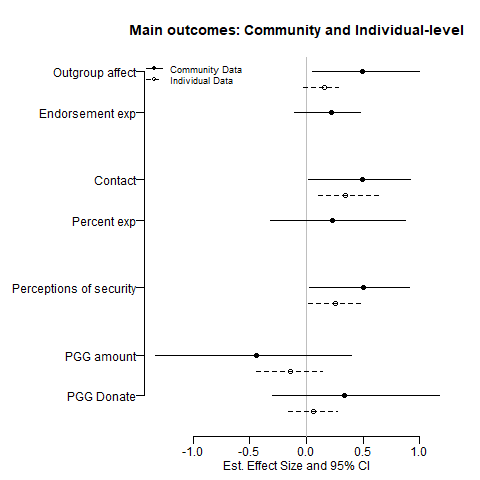
\includegraphics[width=.7\textwidth]{../../../figs/ecpn_coefplots_SurveyOuts-cats.png}
\caption{\label{fig:fig1} \textbf{Effect of treatment assignment on outcomes in community-level and individual-level data.} Points are average treatment effects versus control estimated using OLS. Lines are bootstrapped 95\% confidence intervals.  Solid lines are effects in the community-level data, dashed lines are effects in the individual-level data.  The first set of effects concern intergroup affect; the second set concern voluntary contact; the third concerns security; the last concerns intergroup cooperation.  Effects in the figure are positive if the intervention improved outcomes and negative if it worsened outcomes.}
\end{figure}

Figures \ref{fig:fig1} and \ref{fig:fig2} show the intervention's effect
on the survey and behavioral game outcomes. Figure 1 shows the main
analyses, where the solid lines are the community-level data and the
dashed lines are the individual-level data. Figure 2 shows participants
and nonparticipants compared to controls. From top to bottom, the
outcomes are ordered to correspond with: (1) intergroup affect, (2)
intergroup contact, (3) perceptions of physical security, and (4)
intergroup cooperation. The analysis of survey experiments is only
possible in the community-level analysis.

\begin{figure}[H]
\centering
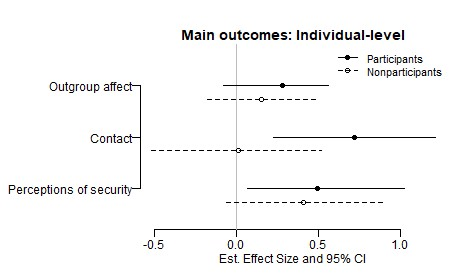
\includegraphics[width=.7\textwidth]{../../../figs/ecpn_coefplots_MainOuts_panel-cats2.jpg}
\caption{\label{fig:fig2} \textbf{Effect of treatment assignment on participants and nonparticipants.} Points are average treatment effects versus control estimated using OLS. Lines are bootstrapped 95\% confidence intervals.  Solid lines are effects among participants, dashed lines are effects among nonparticipants living in treatment communities.  Effects in the figure are positive if the intervention improved outcomes and negative if it worsened outcomes.}
\end{figure}

Figure \ref{fig:obs} shows the intervention's effect on behavior
observed in markets and at social events. From top to bottom, the
outcomes are ordered to correspond with: (1) the number of pastoralist
buyers and sellers in markets , (2) the number of farmer buyers and
sellers in markets, (3) attendance from each group at social events
hosted by the other, and (4) food eating by each group at social events
hosted by the other. These analysese are only possible at the community
level because we did not identify specific individuals at social events
or in markets.

\begin{figure}[H]
\centering
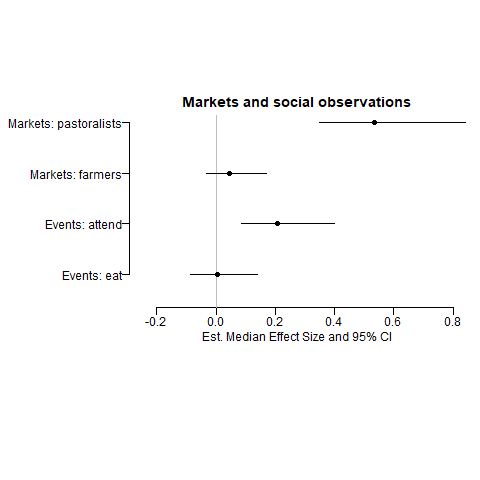
\includegraphics[width=.7\textwidth]{../../../figs/ecpn_coefplots_markEvents.png}
\vspace{-1cm}
\caption{\label{fig:obs} \textbf{Effect of treatment assignment on behavior in markets and at social events.} Points are average treatment effects versus control estimated using quantile regression. Lines are 95\% confidence intervals.  Effects in the figure are positive if the intervention improved outcomes and negative if it worsened outcomes.}
\end{figure}

\hypertarget{intergroup-affect}{%
\subsection{Intergroup Affect}\label{intergroup-affect}}

The intervention bolstered intergroup affect in treatment communities.
Compared to control communities, respondents in treatment communities
report more trust in the other group and are more comfortable engaging
in various relationships with the outgroup, such as trading goods and
intermarriage. Intergroup affect as measured by the endorsement
experiment also improves more in the treatment group than the control
group, though the difference is not statistically significant at
conventional levels.

\begin{figure}[H]
    \begin{subfigure}[b]{.48\textwidth}
    \centering
        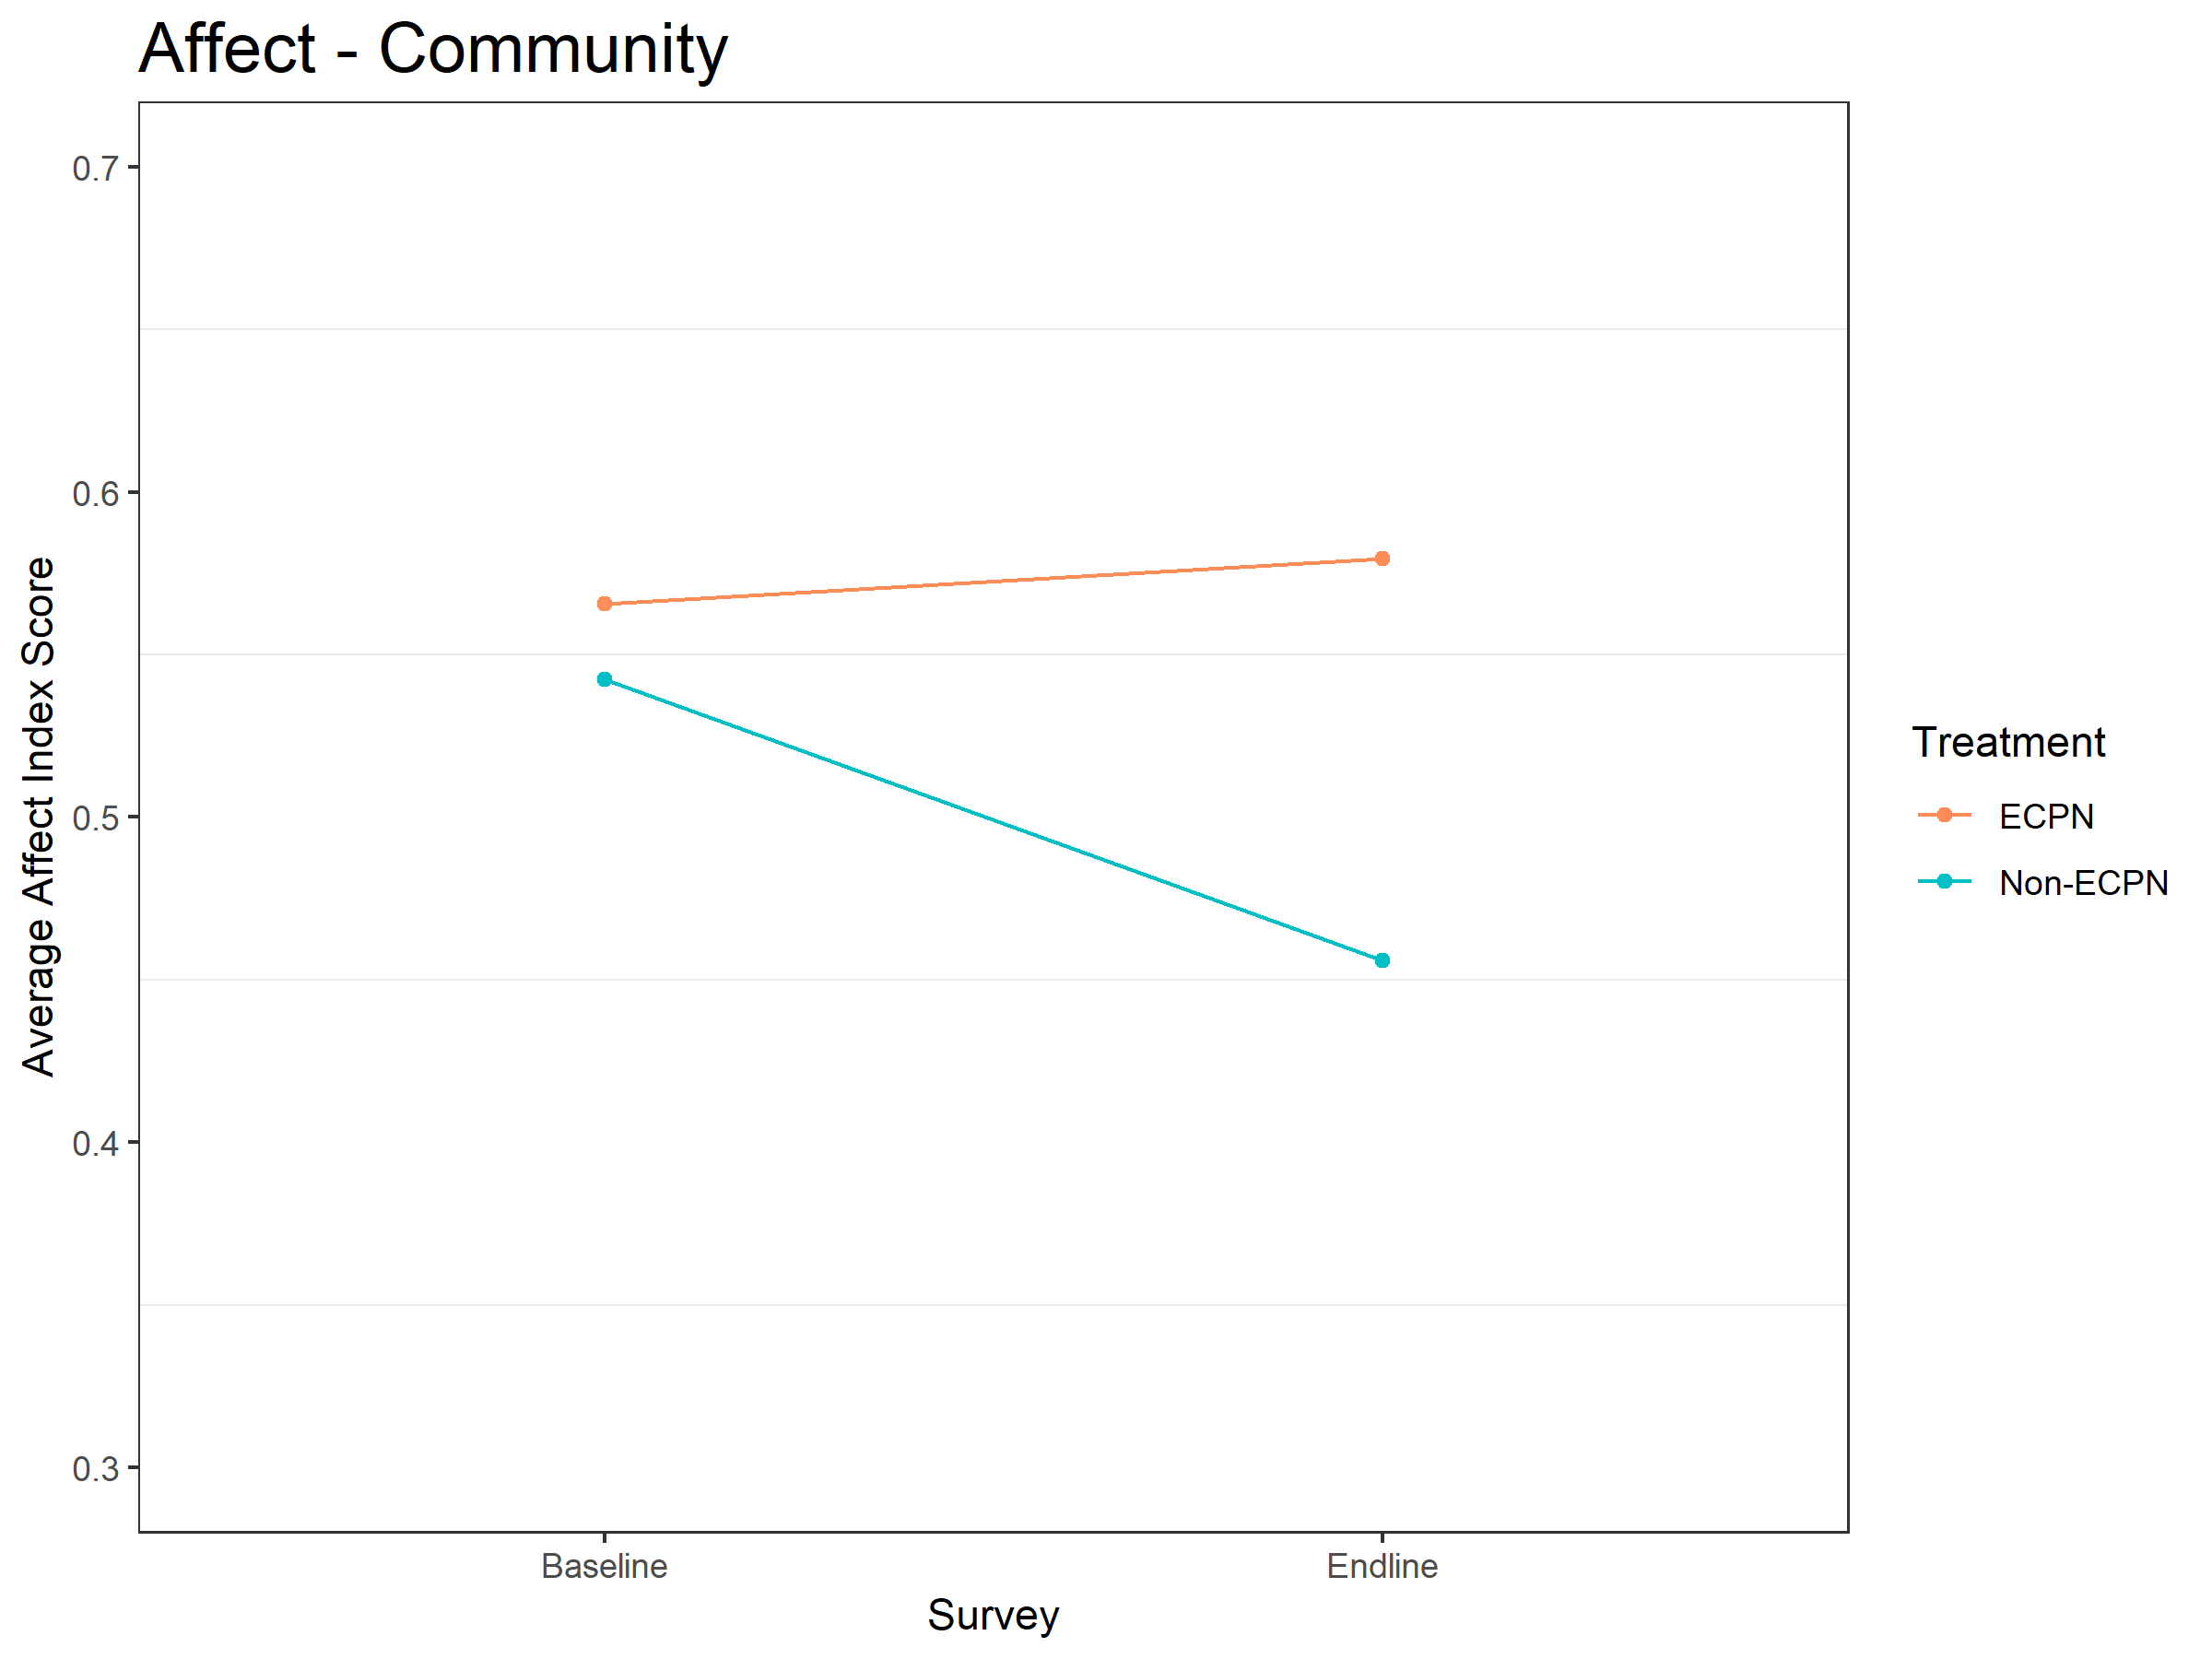
\includegraphics[width=\linewidth]{../../../figs/affectComm_plot.png}
        \caption{\textbf{Descriptive change in community-level intergroup affect from baseline to endline.} Red line is treatment site average, blue line is control site average.}
        \label{fig:fig3}
    \end{subfigure}
    \hfill
    \begin{subfigure}[b]{.48\textwidth}
    \centering
        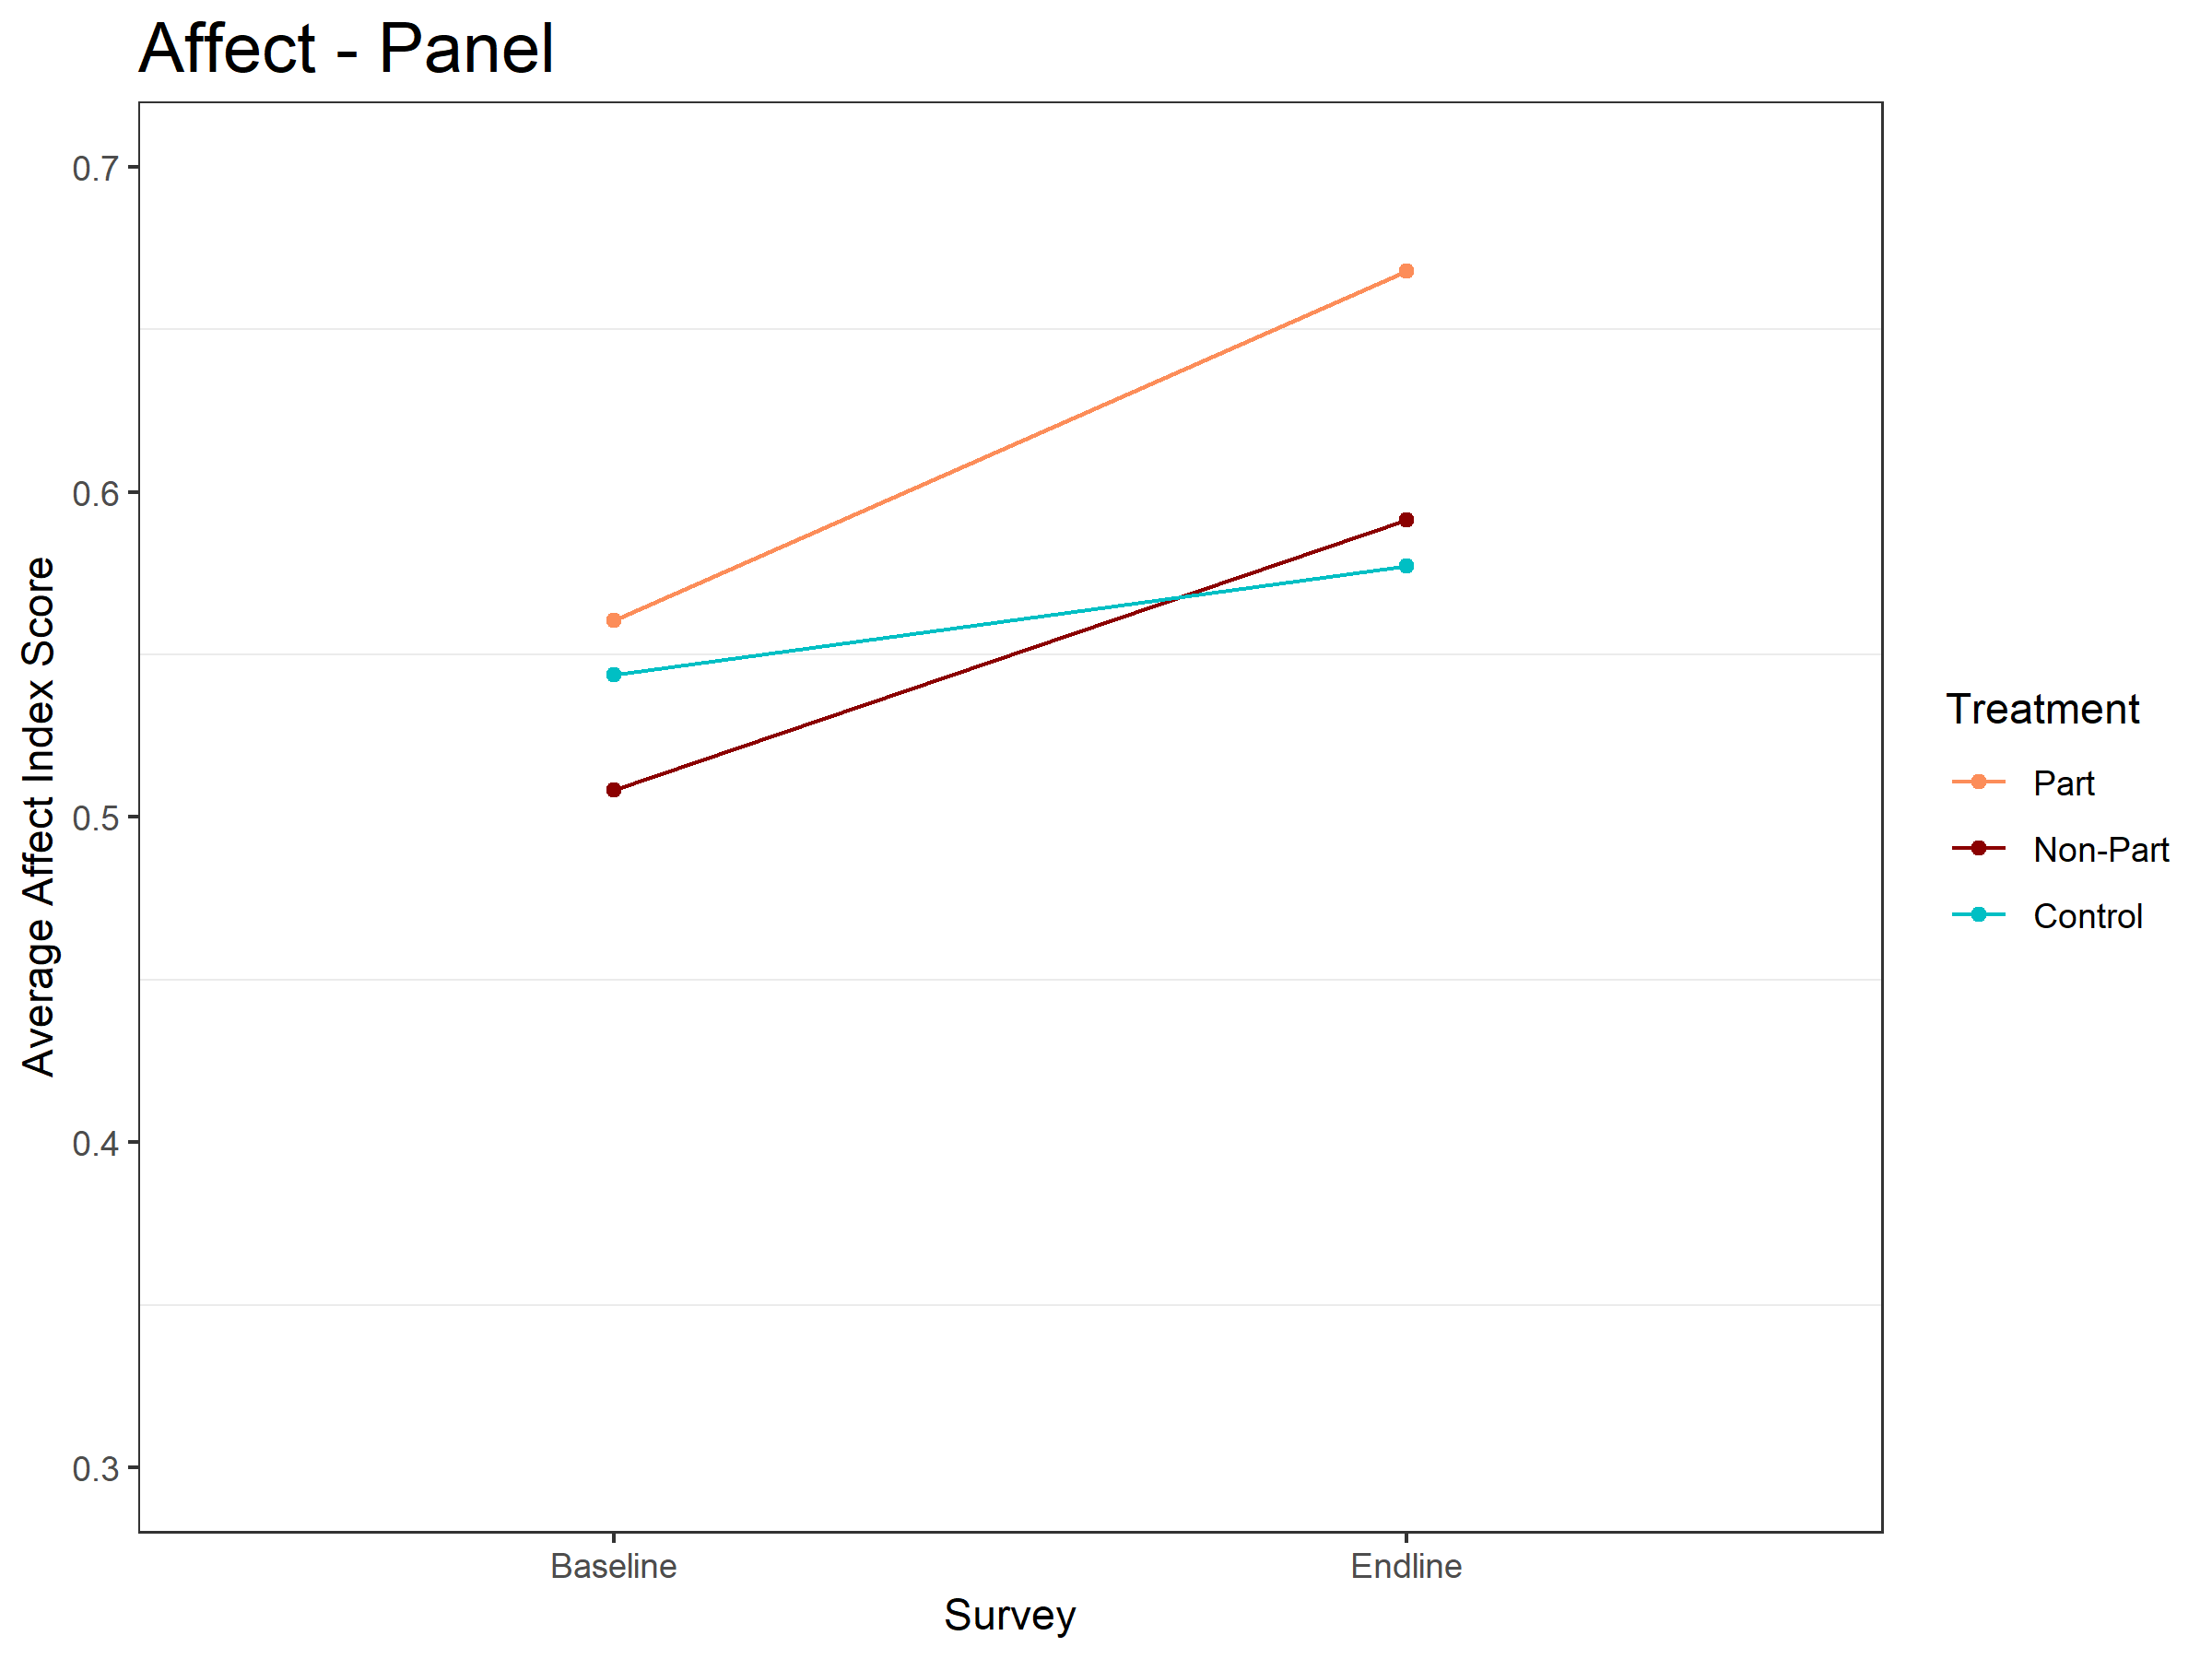
\includegraphics[width=\linewidth]{../../../figs/affectPan_plot.png}
        \caption{\textbf{Descriptive change in individual-level intergroup affect from baseline to endline.} Red line is participant average, dark red line is nonparticipant average, blue line is control average.}
        \label{fig:fig4}
    \end{subfigure}
\caption{\textbf{Intergroup Affect.} Moving up the Y-axis indicates improved affect between groups.}
\end{figure}

Figures \ref{fig:fig3} and \ref{fig:fig4} show the descriptive change in
affect for treatment and control communities. Affect in control
communities decreased from baseline to endline, while intervention
communities improved over the same time period. As measured by the
endorsement experiment, affect declines in both treatment and control
communities, but declines more in control communities. Both measures
suggest that the intervention improved affect towards the outgroup.

\hypertarget{perceptions-of-physical-security}{%
\subsection{Perceptions of Physical
Security}\label{perceptions-of-physical-security}}

The intervention substantially increased feelings of security in the
treatment group. The effect is large in both the community-level and the
individual-level data. Perceptions of physical security in treatment
communities improved far more from baseline to endline than in control
communities. At the individual-level, participants and nonparticipants
improved equally, suggesting that these increases reflect a change in
the conflict environment that impacts the entire community, not just
respondents involved in ECPN committees. These improvements in treatment
communities are especially powerful because other survey questions show
that the intervention increased awareness of the conflict -- respondents
in treatment communities are more likely than the control to know that
violence between groups has occurred recently, yet they feel more
secure.

\begin{figure}[H]
    \begin{subfigure}[b]{.48\textwidth}
    \centering
        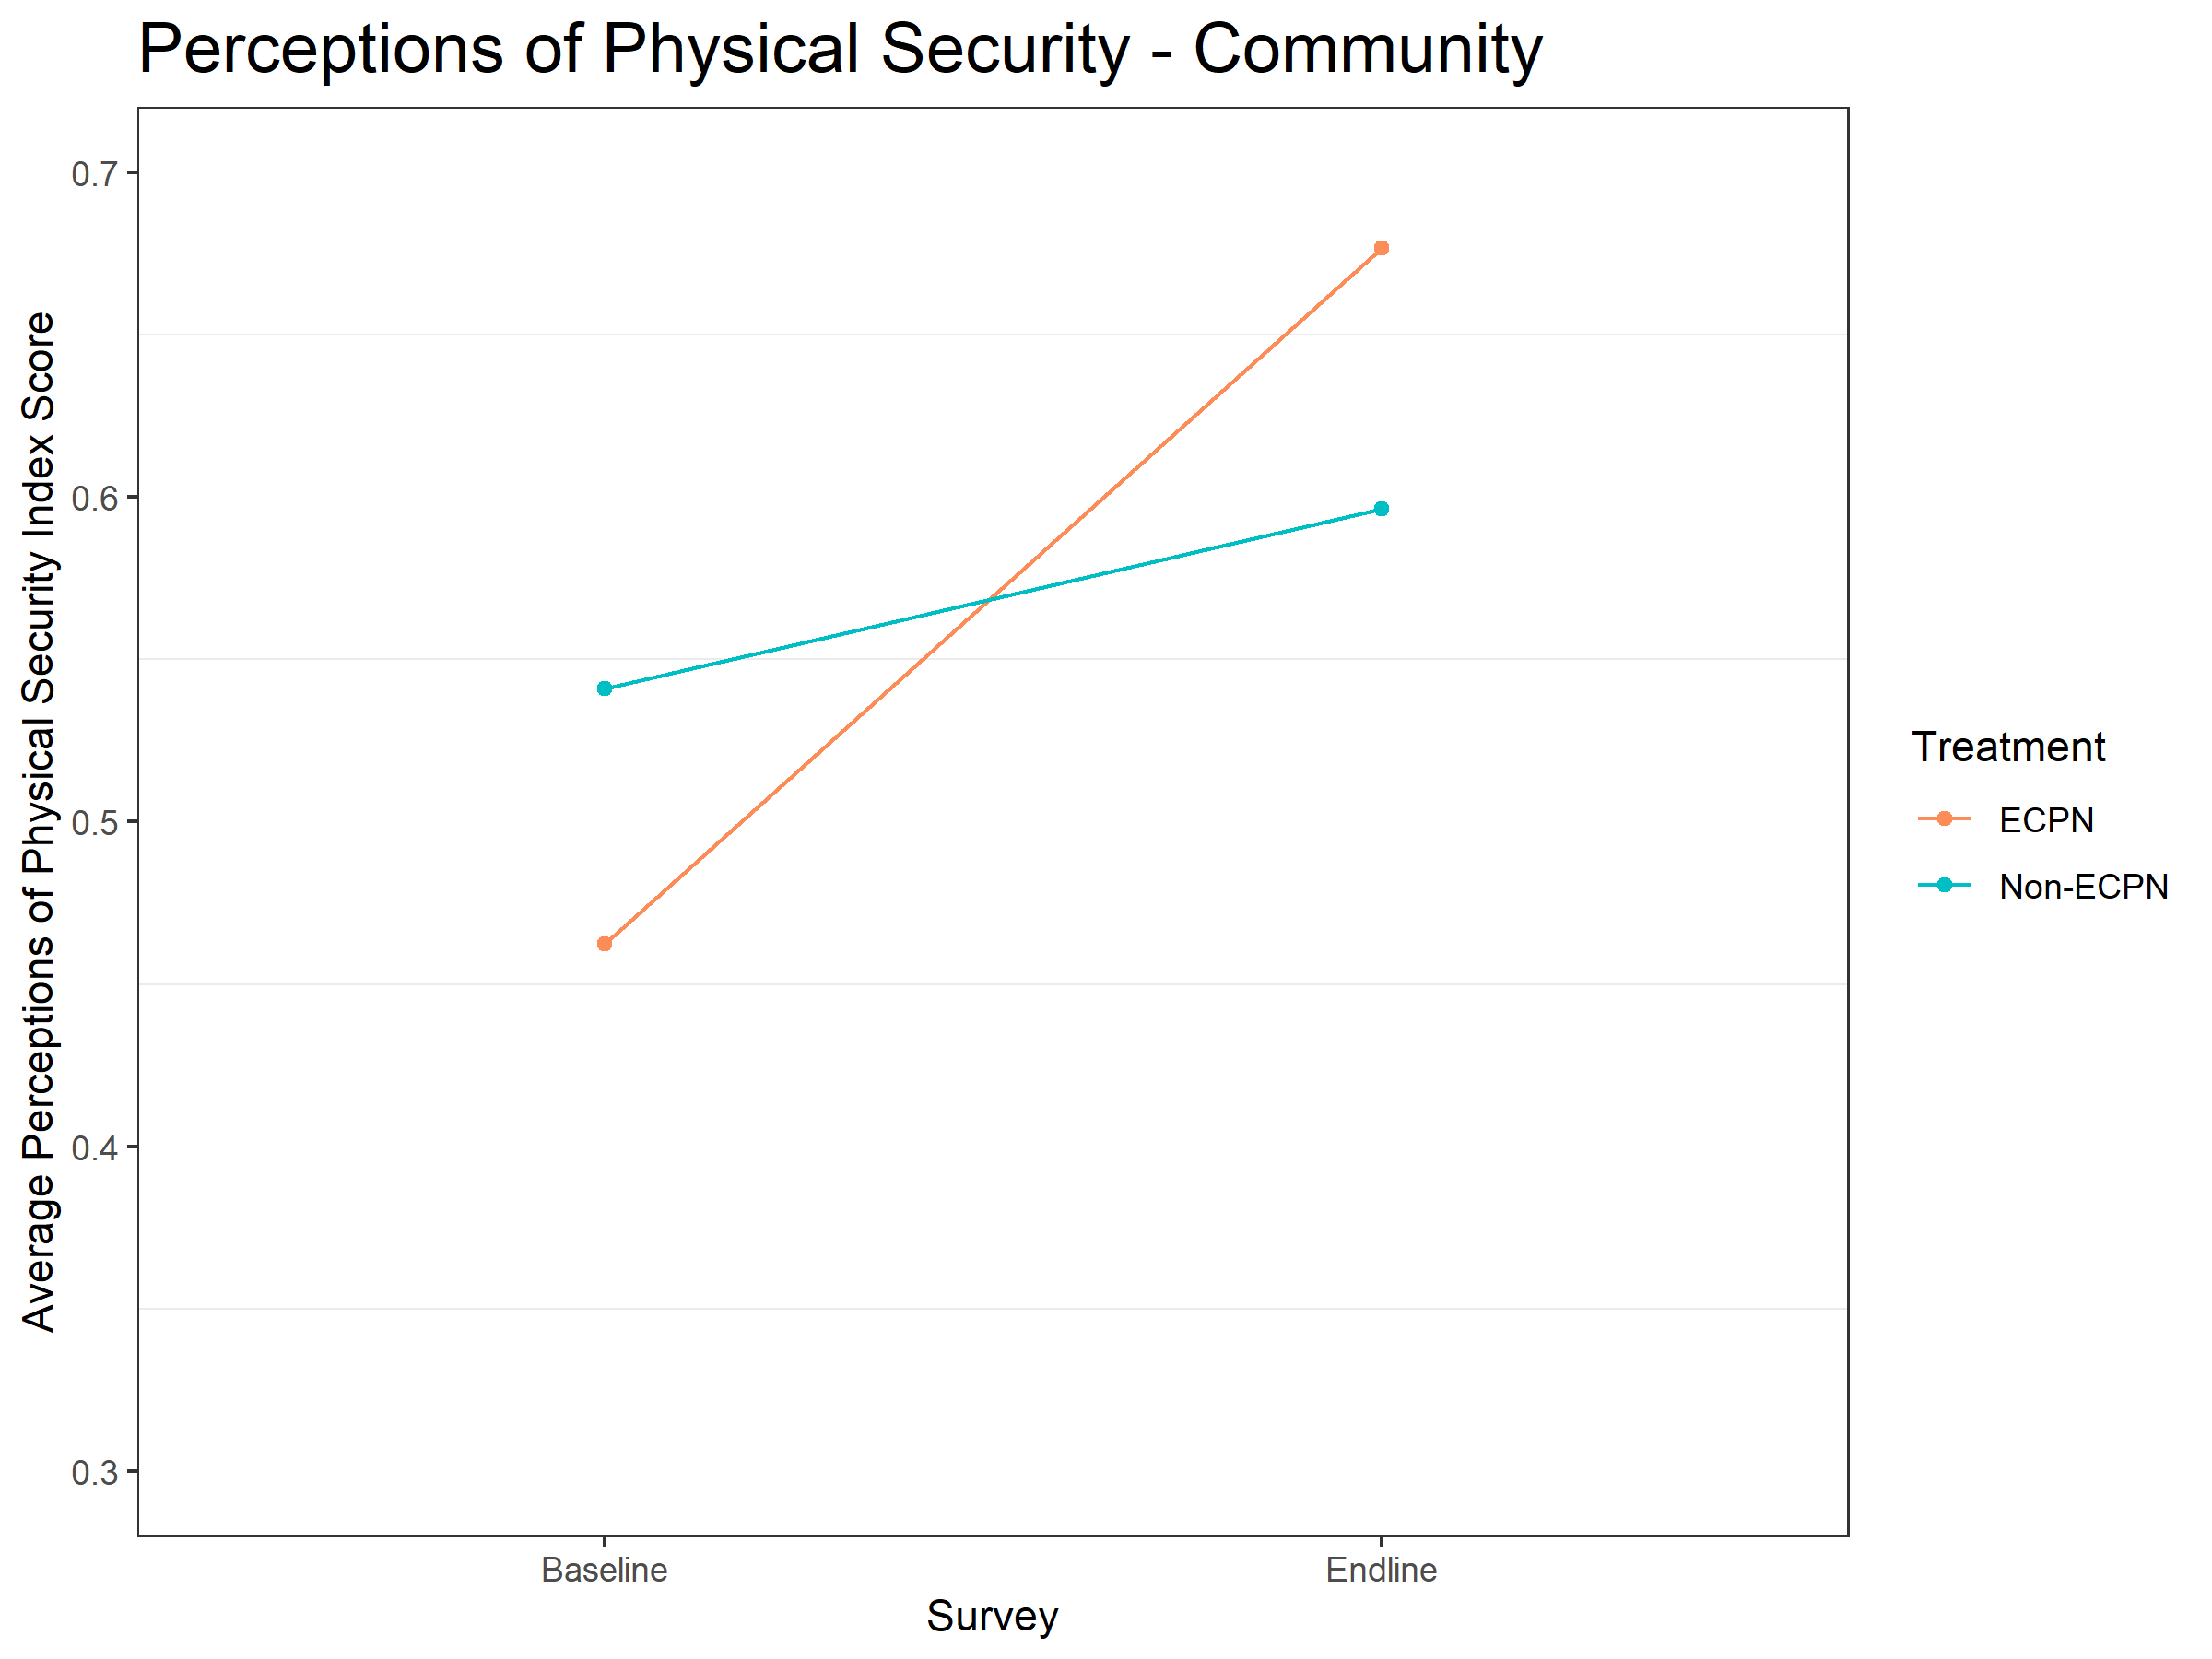
\includegraphics[width=\linewidth]{../../../figs/inComm_plot.png}
        \caption{\textbf{Descriptive change in community-level insecurity from baseline to endline.} Red line is treatment site average, blue line is control site average.}
        \label{fig:fig7}
    \end{subfigure}
    \hfill
    \begin{subfigure}[b]{.48\textwidth}
    \centering
        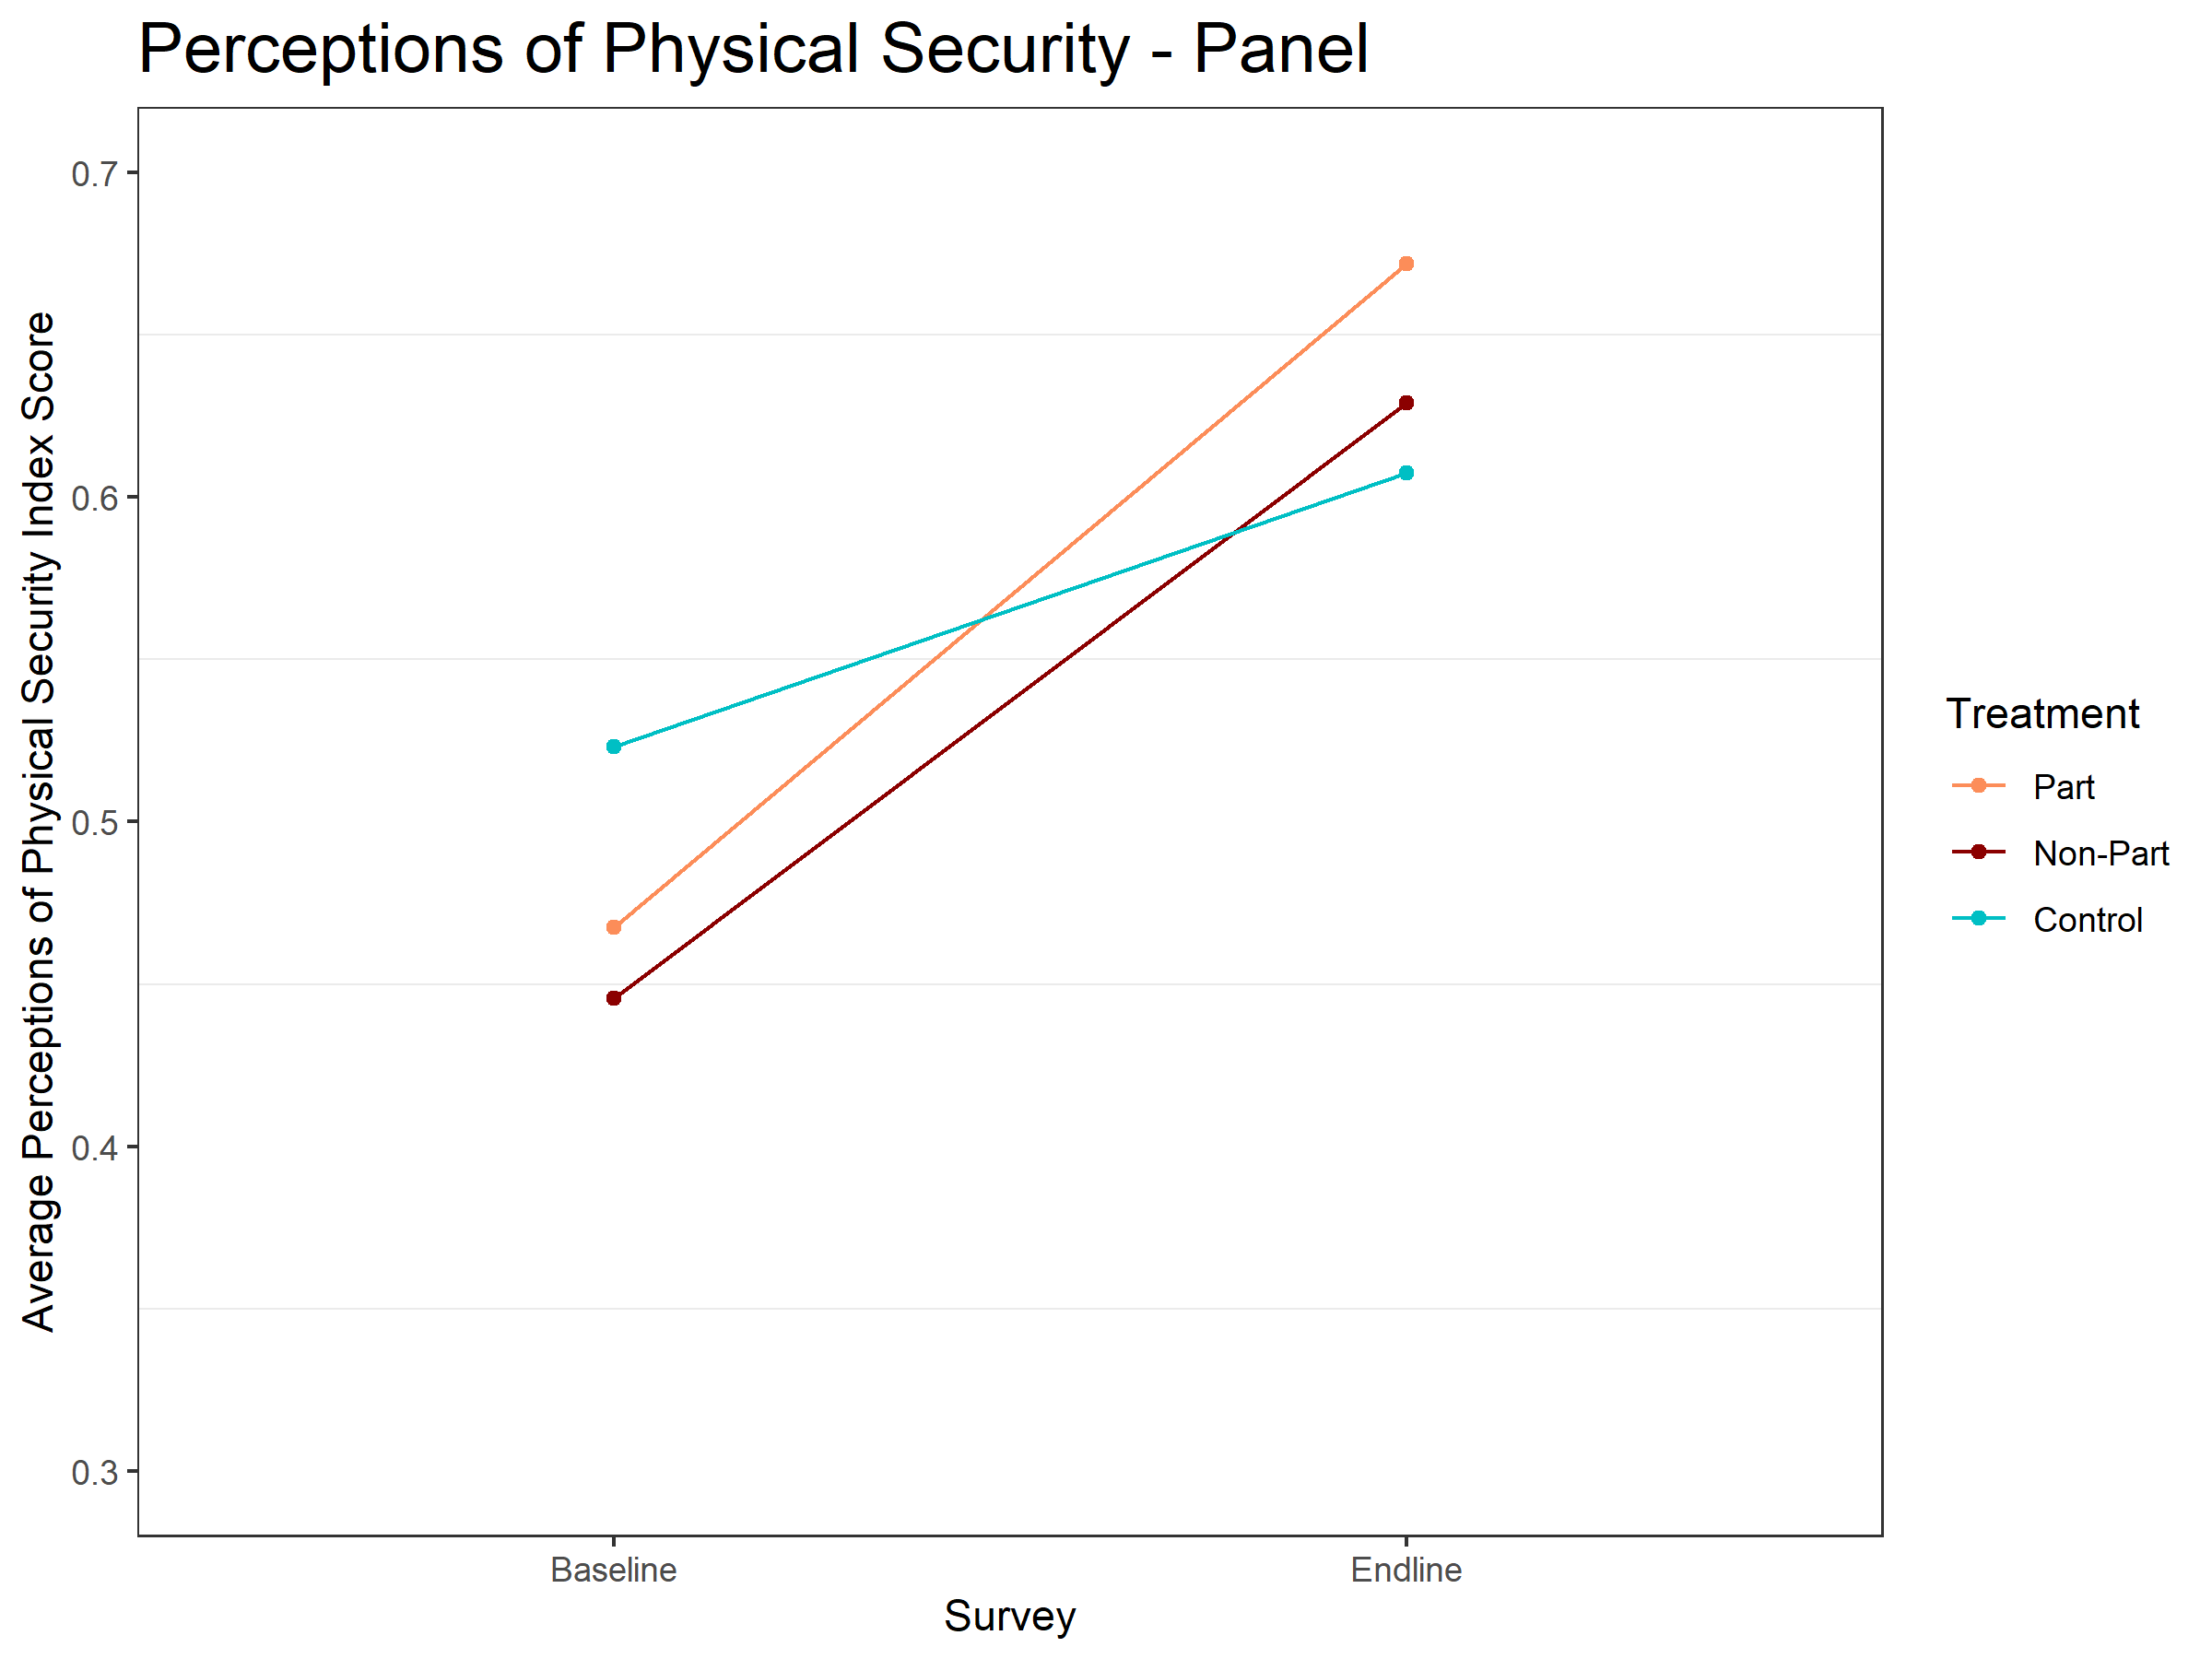
\includegraphics[width=\linewidth]{../../../figs/inPan_plot.png}
        \caption{\textbf{Descriptive change in individual-level insecurity from baseline to endline.} Red line is participant average, dark red line is nonparticipant average, blue line is control average.}
        \label{fig:fig8}
    \end{subfigure}
    \caption{\textbf{Perceptions of Physical Security.}  Moving up the Y-axis indicates improved security.}
\end{figure}

Figures \ref{fig:fig7} and \ref{fig:fig8} show the descriptive change in
perceptions of physical security for treatment and control communities.
The security perceptions of control communities improved slightly from
baseline to endline but security perceptions in treatment communities
improved substantially more over that same period. Treatment communities
initially felt less secure than control communities but felt more secure
at the end of the program.

\hypertarget{contact}{%
\subsection{Contact}\label{contact}}

The effect of the intervention on contact is substantial. Respondents in
treatment communities report more contact and more willingness to engage
in contact at all levels of the percent experiment; we also observe more
pastoralists in markets interacting with farmers. Since the markets are
all located in the farming community, the sustained presence of
pastoralists there suggests that (1) farmers were accepting/tolerant of
pastoralists in their community and (2) pastoralists felt comfortable
spending time in the farmer community. The number of farmers present in
the markets does not change in either group, which makes sense because
the market is inside the farming community.

\begin{figure}[H]
    \begin{subfigure}[b]{.48\textwidth}
    \centering
        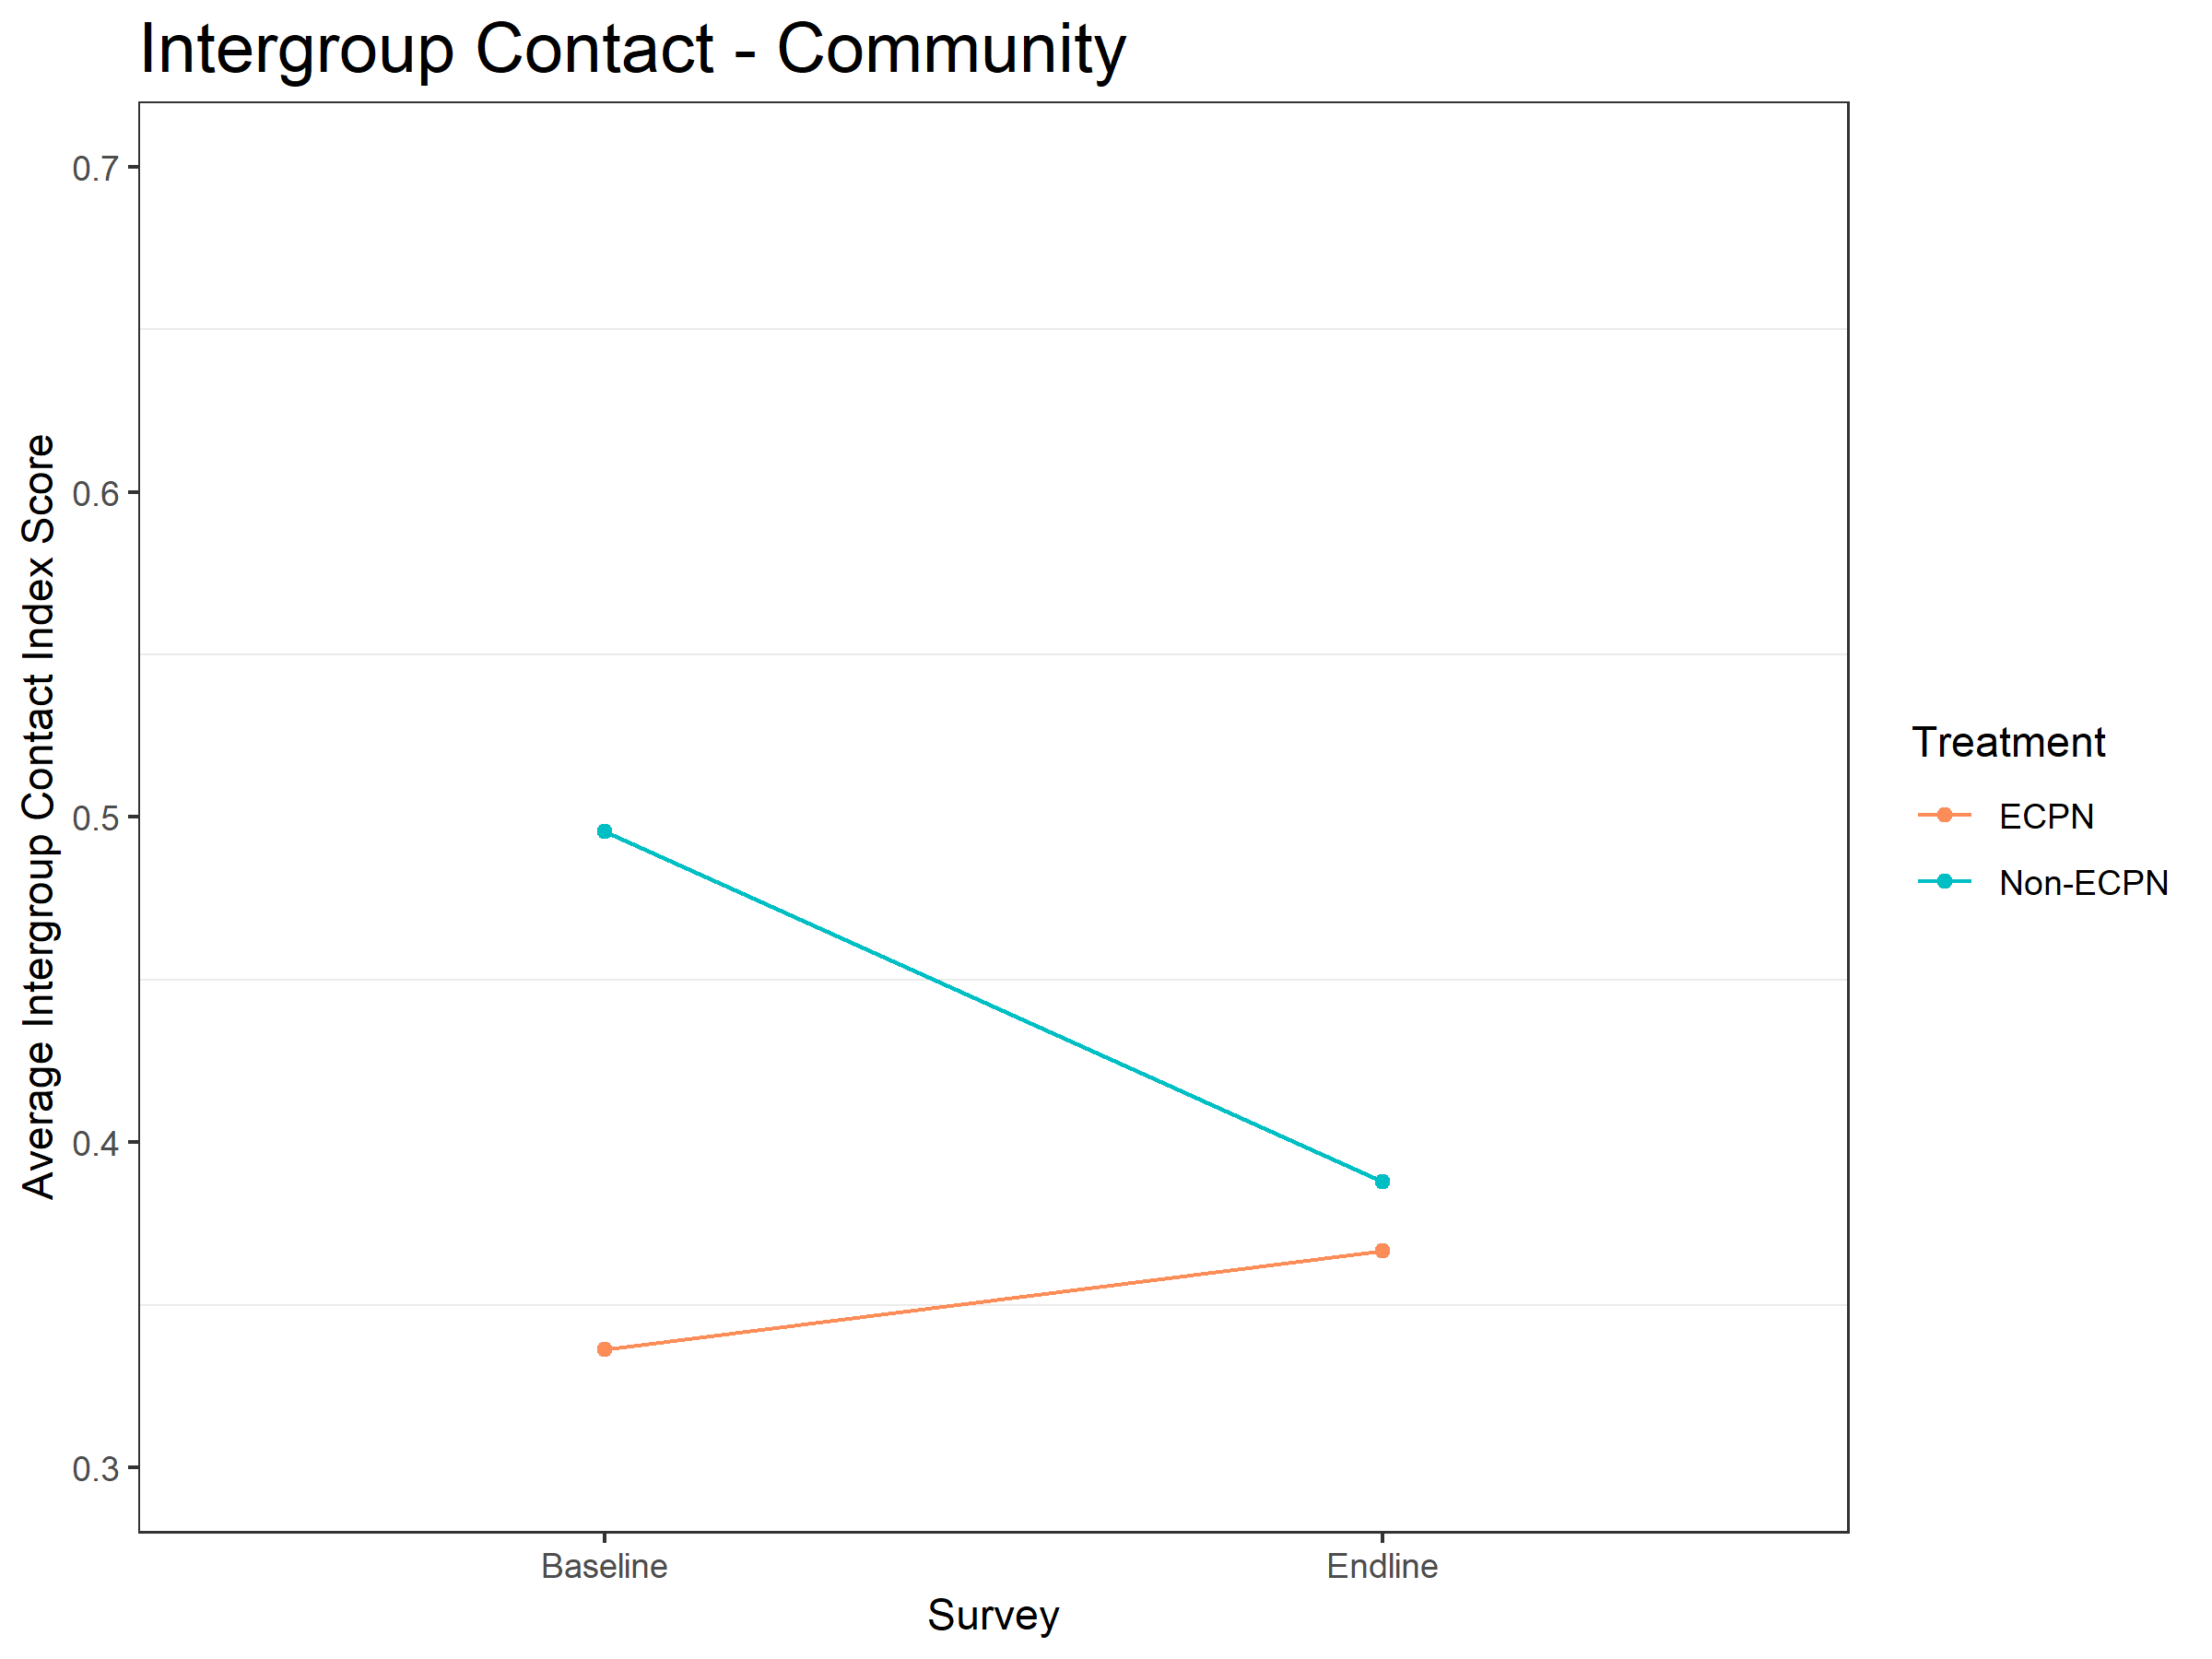
\includegraphics[width=\linewidth]{../../../figs/conComm_plot.png}
        \caption{\textbf{Descriptive change in community-level voluntary contact from baseline to endline.} Red line is treatment site average, blue line is control site average.}
        \label{fig:fig5}
    \end{subfigure}
    \hfill
    \begin{subfigure}[b]{.48\textwidth}
    \centering
        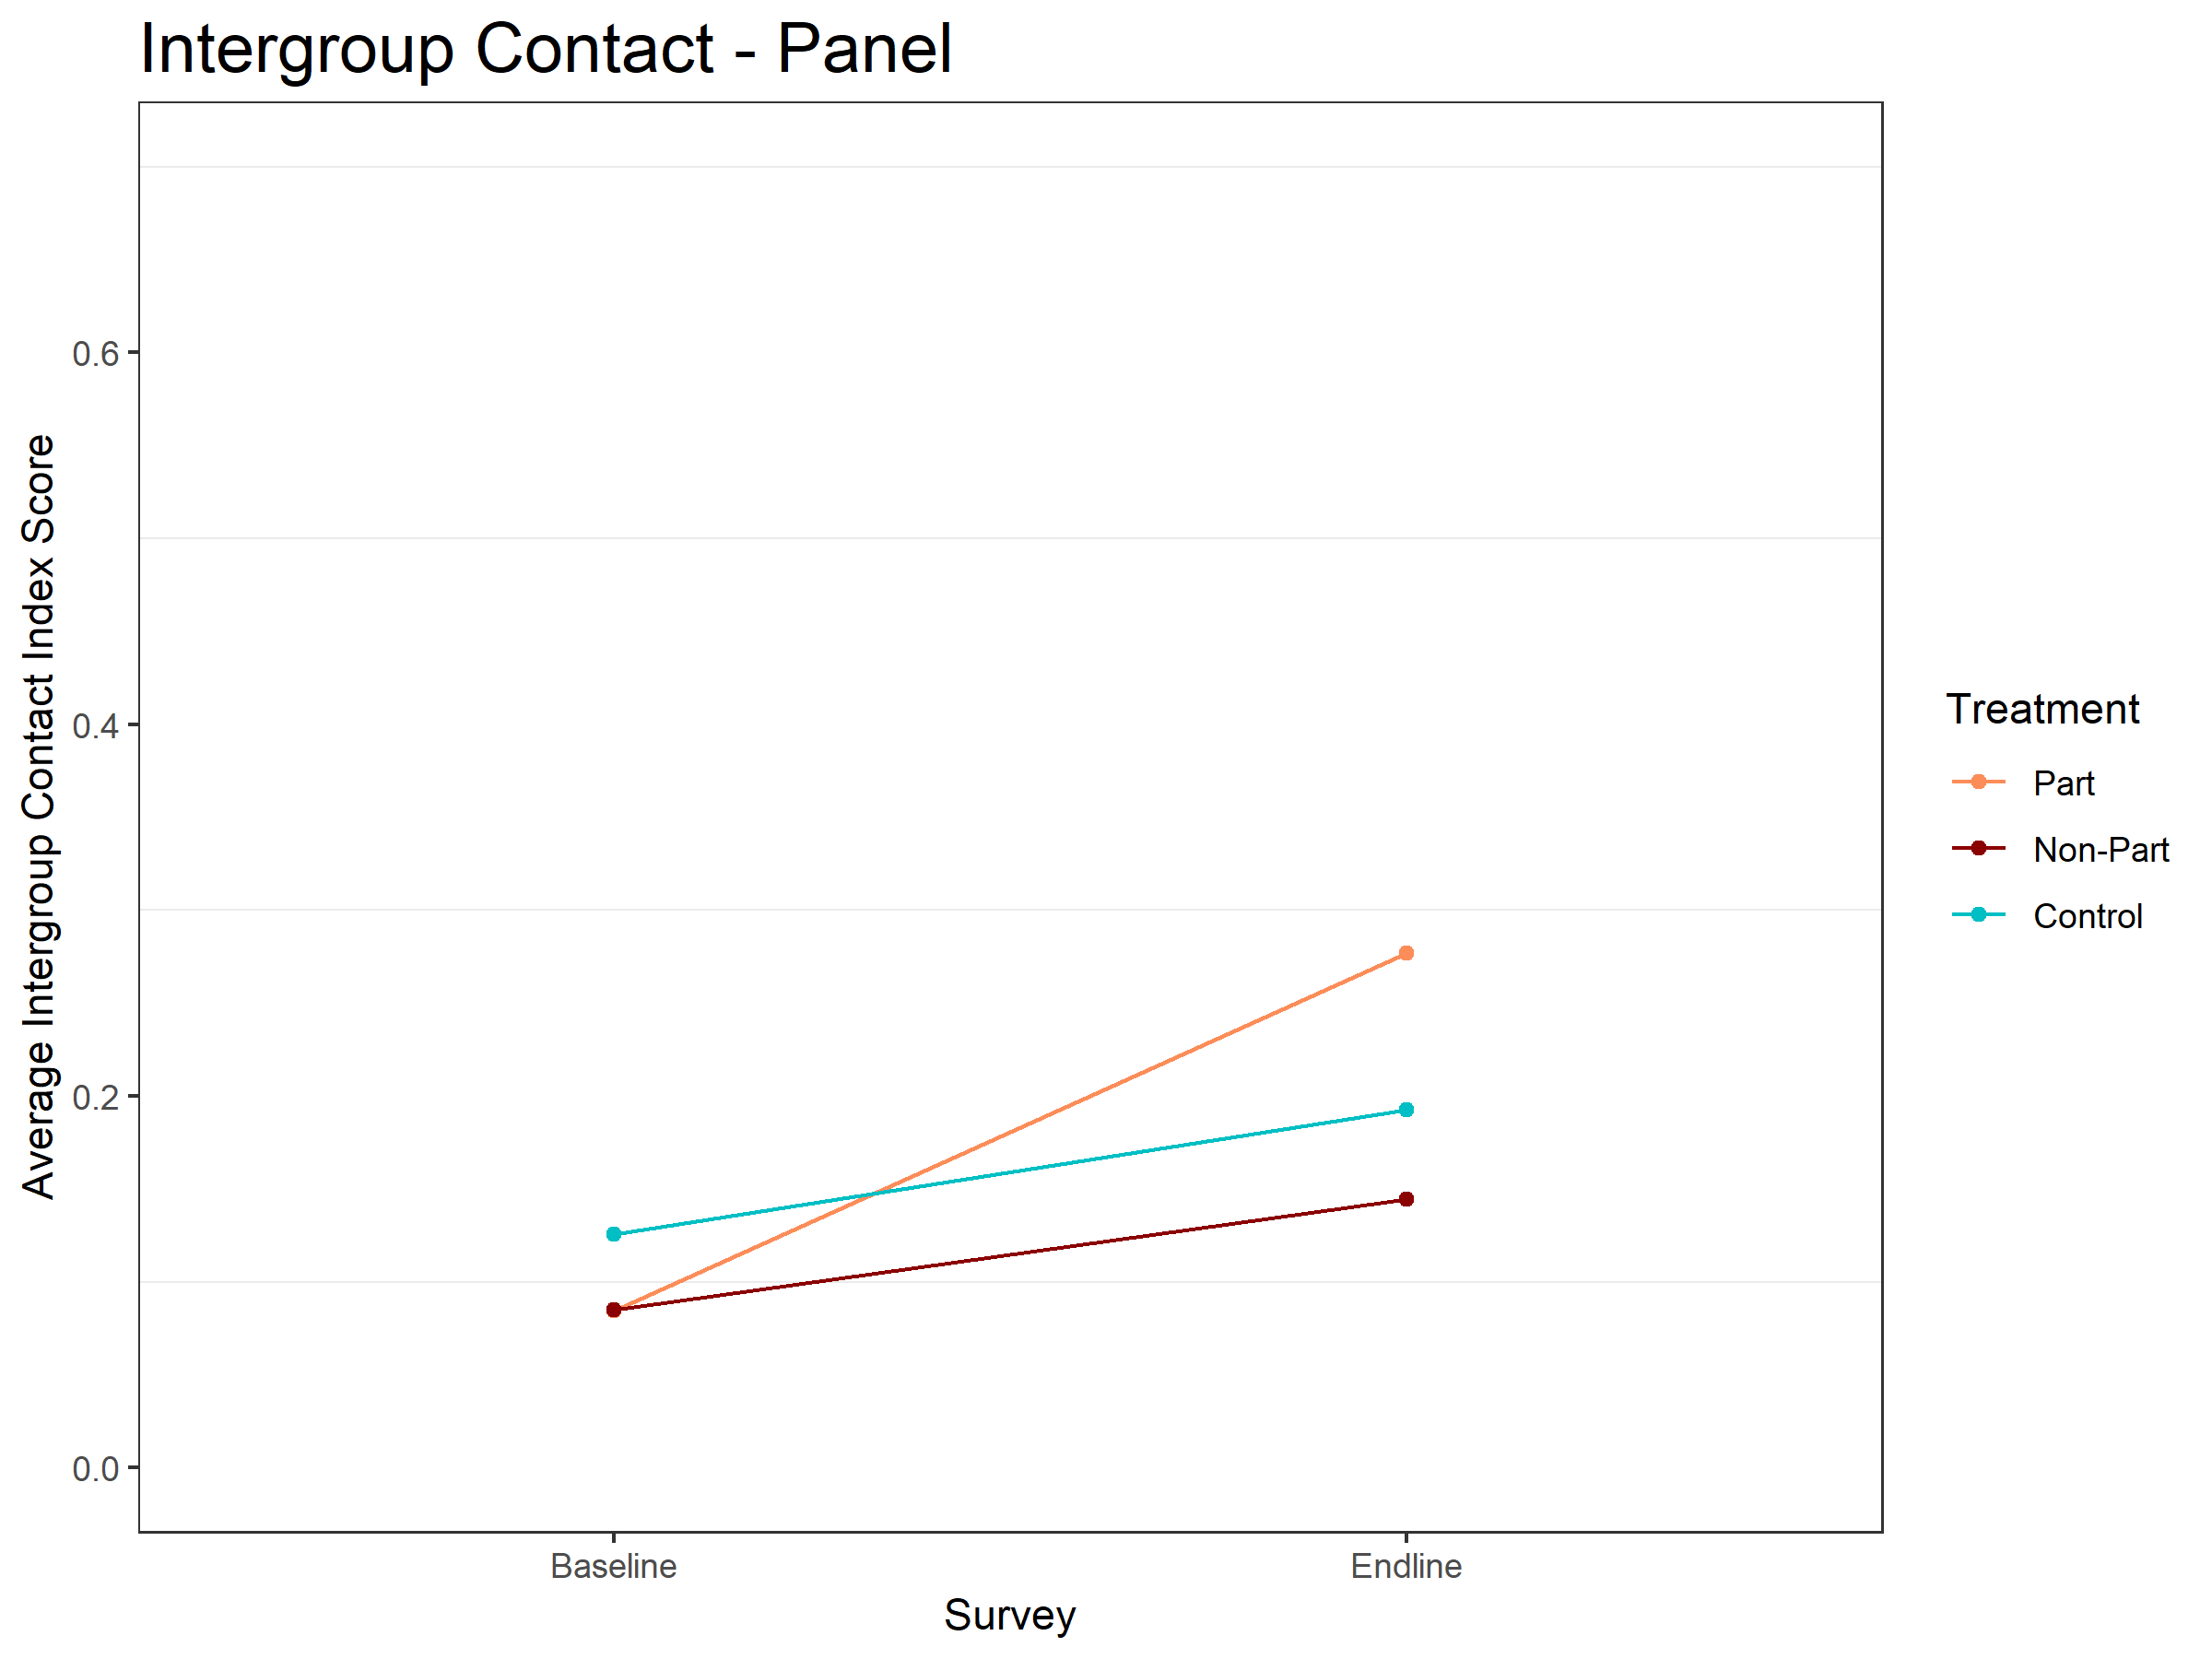
\includegraphics[width=\linewidth]{../../../figs/conPan_plot.png}
        \caption{\textbf{Descriptive change in individual-level voluntary contact from baseline to endline.} Red line is participant average, dark red line is nonparticipant average, blue line is control average.}
        \label{fig:fig6}
    \end{subfigure}
    \caption{\textbf{Voluntary Contact.}  Moving up the Y-axis indicates improved contact between groups.}
\end{figure}

Figures \ref{fig:fig5} and \ref{fig:fig6} show the descriptive change in
contact for treatment and control communities. The community-level
self-reports show that intergroup contact declined sharply in control
communities but rose slightly in treatment communities. The intervention
was able to increase contact even as the social environment led to a
sharp decline in control sites. At the individual-level, intergroup
contact increased at the same rate for nonparticipants and controls but
increased a great deal more for committee participants. This parallel
relationship for nonparticipants and controls contradicts the large
community-level effect, which suggested that the effects of the
intervention extend to nonparticipants in treatment communities. One
plausible explanation is that the effect on nonparticipants did not
extend to the type of nonparticipant we could track down and resurvey;
another explanation is that the type of control individual we could
track down for resurveying increased their intergroup contact even as
the rest of the community decreased theirs.

\hypertarget{intergroup-cooperation}{%
\subsection{Intergroup Cooperation}\label{intergroup-cooperation}}

The results of the PGG suggest that the intervention did not affect
respondents' capacity to cooperate with the outgroup. Figures
\ref{fig:pggComm} and \ref{fig:pggPan} show the descriptive difference
in the proportion of respondents who donated and average donation amount
for treatment and control communities at endline. Respondents in
treatment communities were slightly more likely to donate any amount,
but had a lower average donation than control communities. In the
individual-level data, participants and nonparticipants in treatment
communities were also slightly more likely to donate any amount than
controls, but the average donation amount is highest among controls and
lowest among ECPN participants.

\begin{figure}[H]
    \begin{subfigure}[b]{.48\textwidth}
    \centering
        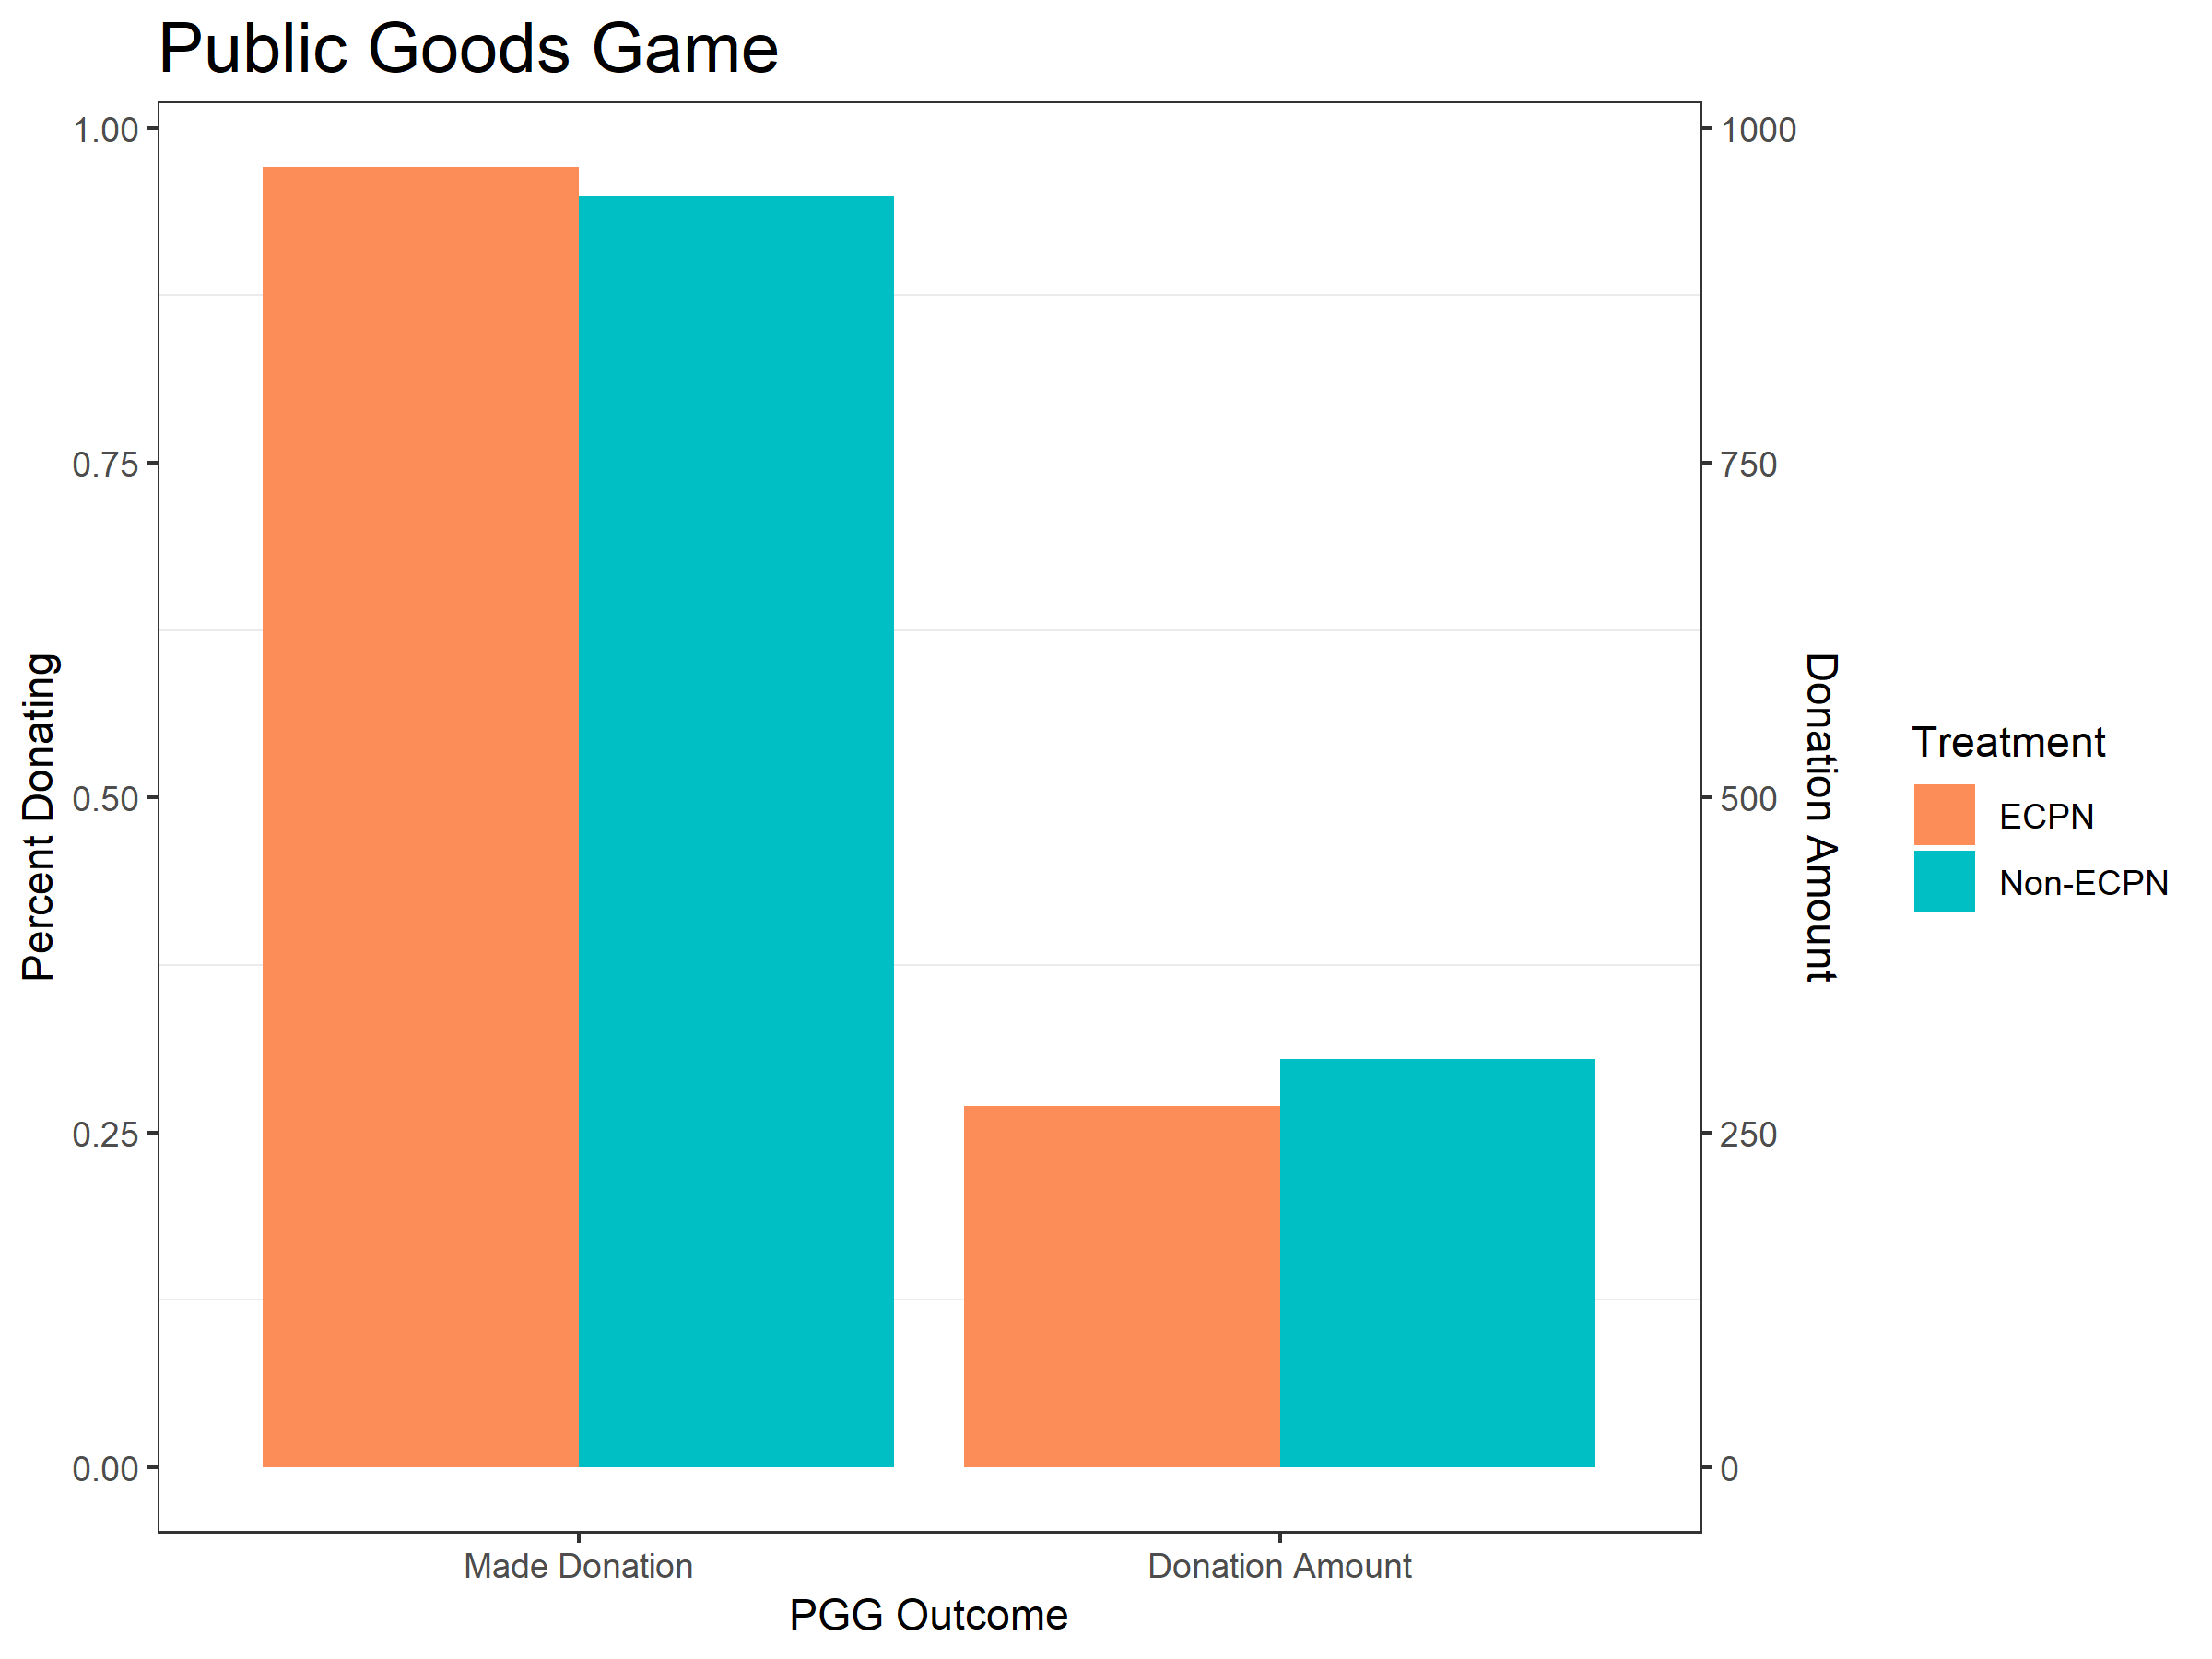
\includegraphics[width=\linewidth]{../../../figs/pggComm_plot.png}
        \caption{\textbf{Descriptive difference in community-level donations to a public good at endline.} Red bar is treatment site average, blue bar is control site average.}
        \label{fig:pggComm}
    \end{subfigure}
    \hfill
    \begin{subfigure}[b]{.48\textwidth}
    \centering
        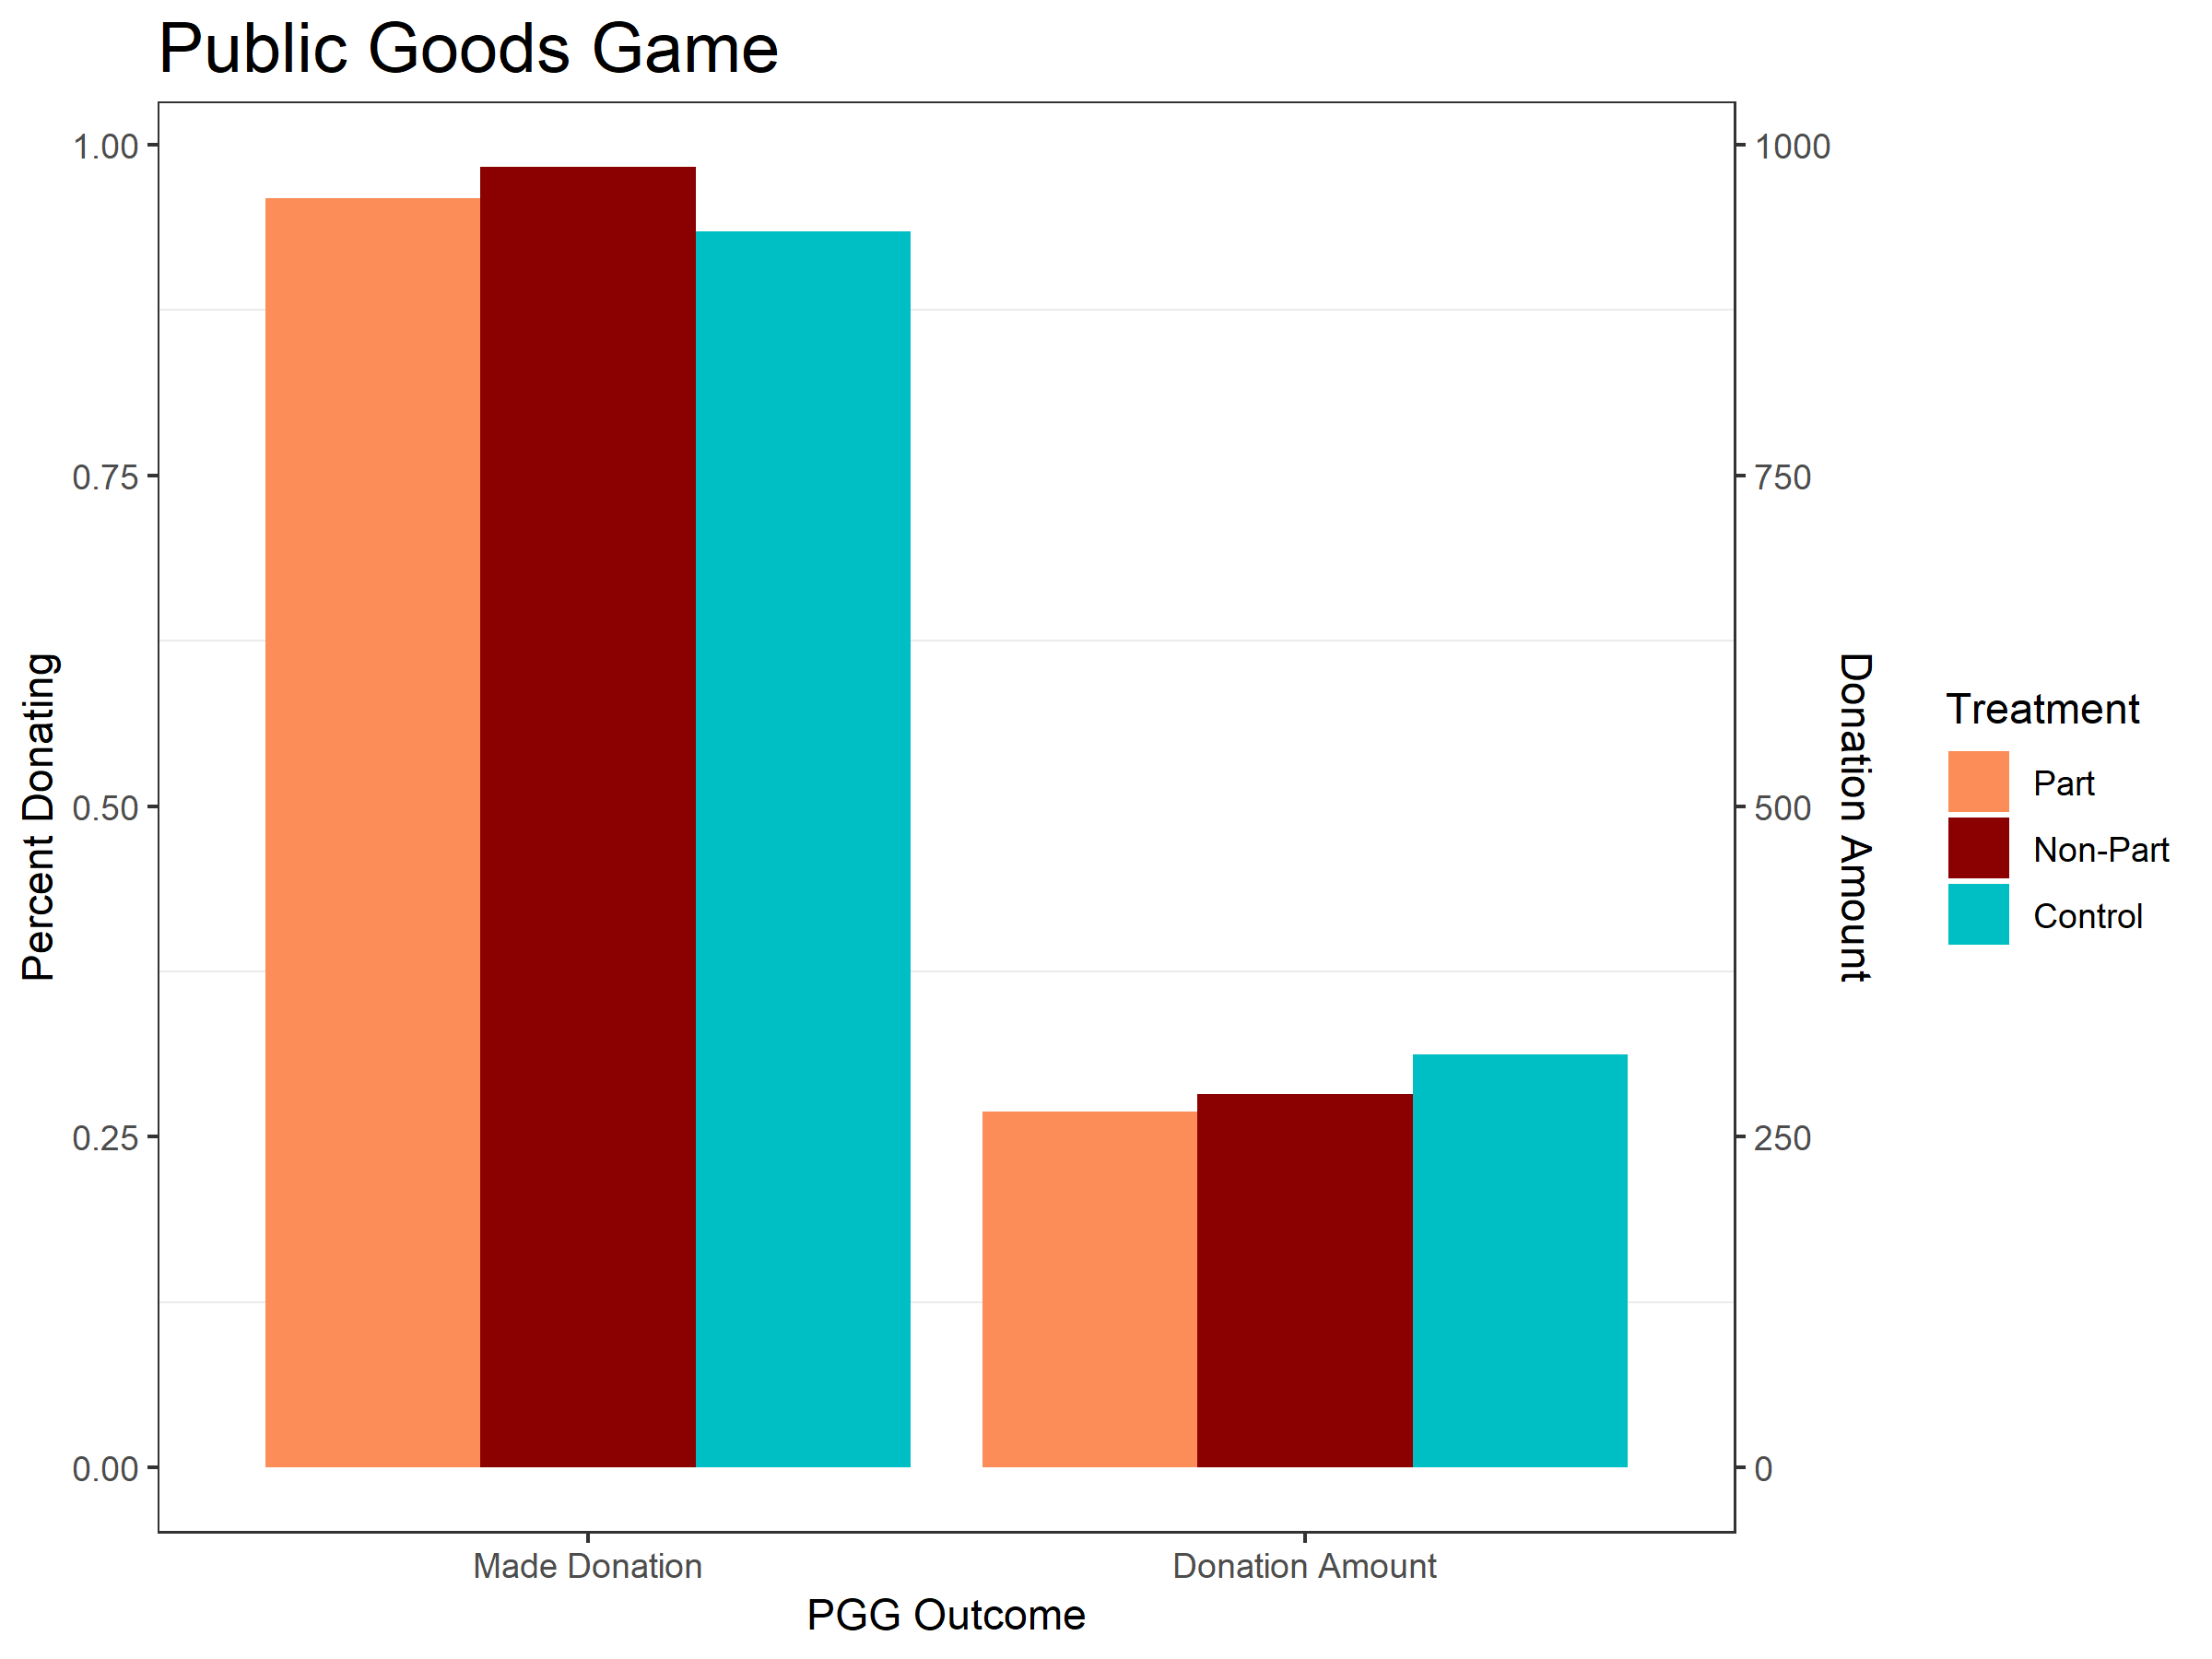
\includegraphics[width=\linewidth]{../../../figs/pggPan_plot.png}
        \caption{\textbf{Descriptive difference in individual-level donations to a public good at endline.} Red bar is participant average, dark red bar is nonparticipant average, blue bar is control average.}
        \label{fig:pggPan}
    \end{subfigure}
    \caption{\textbf{Donations in public goods game.}  Moving up the Y-axis indicates a greater percentage of respondents donating and a higher average donation amount.}
\end{figure}

Our fieldwork suggests that the public goods game was not an effective
measure of intergroup cooperation in this instance. For example, a
control community raised the most money, with respondents donating over
half of the PGG money to the community fund. Without context, the data
says that this community is highly cooperative. However, the divisions
in this community were so problematic that the farmers and pastoralists
could not agree on who would hold the money they raised. The community
fund had to be held at Mercy Corps' Abuja office until the communities
decided how to spend the money. This and other experiences indicate that
donations were not primarily motivated by feelings towards the outgroup
and were more likely motivated by ingroup norms and the possibility of
proving to Mercy Corps that their community was a good community to run
a program.

\hypertarget{exploring-these-effects-state-level-differences}{%
\subsection{Exploring these effects: state-level
differences}\label{exploring-these-effects-state-level-differences}}

We note that some of our findings are due to outcomes worsening in
control sites rather than improving in treatment sites. To understand
these trends in greater depth, we explored state-level differences. We
chose to look at state-level differences because Benue experienced an
exogenous shock before the endline survey that may explain worsening
outcomes in the control group. Benue, which always suffered more violent
conflict than Nassarawa, enacted an anti-grazing law making it illegal
for pastoralists to graze animals outside of fenced in areas. This law
led to violence and a migration of pastoralists out of Benue and into
surrounding states, like Nassarawa.\footnote{The violence in Benue drove
  some of our treatment and control communities out of their traditional
  settlements. We describe the steps we took to survey those communities
  in the appendix.} State-level differences in the effectiveness of the
intervention tell us about the effects in these differing contexts. This
study is not powered to detect statistical differences between treatment
and control groups within Nassarawa and Benue, but we can look
descriptively at differences between treatment and control group's
within each state.

\textbf{Affect}: The overall analysis above suggested that the
intervention increased intergroup affect despite a strongly negative
secular trend. Figures \ref{fig:affect_nas} and \ref{fig:affect_ben}
show baseline-endline changes for intergroup affect in Nassarawa and
Benue, respectively. Disaggregating by state, we see that affect
improved in treatment sites relative to control sites in both states.
The overall secular trend is due to the sharp decline in Benue, where
affect fell sharply in control sites while declining only slightly in
treatment sites. In Nassarawa, affect improved modestly in both types of
sites and increased most in treatment sites.

\begin{figure}[H]
    \begin{subfigure}[b]{.48\textwidth}
    \centering
        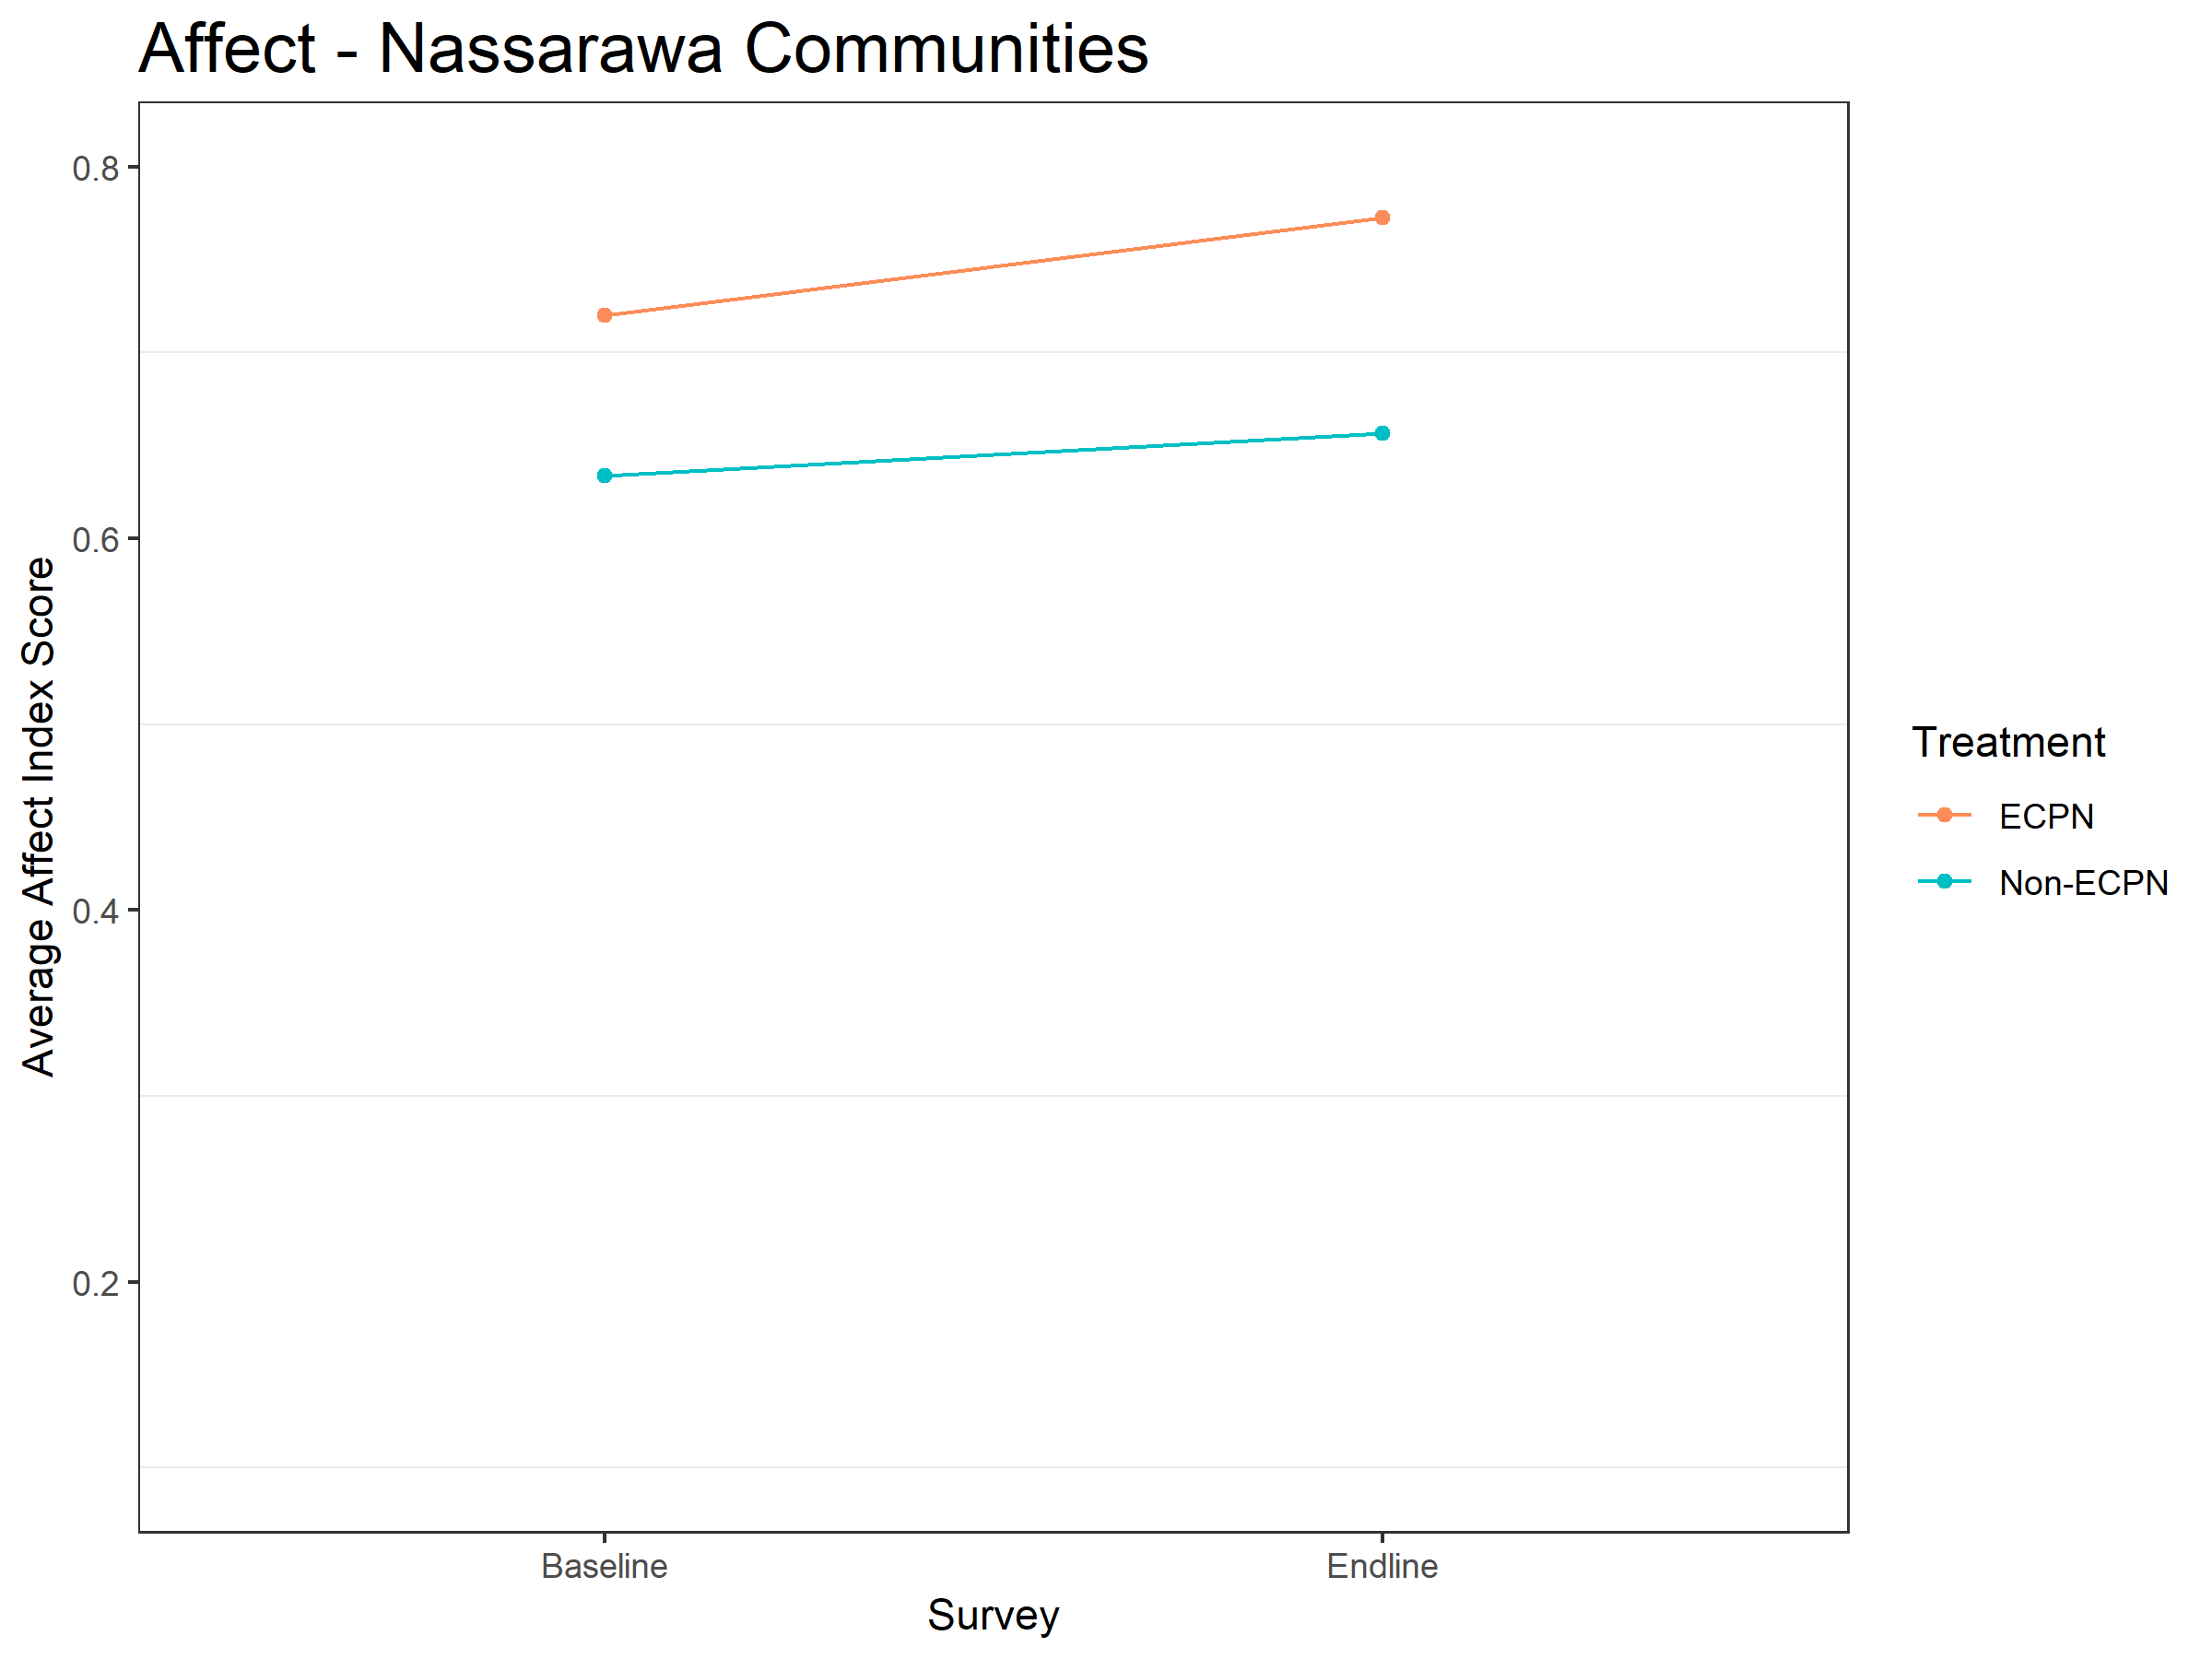
\includegraphics[width=\linewidth]{../../../figs/affectComm_plot_nas.png}
        \caption{\textbf{Descriptive change in community-level intergroup affect from baseline to endline in Nassarawa.} Red line is treatment site average, blue line is control site average.}
        \label{fig:affect_nas}
    \end{subfigure}
    \hfill
    \begin{subfigure}[b]{.48\textwidth}
    \centering
        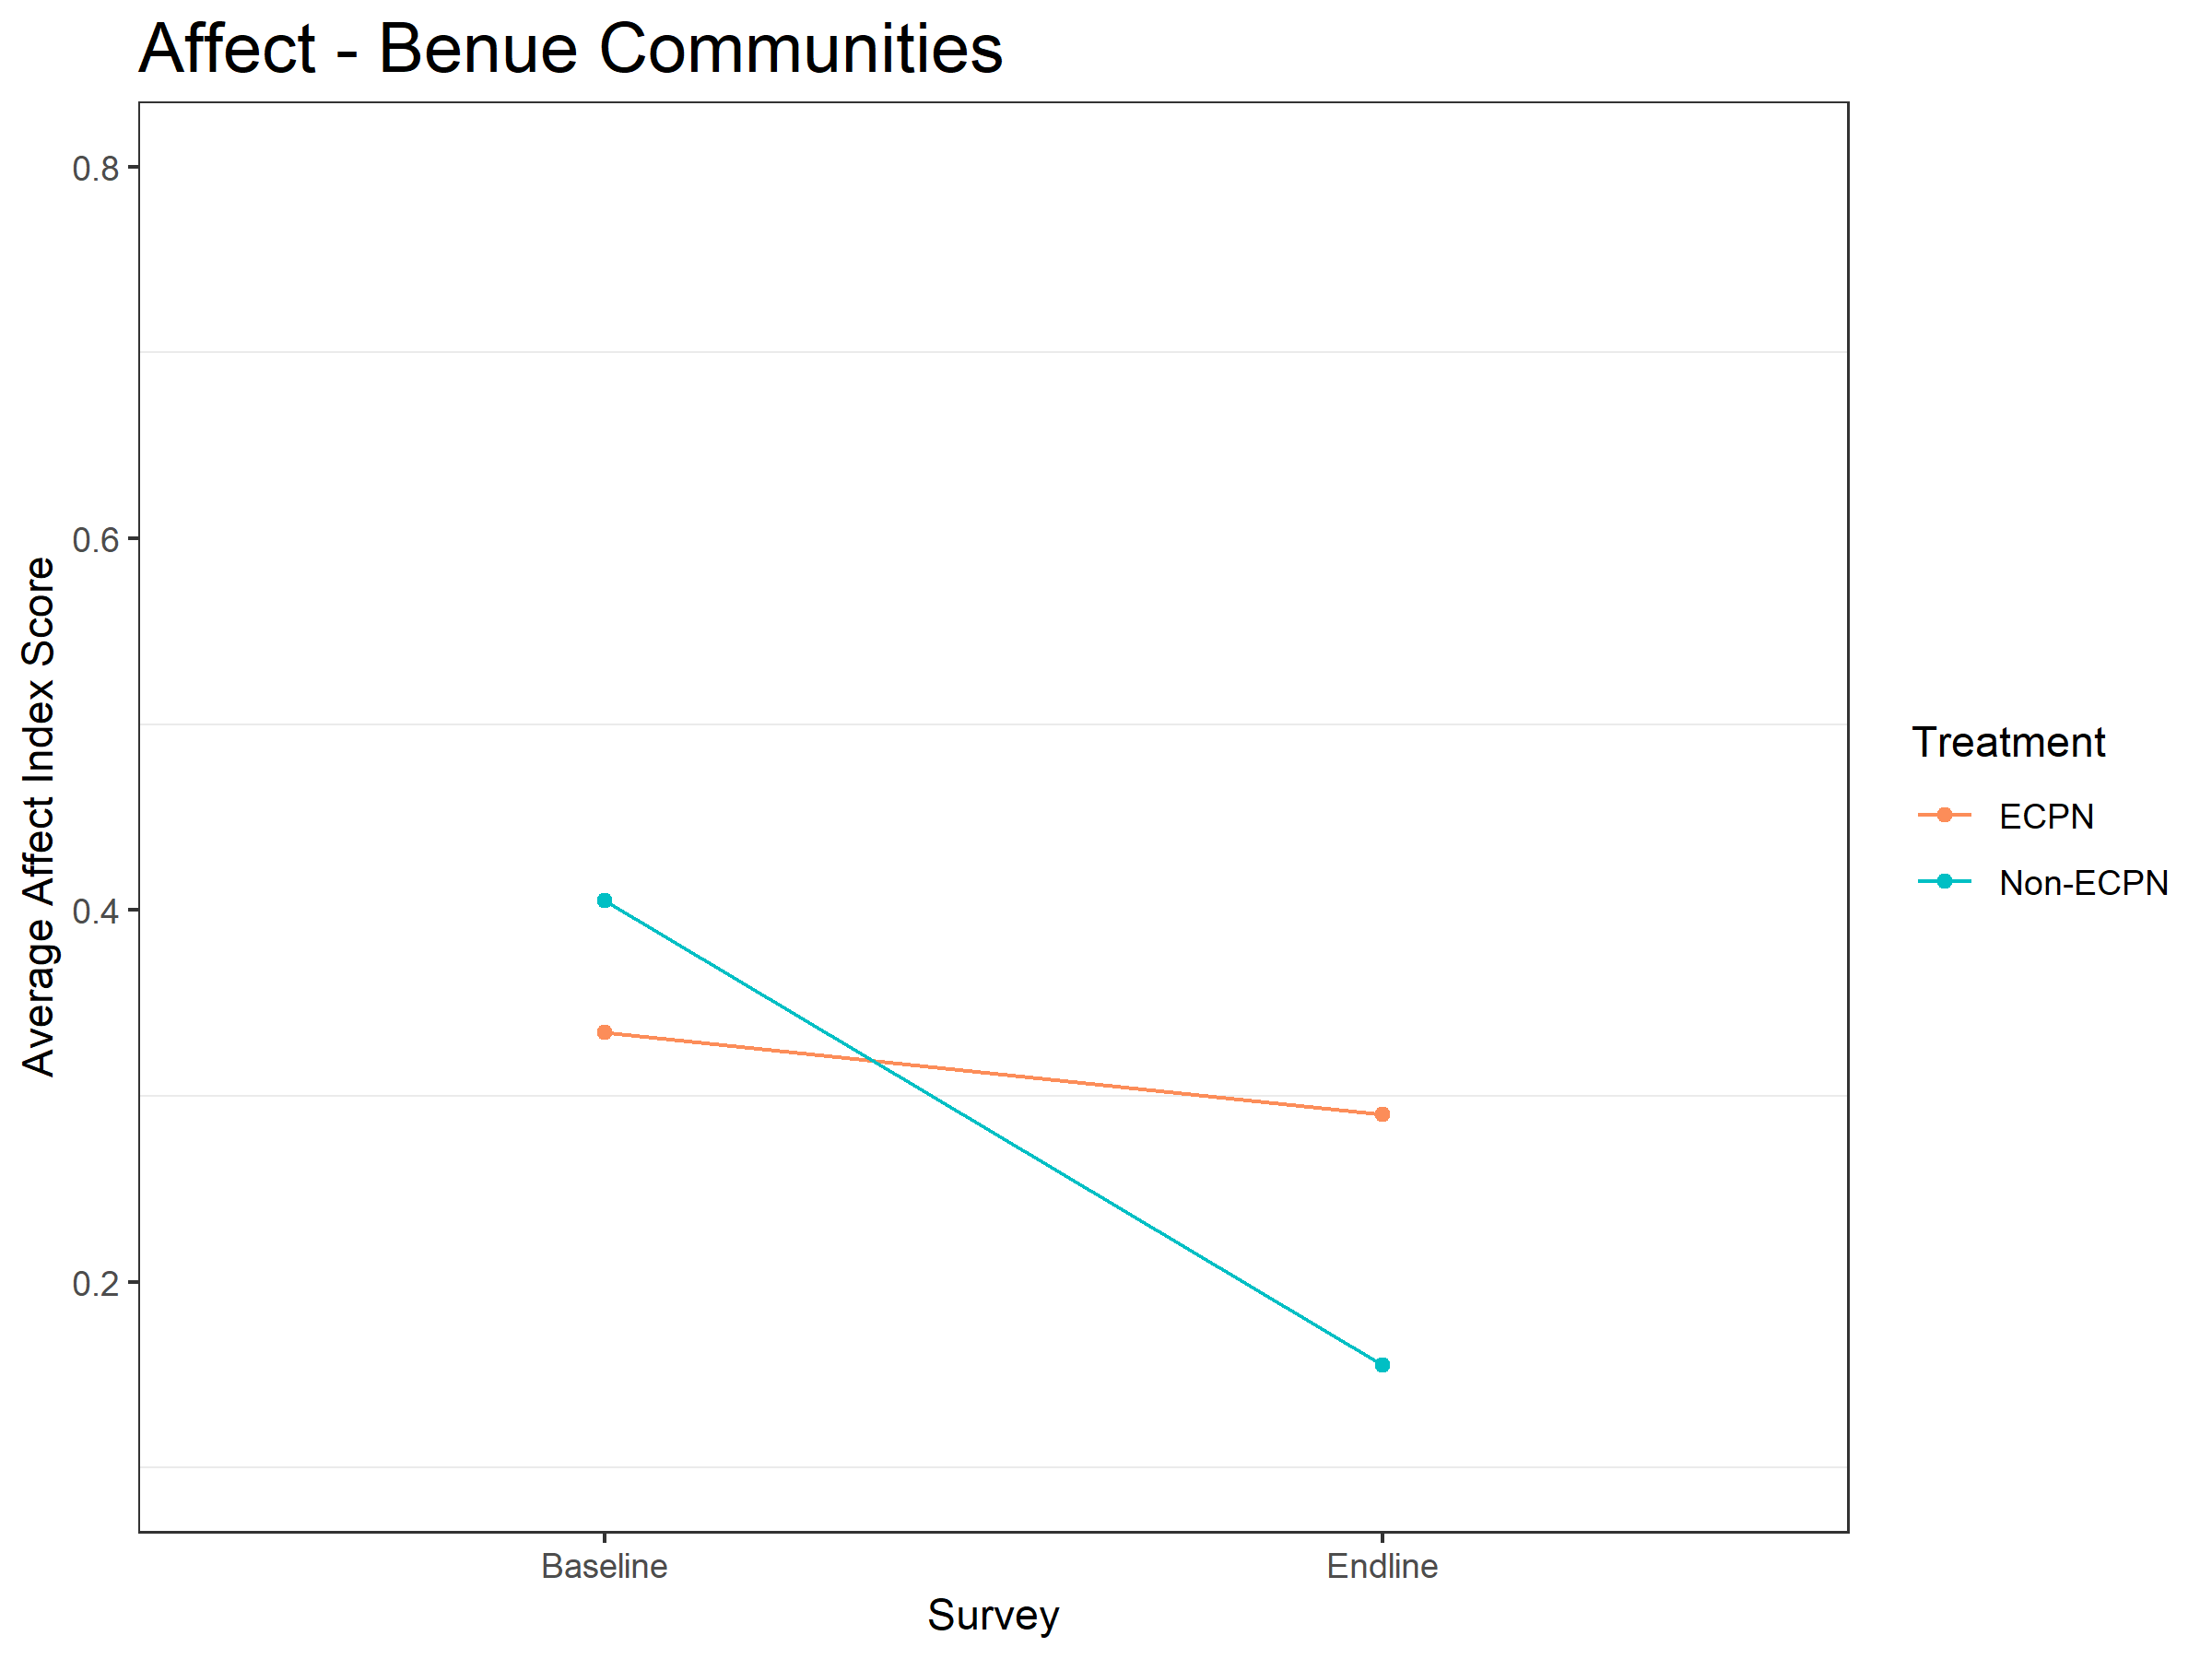
\includegraphics[width=\linewidth]{../../../figs/affectComm_plot_ben.png}
        \caption{\textbf{Descriptive change in community-level intergroup affect from baseline to endline in Benue} Red line is treatment site average, blue line is control site average.}
        \label{fig:affect_ben}
    \end{subfigure}
    \caption{\textbf{State-level intergroup affect.}  Moving up the Y-axis indicates improved affect between groups.}
\end{figure}

\textbf{Contact}: Figure \ref{fig:fig5} above suggested that the
intervention increased contact despite the social environment leading to
a sharp decline in control sites. Figures \ref{fig:con_nas} and
\ref{fig:con_ben} show baseline-endline changes for intergroup contact
in Nassarawa and Benue, respectively. The overall secular decline is
likely due to the displacement in Benue, where intergroup contact went
down for every group, though it declined far less in treatment sites. In
Nassarawa, intergroup contact increased in both treatment and control
sites, but far more in treatment sites. These results suggest that the
intervention increased intergroup contact both in the context of a
pastoralist exodus (Benue), and a pastoralists influx
(Nassarawa).\footnote{These patterns should not be interpreted as floor
  and ceiling effects. Eight of thirty communities reported contact
  higher than the 0.60 mean in Nassarawa, and seven of thirty
  communities reported less contact than the 0.08 mean in Benue. 0.08
  and 0.60 are unlikely to be floor and ceiling when 50\% of communities
  went beyond them.}

\begin{figure}[H]
    \begin{subfigure}[b]{.48\textwidth}
    \centering
        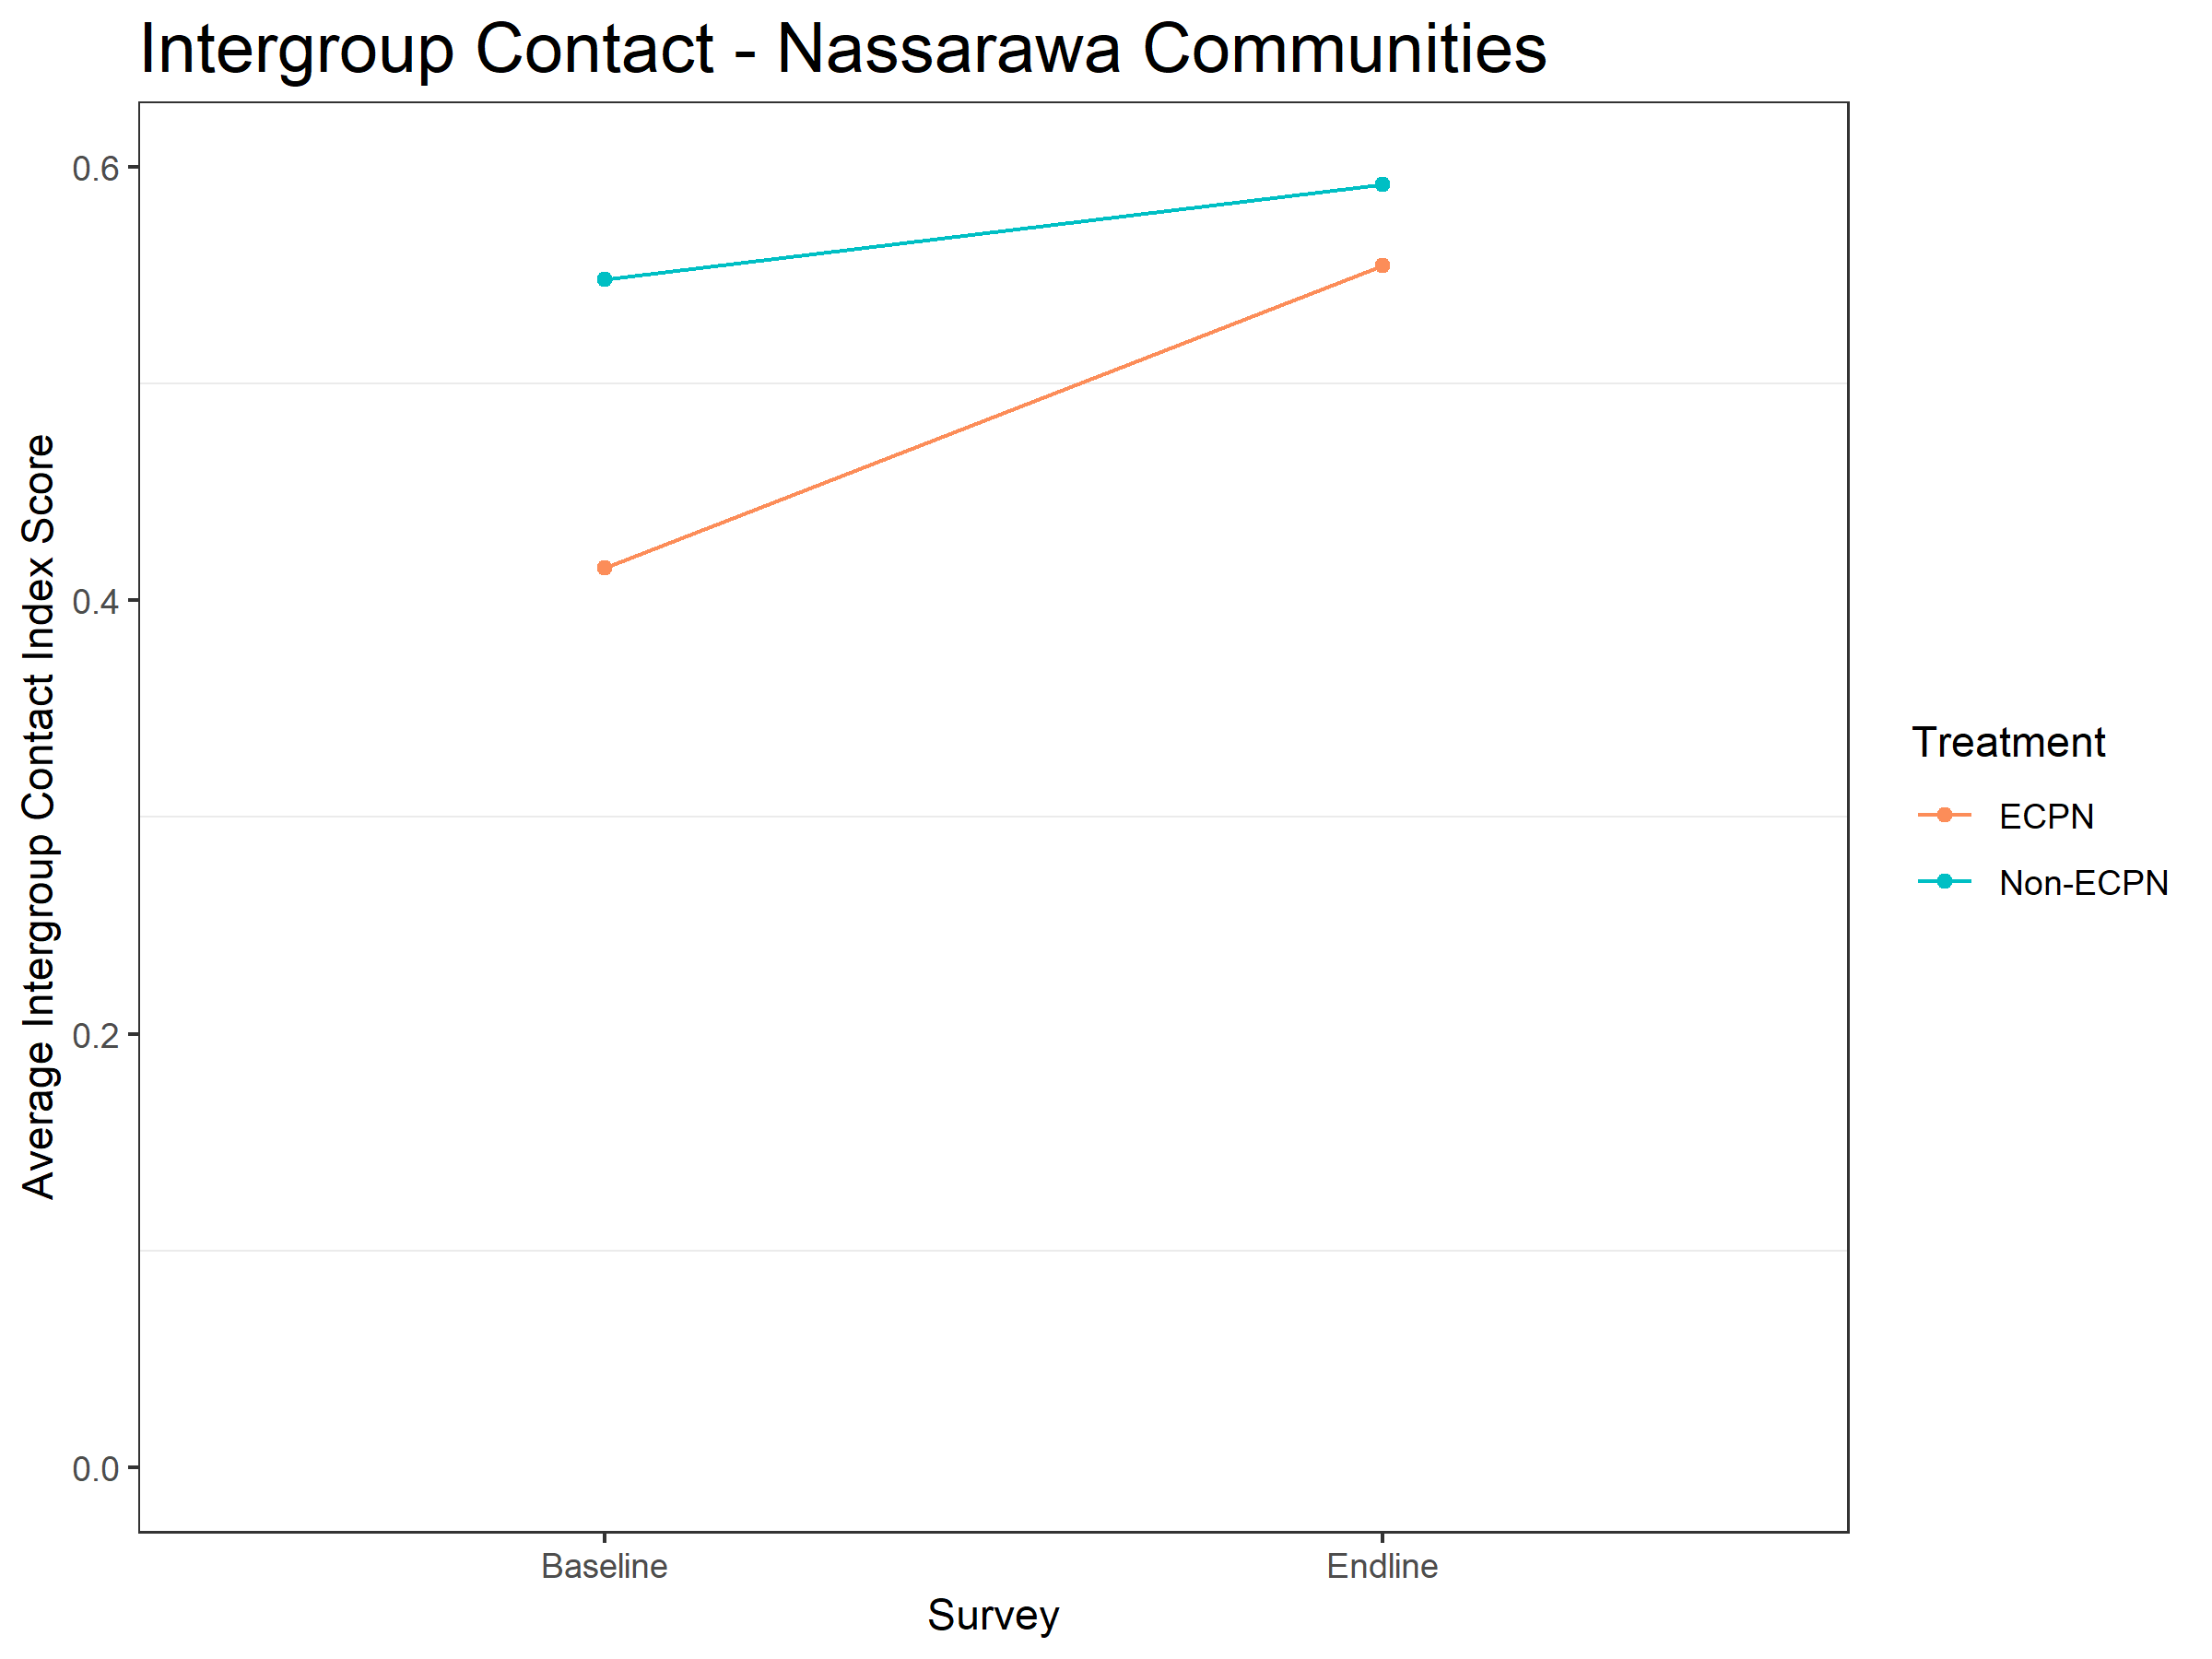
\includegraphics[width=\linewidth]{../../../figs/conComm_plot_nas.png}
        \caption{\textbf{Descriptive change in community-level intergroup contact from baseline to endline in Nassarawa.} Red line is treatment site average, blue line is control site average.}
        \label{fig:con_nas}
    \end{subfigure}
    \hfill
    \begin{subfigure}[b]{.48\textwidth}
    \centering
        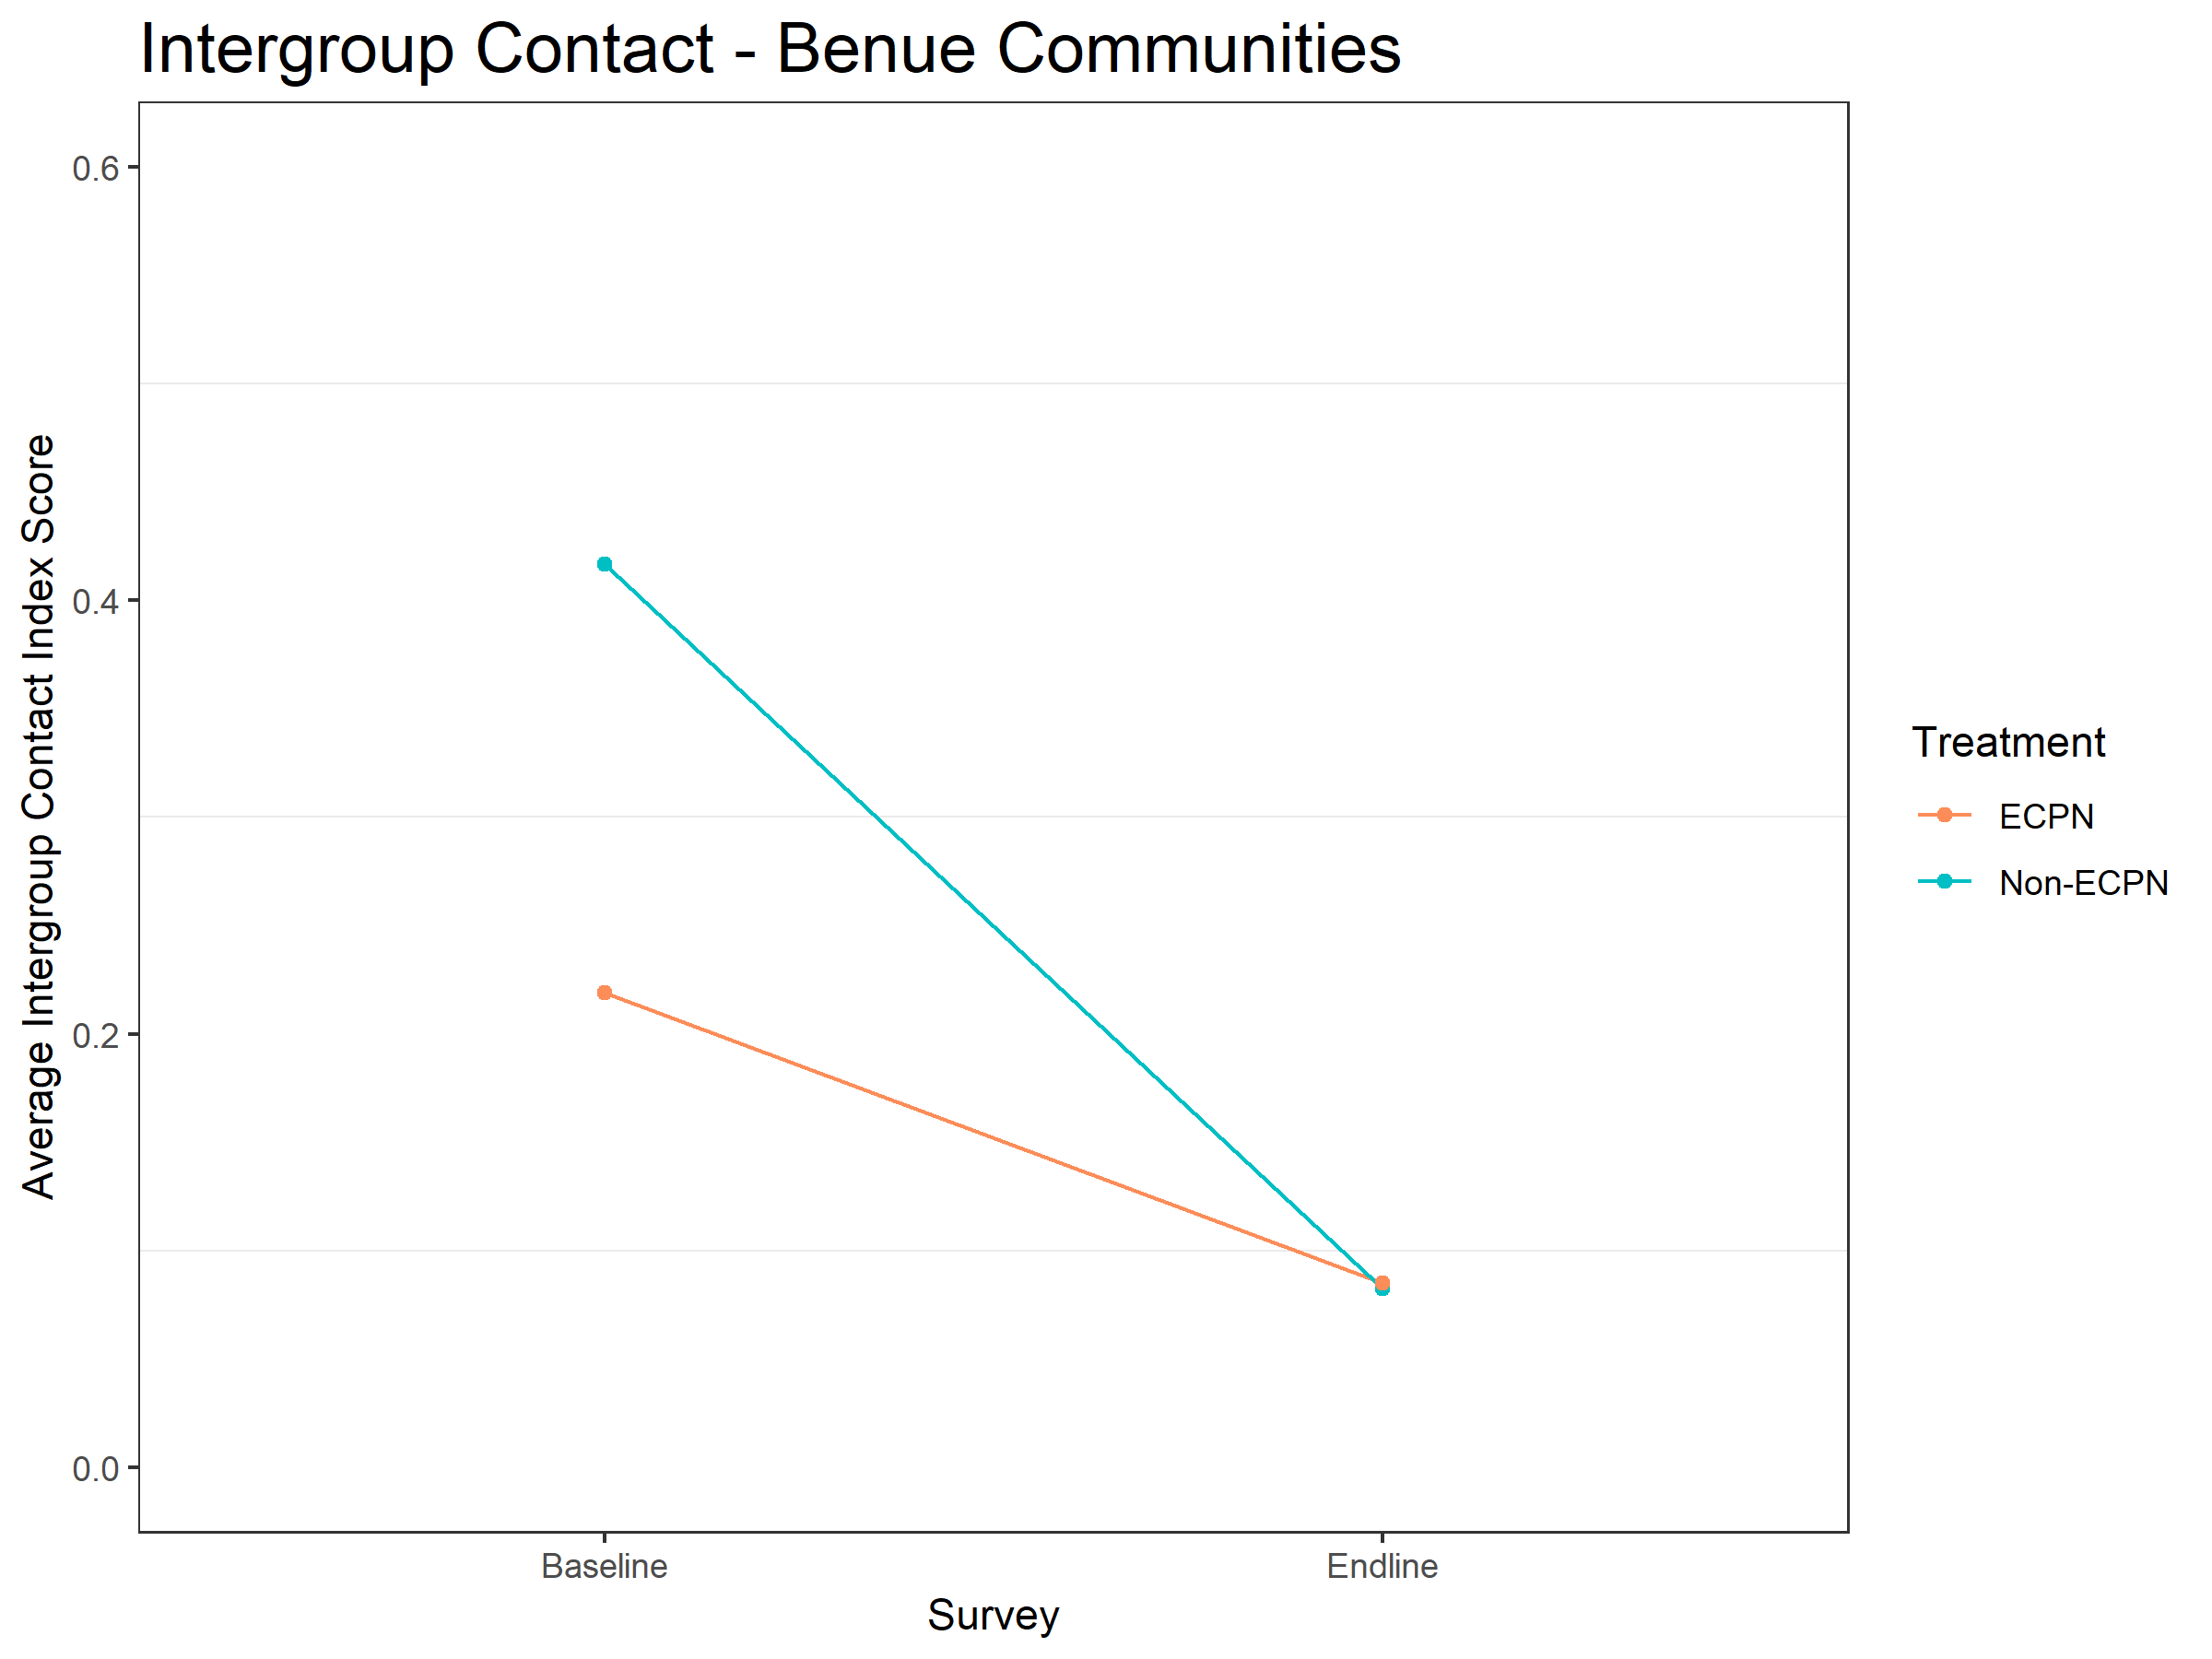
\includegraphics[width=\linewidth]{../../../figs/conComm_plot_ben.png}
        \caption{\textbf{Descriptive change in community-level intergroup contact from baseline to endline in Benue} Red line is treatment site average, blue line is control site average.}
        \label{fig:con_ben}
    \end{subfigure}
    \caption{\textbf{State-level intergroup contact.} Moving up the Y-axis indicates improved contact between groups.}
\end{figure}

\textbf{Perceptions of Physical Security}: The overall analysis above
indicated that perceived physical security improved much more in
intervention sites than in control sites. Figures \ref{fig:in_nas} and
\ref{fig:in_ben} show baseline-endline changes for perceived security in
Nassarawa and Benue, respectively. Perceptions of security in Nassarawa
treatment sites increased substantially, while perceptions of security
in Nassarawa control sites remained unchanged. Perceptions of security
in both treatment and control sites in Benue increased, but moreso in
treatment sites.

\begin{figure}[H]
    \begin{subfigure}[b]{.48\textwidth}
    \centering
        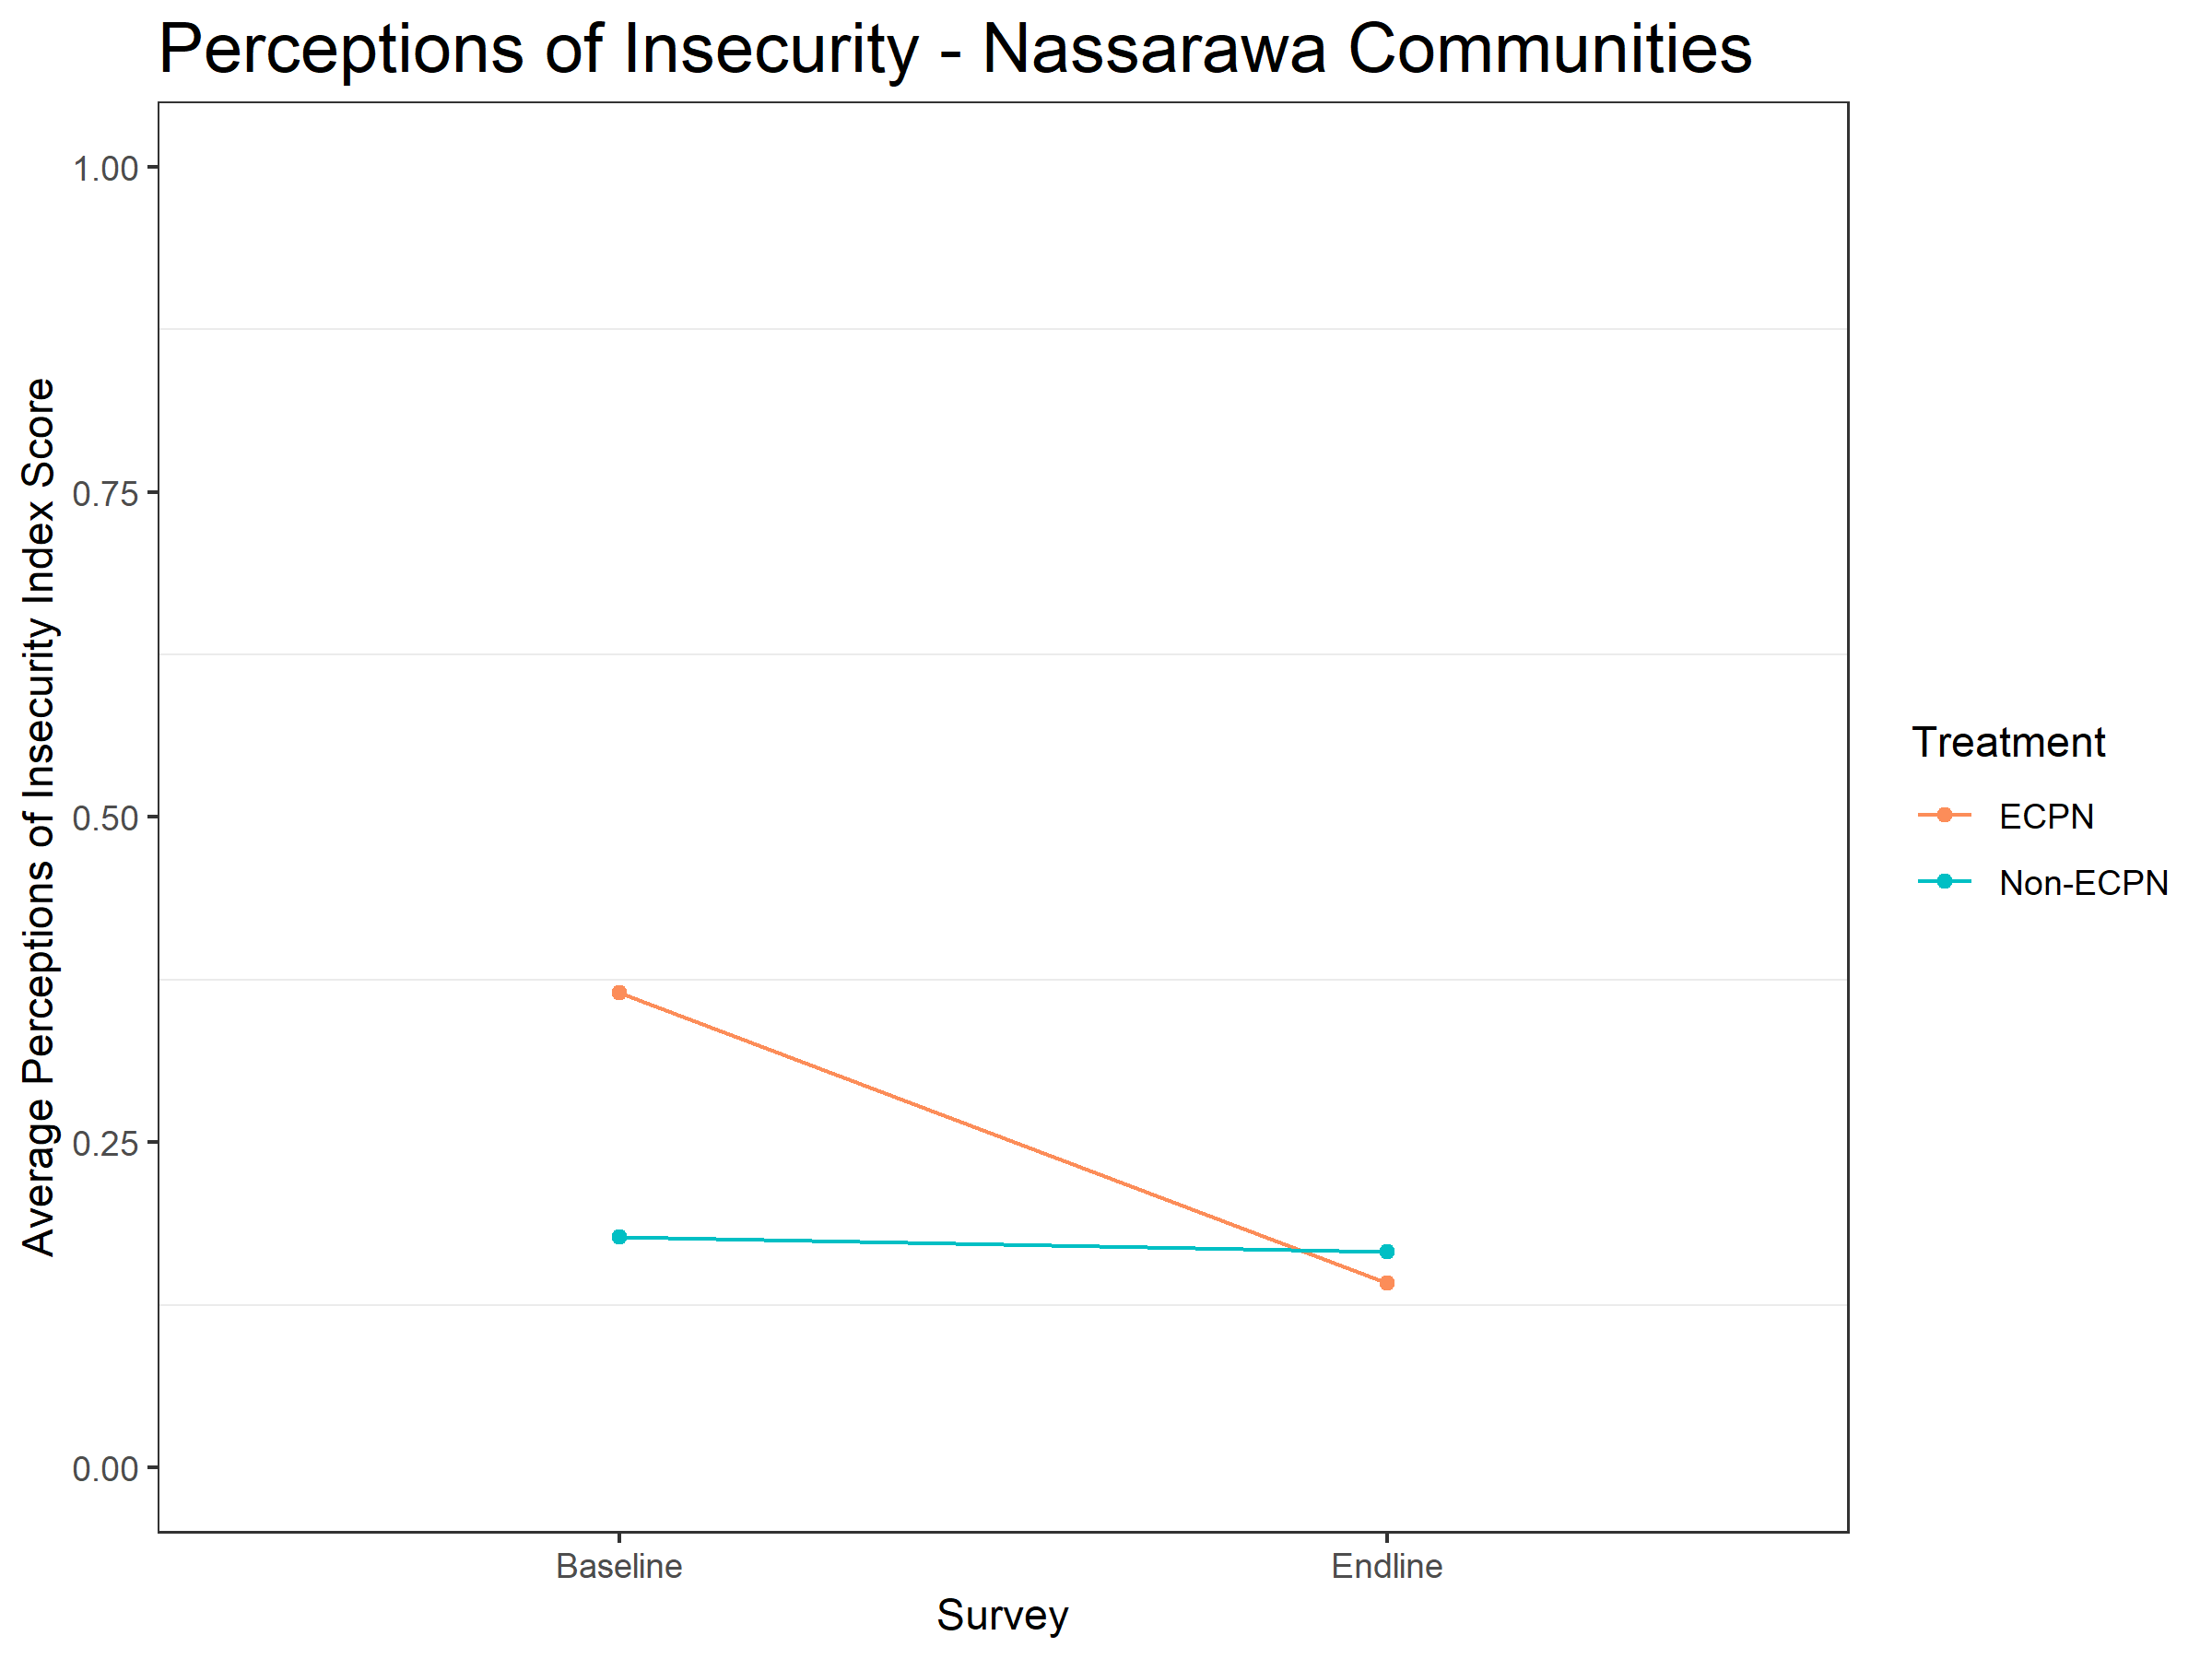
\includegraphics[width=\linewidth]{../../../figs/inComm_plot_nas.png}
        \caption{\textbf{Descriptive change in community-level security from baseline to endline in Nassarawa.} Red line is treatment site average, blue line is control site average.}
        \label{fig:in_nas}
    \end{subfigure}
    \hfill
    \begin{subfigure}[b]{.48\textwidth}
    \centering
        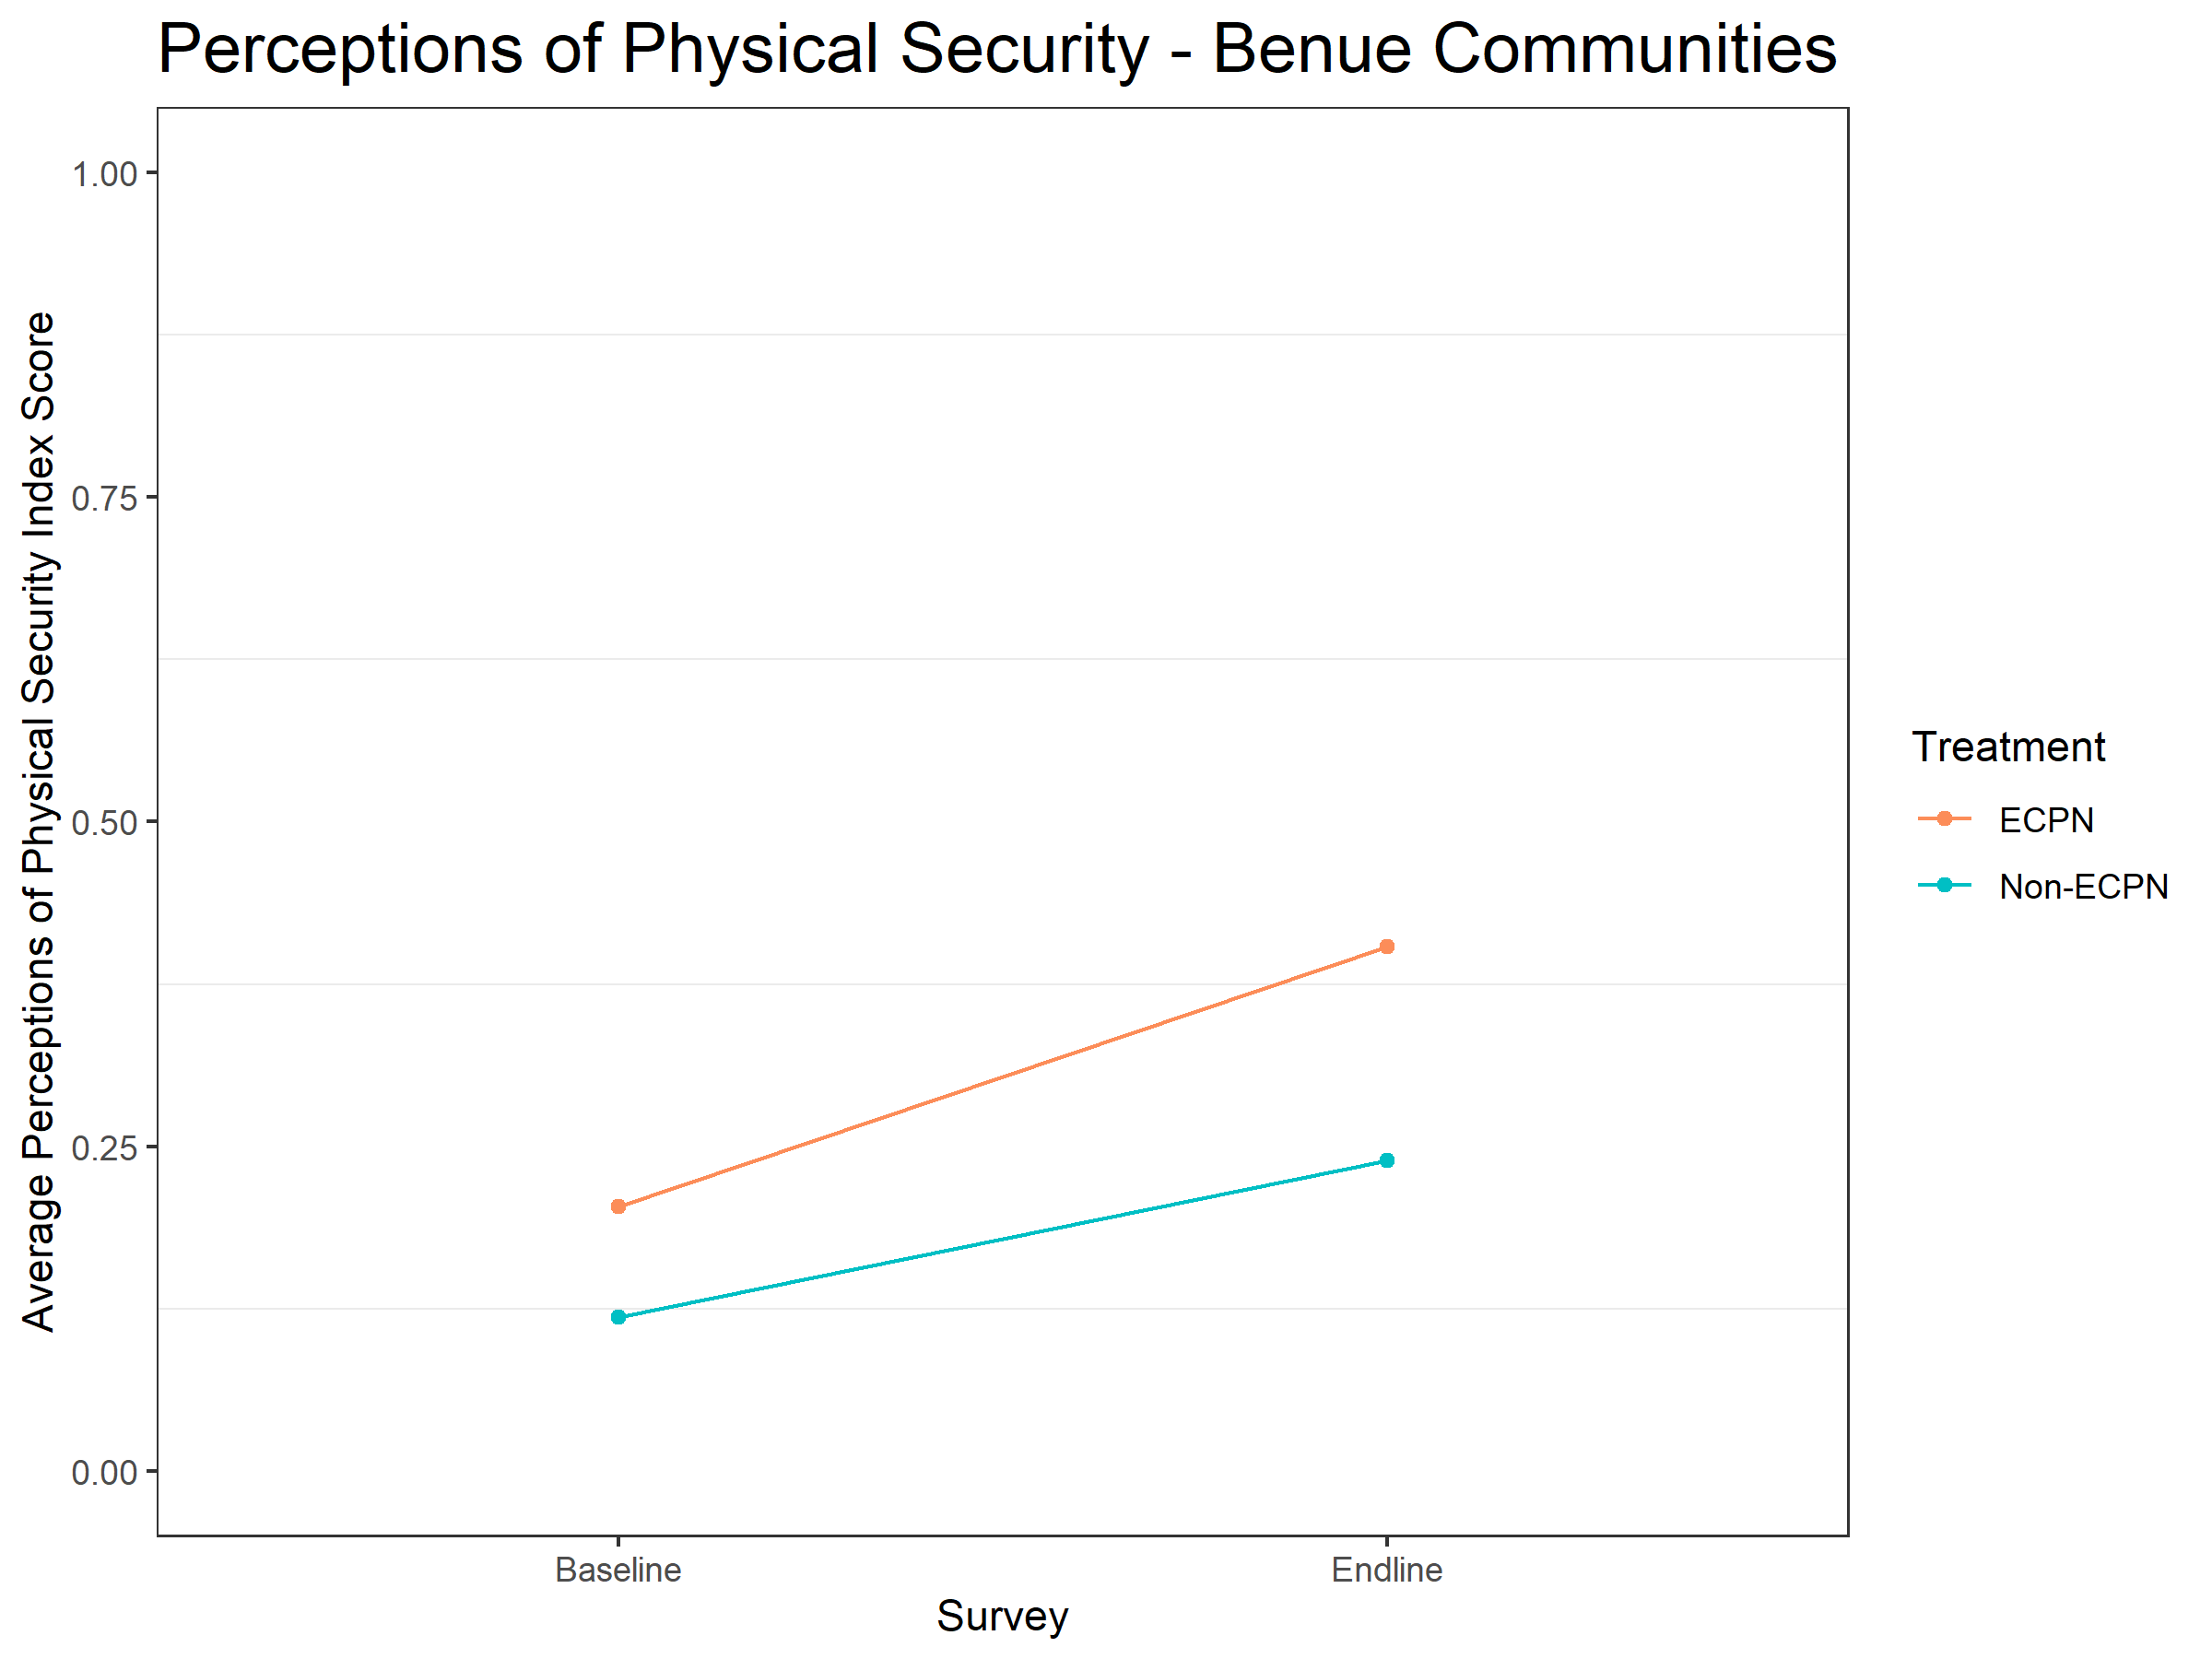
\includegraphics[width=\linewidth]{../../../figs/inComm_plot_ben.png}
        \caption{\textbf{Descriptive change in community-level security from baseline to endline in Benue} Red line is treatment site average, blue line is control site average.}
        \label{fig:in_ben}
    \end{subfigure}
    \caption{\textbf{State-level perceived security.}  Moving up the Y-axis indicates improved security.}
\end{figure}

\hypertarget{social-desirability-bias}{%
\subsection{Social desirability bias}\label{social-desirability-bias}}

To provide evidence that these survey results are due to intergroup
contact and not due to social desirability bias, we analyze the effect
of the intervention on attitudes about violence. Attitudes about
violence are a good candidate for a ``placebo outcome'' because
intergroup contact should not affect general attitudes about violence,
but respondents may feel social pressure to answer violence questions in
a desirable way. If the intervention affects attitudes about violence,
then we worry that other self-reports were affected by social
desirability bias. If the intervention has no effect on attitudes about
violence, then it is unlikely that other self-reports were affected by
social desirability bias. We measure attitudes about violence with a six
question index asking respondents if it is always, sometimes, rarely, or
never justified to use violence in certain situations, such as
retaliating against violence or bringing criminals to justice.

Analysis of this placebo outcome, presented in Appendix C, shows that
the intervention has no effect on attitudes about violence in the
community-level data (\(p\)=0.691) or the individual-level data
(\(p\)=0.556). The coefficients are negative in both cases, so this
result is not due to a lack of statistical power. The lack of an effect
on this placebo outcome, plus our use of survey experiments and
behavioral observation to corroborate survey self-reports, suggests that
our self-report results for primary outcomes are not due to social
desirability bias.

\hypertarget{discussion}{%
\section{Discussion}\label{discussion}}

This paper provides evidence that intergroup contact can improve
intergroup relations, even in dire circumstances. We tested the effects
of a programmatic contact intervention in an active and escalating
conflict between farmers and pastoralists in Nigeria. The persistent
violence of this context and personal involvement of the research
participants poses a stringent test for contact to improve intergroup
relations. The violence generates grievances that feed outgroup
animosity, reinforce group differences, strengthen social and
psychological barriers to improving attitudes, and support the
perception that each groups' interests are opposed. Despite the
difficult context, the program improved intergroup affect, fostered more
intergroup contact, and decreased feelings of insecurity in these
communities.

This study also provides suggestive evidence that the effects of contact
programs, which typically involve only a small subset of a community,
can spillover to others in the community. Respondents from intervention
communities who did not directly participate in our intervention felt
more positive affect toward the other side and felt more physically
secure from violence than control respondents, who were not exposed to
the program at all. These attitudinal and perceptual changes cannot be
explained by increased contact alone. Contact in treatment communities
did increase more than contact in control communities, but contact by
nonparticipants and control respondents increased at the same rate while
affect and perceptions of physical security only increased for
nonparticipants. As a result, we believe that some of the change in
affect and perceptions of security are due to a spillover
effect.\footnote{Another possibility is that no spillover occurred, but
  rather nonparticipants materially benefited from the projects
  completed by the project committees. The project committees improved
  infrastructure useful to the farmer and pastoralist communities, which
  could have reduced resource-based drivers of conflict and influenced
  participants and nonparticipants. This is not spillover, though this
  is another way the intervention could have affected nonparticipants in
  treatment communities.} By examining both direct and indirect
participants, we are able to address a main critique of many
contact-based and peacebuilding interventions: that even if these
interventions change individuals, it is often not clear whether this
change is scalable and will lead to societal change (Ditlmann, Samii,
and Zeitzoff 2017).

We are not able to determine how this spillover from direct to indirect
participants occurred, but we speculate that spillover occurred through
three mechanisms that could shift people's perceptions of how the two
groups can and should interact. First, nonparticipant community members
may have observed members of both groups cooperate to address shared
issues. The intervention established project committees of about 12-15
farmers and pastoralists, and other community members may have learned
from their example. Second, some nonparticipants may have learned about
the other side from personal interactions with participants. Third, and,
we think, most importantly, the intervention may have caused norms of
cooperation and knowledge about the other side to diffuse through each
community. One of the goals of the intervention was to motivate norms
and informal institutions that would impact the entire community and
last beyond the intervention.

Our fieldwork suggests that communities learning about the other side
assisted farmer and pastoralist leaders with mediating intergroup
disputes, such as those caused by cows grazing on farmland. For example,
our research partners on the ground noted that treatment communities
were often able to resolve their disputes because pastoralists became
more aware of the financial value of the crops destroyed by cows and
farmers became more aware of the difficulty of controlling and
corralling thousands of cows; no such learning occurred in control
communities.\footnote{We are especially grateful to Israel Okpe for this
  and other observations about farmer-pastoralist conflict dynamics.}
The intervention could also have encouraged the formation of other
informal institutions that support cooperation, like ingroup policing:
ingroup members punishing other ingroup members who violate the rights
of outgroup members (Ditlmann and Samii 2016; Fearon and Laitin 1996).
As leaders and the project committees established intergroup
cooperation, they may have publicly reprimanded ingroup members who
spoke against the other side or did anything that would hamper the
benefits of cooperation. Visible ingroup policing shows ingroup members
that cooperation is the desirable action and shows outgroup members that
they need not retaliate against the other side.

This paper also contributes to the growing number of field experiments
testing contact theory. One of the major questions emerging from this
literature is whether these interventions shift attitudes, behaviors, or
both. While Scacco and Warren (2018) and Mousa (2020) find changes in
behaviors but not attitudes, Paler et al. (2020) find changes in
attitudes, but not behaviors. One difference between these interventions
is whether the peacebuilding elements of the program were explicit or
implicit. Like Paler et al. (2020), we test an explicit peacebuilding
intervention. We find some changes in attitudes (e.g., outgroup affect)
and some changes in behaviors (e.g., in contact---both self-reported and
observational, but not in the public goods game). Unlike these other
contact-based interventions which ranged from a one-shot meeting (Paler
et al. 2020) to sixteen weeks (Scacco and Warren 2018), ours lasted
eighteen months. That we were able to provide a stronger ``dosage'' of
contact may be one potential explanation why we were able to see changes
in both attitudes and behaviors.

Another difference between these other studies and ours, and perhaps why
we see a spillover effect, is the public nature of the contact. In these
other studies---vocational training, sports and dialogues---the contact
was contained and not broadcasted to the larger community. Our treatment
was much more public, with community leaders holding open fora and the
construction of community infrastructure as a result of joint project
committees. Several recent studies suggest that public information has a
greater impact on attitudes and behaviors than private information
(Adida et al. 2020; Arias 2019; Grossman and Michelitch 2018). In some
cases, maintaining the confidentiality of contact is a necessary
security measure, as was likely the case for Christian and Muslim soccer
players in Mosul (Mousa 2020). In those contexts, those who are willing
to meet with the other side may be considered traitors and targeted by
less tolerant ingroup members. However, by keeping the contact private,
there are fewer opportunities to shift norms of appropriate and accepted
behavior between groups. This could be one reason why we see behaviors
change outside the confines of the intervention -- increased contact in
markets -- while there is little evidence of a change in behaviors off
the sports field in Mosul.\footnote{Although Mousa (2020) found no
  average change in off-field behaviors, the paper found indicative
  evidence that off-field cooperative behaviors improved where the
  soccer leagues were more public and had more community support.}

This study also points to an opportunity for collaboration between
scholars of intergroup contact and scholars of conflict. These
literatures are often concerned with the same end goal --- reducing
conflict --- but rarely speak to one another. Conflict scholars often
see conflict as a bargaining problem, and violence as a bargaining
failure. The conflict literature points to a lack of trust as the
primary cause of conflict and usually posits a strong third party actor
as one effective way of guaranteeing peace. Intergroup contact research
hints that intergroup contact can create cooperative norms and
institutions that serve the same function as a strong third party.
Improving relations -- especially improving trust -- through
psychological interventions like intergroup contact can help groups
overcome trust problems and reduce the likelihood of violence.

There remain several opportunities to learn about the effects of contact
in conflict environments. First, this study employed a design to test
the hypothesis that contact would improve intergroup relations in an
active conflict. Future studies can bring more causal evidence to the
question of how contact improves intergroup relations. For example, does
contact make people more empathetic or able to take the perspective of
the other group? Second, while we see evidence of spillover, we are
unsure how it occurred. Future studies should examine how social norms
and interpersonal discussion diffuse the positive effects of contact to
other ingroup members without outgroup contact. Third, future work
should more deliberately study the dosage of contact necessary to
improve attitudes and behaviors.

Finally, contact interventions, explicitly or implicitly, involve the
groups cooperating to achieve a joint goal. This intervention was
designed to benefit all communities by having the conflicting
communities cooperate successfully. But what if contact is not
successful and the goal is not achieved? Does contact itself still
improve attitudes, or does contact work because groups begin to
associate cross-group cooperation with good outcomes? In a similar vein,
are Allport's conditions necessary for contact to achieve its aims, or
are they only needed insofar as they ensure the intergroup cooperation
generates positive outcomes for both groups? Future studies should
determine the necessity of Allport's conditions and attempt to
differentiate the fact of contact from the outcomes that group
cooperation produces.

\hypertarget{references}{%
\section*{References}\label{references}}
\addcontentsline{toc}{section}{References}

\hypertarget{refs}{}
\begin{cslreferences}
\leavevmode\hypertarget{ref-adida2020does}{}%
Adida, Claire, Jessica Gottlieb, Eric Kramon, and Gwyneth McClendon.
2020. ``When Does Information Influence Voters? The Joint Importance of
Salience and Coordination.'' \emph{Comparative Political Studies} 53(6):
851--91.

\leavevmode\hypertarget{ref-nyt2018nigeria}{}%
Akinwotu, Emmanuel. 2018. ``Nigeria's Farmers and Herders Fight a Deadly
Battle for Scarce Resources.'' \emph{New York Times}.
\url{https://www.nytimes.com/2018/06/25/world/africa/nigeria-herders-farmers.html}.

\leavevmode\hypertarget{ref-allport1954prejudice}{}%
Allport, Gordon. 1954. ``The Nature of Prejudice.'' \emph{Garden City,
NJ Anchor}.

\leavevmode\hypertarget{ref-arias2019does}{}%
Arias, Eric. 2019. ``How Does Media Influence Social Norms? Experimental
Evidence on the Role of Common Knowledge.'' \emph{Political Science
Research and Methods} 7(3): 561--78.

\leavevmode\hypertarget{ref-barlow2012contact}{}%
Barlow, Fiona Kate et al. 2012. ``The Contact Caveat: Negative Contact
Predicts Increased Prejudice More Than Positive Contact Predicts Reduced
Prejudice.'' \emph{Personality and Social Psychology Bulletin} 38(12):
1629--43.

\leavevmode\hypertarget{ref-bar2000intractable}{}%
Bar-Tal, Daniel. 2000. ``From Intractable Conflict Through Conflict
Resolution to Reconciliation: Psychological Analysis.'' \emph{Political
Psychology} 21(2): 351--65.

\leavevmode\hypertarget{ref-bar2007sociopsychological}{}%
---------. 2007. ``Sociopsychological Foundations of Intractable
Conflicts.'' \emph{American Behavioral Scientist} 50(11): 1430--53.

\leavevmode\hypertarget{ref-bar2017development}{}%
Bar-Tal, Daniel, and Talia Avrahamzon. 2017. ``Development of
Delegitimization and Animosity in the Context of Intractable Conflict.''

\leavevmode\hypertarget{ref-bassett2009mobile}{}%
Bassett, Thomas J. 2009. ``Mobile Pastoralism on the Brink of Land
Privatization in Northern côte d'Ivoire.'' \emph{Geoforum} 40(5):
756--66.

\leavevmode\hypertarget{ref-batson1997empathy}{}%
Batson, C Daniel et al. 1997. ``Empathy and Attitudes: Can Feeling for a
Member of a Stigmatized Group Improve Feelings Toward the Group?''
\emph{Journal of personality and social psychology} 72(1): 105.

\leavevmode\hypertarget{ref-boisjoly2006empathy}{}%
Boisjoly, Johanne et al. 2006. ``Empathy or Antipathy? The Impact of
Diversity.'' \emph{American Economic Review} 96(5): 1890--1905.

\leavevmode\hypertarget{ref-bornstein2003intergroup}{}%
Bornstein, Gary. 2003. ``Intergroup Conflict: Individual, Group, and
Collective Interests.'' \emph{Personality and social psychology review}
7(2): 129--45.

\leavevmode\hypertarget{ref-broockman2016durably}{}%
Broockman, David, and Joshua Kalla. 2016. ``Durably Reducing
Transphobia: A Field Experiment on Door-to-Door Canvassing.''
\emph{Science} 352(6282): 220--24.

\leavevmode\hypertarget{ref-burns2015interaction}{}%
Burns, Justine, Lucia Corno, and Eliana La Ferrara. 2015.
\emph{Interaction, Prejudice and Performance. Evidence from South
Africa}. Working paper.

\leavevmode\hypertarget{ref-carrell2015impact}{}%
Carrell, Scott E, Mark Hoekstra, and James E West. 2015. \emph{The
Impact of Intergroup Contact on Racial Attitudes and Revealed
Preferences}. National Bureau of Economic Research.

\leavevmode\hypertarget{ref-chang2019building}{}%
Chang, Han Il, and Leonid Peisakhin. 2019. ``Building Cooperation Among
Groups in Conflict: An Experiment on Intersectarian Cooperation in
Lebanon.'' \emph{American Journal of Political Science} 63(1): 146--62.

\leavevmode\hypertarget{ref-christ2014contextual}{}%
Christ, Oliver et al. 2014. ``Contextual Effect of Positive Intergroup
Contact on Outgroup Prejudice.'' \emph{Proceedings of the National
Academy of Sciences} 111(11): 3996--4000.

\leavevmode\hypertarget{ref-cook1985experimenting}{}%
Cook, Stuart W. 1985. ``Experimenting on Social Issues: The Case of
School Desegregation.'' \emph{American Psychologist} 40(4): 452.

\leavevmode\hypertarget{ref-cook1971race}{}%
Cook, Stuart Wellford, Lawrence Samuel Wrightsman, and Shirley
Wrightsman. 1971. \emph{The Effect of Unintended Interracial Contact
Upon Racial Interaction and Attitude Change}. Educational resources in
information center, US Department of health, education \& welfare.

\leavevmode\hypertarget{ref-cotula2004land}{}%
Cotula, Lorenzo, Camilla Toulmin, Ced Hesse, and others. 2004.
\emph{Land Tenure and Administration in Africa: Lessons of Experience
and Emerging Issues}. International Institute for Environment;
Development London.

\leavevmode\hypertarget{ref-daniel2018anti}{}%
Daniel, Soni. 2018. ``Anti-Open Grazing Law: Nass, Benue, Kwara, Taraba
Tackle Defence Minister.'' \emph{Vanguard}.
\url{https://www.vanguardngr.com/2018/06/anti-open-grazing-law-nass-benue-kwara-taraba-tackle-defence-minister/}.

\leavevmode\hypertarget{ref-deutsch1973resolution}{}%
Deutsch, Morton. 1973. \emph{The Resolution of Conflict: Constructive
and Destructive Processes}. Yale University Press.

\leavevmode\hypertarget{ref-deutsch1951interracial}{}%
Deutsch, Morton, and Mary Evans Collins. 1951. \emph{Interracial
Housing: A Psychological Evaluation of a Social Experiment}. U of
Minnesota Press.

\leavevmode\hypertarget{ref-ditlmann2016can}{}%
Ditlmann, Ruth K, and Cyrus Samii. 2016. ``Can Intergroup Contact Affect
Ingroup Dynamics? Insights from a Field Study with Jewish and
Arab-Palestinian Youth in Israel.'' \emph{Peace and Conflict: Journal of
Peace Psychology} 22(4): 380.

\leavevmode\hypertarget{ref-ditlmann2017addressing}{}%
Ditlmann, Ruth K, Cyrus Samii, and Thomas Zeitzoff. 2017. ``Addressing
Violent Intergroup Conflict from the Bottom up?'' \emph{Social Issues
and Policy Review} 11(1): 38--77.

\leavevmode\hypertarget{ref-doosje1995bad}{}%
Doosje, Bertjan, Russell Spears, and Willem Koomen. 1995. ``When Bad
Isn't All Bad: Strategic Use of Sample Information in Generalization and
Stereotyping.'' \emph{Journal of Personality and Social psychology}
69(4): 642.

\leavevmode\hypertarget{ref-duru2018court}{}%
Duru, Peter. 2018. ``Court Stops Inspector General from Proscribing
Benue Livestock Guard.'' \emph{Vanguard}.
\url{https://www.vanguardngr.com/2018/11/court-stops-ig-from-proscribing-benue-livestock-guards/}.

\leavevmode\hypertarget{ref-enos2014causal}{}%
Enos, Ryan D. 2014. ``Causal Effect of Intergroup Contact on
Exclusionary Attitudes.'' \emph{Proceedings of the National Academy of
Sciences} 111(10): 3699--3704.

\leavevmode\hypertarget{ref-fearon1995rationalist}{}%
Fearon, James D. 1995. ``Rationalist Explanations for War.''
\emph{International organization} 49(3): 379--414.

\leavevmode\hypertarget{ref-fearon2009can}{}%
Fearon, James D, Macartan Humphreys, and Jeremy M Weinstein. 2009. ``Can
Development Aid Contribute to Social Cohesion After Civil War? Evidence
from a Field Experiment in Post-Conflict Liberia.'' \emph{The American
Economic Review} 99(2): 287--91.

\leavevmode\hypertarget{ref-fearon1996explaining}{}%
Fearon, James D, and David D Laitin. 1996. ``Explaining Interethnic
Cooperation.'' \emph{American political science review} 90(4): 715--35.

\leavevmode\hypertarget{ref-fearon2000violence}{}%
---------. 2000. ``Violence and the Social Construction of Ethnic
Identity.'' \emph{International organization} 54(4): 845--77.

\leavevmode\hypertarget{ref-festinger1962cognitiveDissonance}{}%
Festinger, Leon. 1962. 2 \emph{A Theory of Cognitive Dissonance}.
Stanford university press.

\leavevmode\hypertarget{ref-finseraas2016women}{}%
Finseraas, Henning, Åshild A Johnsen, Andreas Kotsadam, and Gaute
Torsvik. 2016. ``Exposure to Female Colleagues Breaks the Glass
Ceiling---Evidence from a Combined Vignette and Field Experiment.''
\emph{European Economic Review} 90: 363--74.

\leavevmode\hypertarget{ref-gaertner2014reducing}{}%
Gaertner, Samuel L, and John F Dovidio. 2014. \emph{Reducing Intergroup
Bias: The Common Ingroup Identity Model}. Psychology Press.

\leavevmode\hypertarget{ref-gaertner1993common}{}%
Gaertner, Samuel L et al. 1993. ``The Common Ingroup Identity Model:
Recategorization and the Reduction of Intergroup Bias.'' \emph{European
review of social psychology} 4(1): 1--26.

\leavevmode\hypertarget{ref-grossman2018information}{}%
Grossman, Guy, and Kristin Michelitch. 2018. ``Information
Dissemination, Competitive Pressure, and Politician Performance Between
Elections: A Field Experiment in Uganda.'' \emph{The American Political
Science Review} 112(2): 280--301.

\leavevmode\hypertarget{ref-gubler2013humanizing}{}%
Gubler, Joshua R. 2013. ``When Humanizing the Enemy Fails: The Role of
Dissonance and Justification in Intergroup Conflict.'' In \emph{Annual
Meeting of the American Political Science Association},

\leavevmode\hypertarget{ref-frontera2018nigeria}{}%
Hailemariam, Adium. 2018. ``Nigeria: Violence in the Middle Belt Becomes
Major Concern for President Buhari.'' \emph{Frontera}.
\url{https://frontera.net/news/africa/nigeria-violence-in-the-middle-belt-becomes-major-concern-for-president-buhari/}.

\leavevmode\hypertarget{ref-harrison2004field}{}%
Harrison, Glenn W, and John A List. 2004. ``Field Experiments.''
\emph{Journal of Economic literature} 42(4): 1009--55.

\leavevmode\hypertarget{ref-council2019nigeria}{}%
Harwood, Asch. 2019. ``Update: The Numbers Behind Sectarian Violence in
Nigeria.'' \emph{Council on Foreign Relations}.
\url{https://www.cfr.org/blog/update-numbers-behind-sectarian-violence-nigeria}.

\leavevmode\hypertarget{ref-fa2019deadly}{}%
Ilo, Udo Jude, Jonathan-Ichavar Ier, and Yemi Adamolekun. 2019. ``The
Deadliest Conflict You've Never Heard of: Nigeria's Cattle Herders and
Farmers Wage a Resource War.'' \emph{Foreign Affairs}.
\url{https://www.foreignaffairs.com/articles/nigeria/2019-01-23/deadliest-conflict-youve-never-heard}.

\leavevmode\hypertarget{ref-kazeem2018ag}{}%
Kazeem, Yomi. 2018. ``Nigeria's Deadly Pastoral Attacks Are Hurting the
Potential of an Agric-Powered Economy.'' \emph{Quartz Africa}.

\leavevmode\hypertarget{ref-kertzer2018empathy}{}%
Kertzer, Joshua D, Ryan Brutger, and Kai Quek. 2018. ``Strategic Empathy
and the Security Dilemma: Cross-National Experimental Evidence from
China and the United States.''

\leavevmode\hypertarget{ref-klein1992motivated}{}%
Klein, William M, and Ziva Kunda. 1992. ``Motivated Person Perception:
Constructing Justifications for Desired Beliefs.'' \emph{Journal of
experimental social psychology} 28(2): 145--68.

\leavevmode\hypertarget{ref-kunda1990motivatedReasoning}{}%
Kunda, Ziva. 1990. ``The Case for Motivated Reasoning.''
\emph{Psychological bulletin} 108(3): 480.

\leavevmode\hypertarget{ref-kuusaana2015land}{}%
Kuusaana, Elias Danyi, and Kaderi Noagah Bukari. 2015. ``Land Conflicts
Between Smallholders and Fulani Pastoralists in Ghana: Evidence from the
Asante Akim North District (Aand).'' \emph{Journal of rural studies} 42:
52--62.

\leavevmode\hypertarget{ref-lemmer2015can}{}%
Lemmer, Gunnar, and Ulrich Wagner. 2015. ``Can We Really Reduce Ethnic
Prejudice Outside the Lab? A Meta-Analysis of Direct and Indirect
Contact Interventions.'' \emph{European Journal of Social Psychology}
45(2): 152--68.

\leavevmode\hypertarget{ref-lowe2020types}{}%
Lowe, Matt. 2020. ``Types of Contact: A Field Experiment on
Collaborative and Adversarial Caste Integration.''

\leavevmode\hypertarget{ref-marmaros2006friendships}{}%
Marmaros, David, and Bruce Sacerdote. 2006. ``How Do Friendships Form?''
\emph{The Quarterly Journal of Economics} 121(1): 79--119.

\leavevmode\hypertarget{ref-mcdonnel2017graze}{}%
McDonnel, Tim. 2017. ``Why It's Now a Crime to Let Cattle Graze Freely
in 2 Nigerian States.'' \emph{National Public Radio (NPR)}.
\url{https://www.npr.org/sections/goatsandsoda/2017/12/12/569913821/why-its-now-a-crime-to-let-cattle-graze-freely-in-2-nigerian-states}.

\leavevmode\hypertarget{ref-mcdougal2015effect}{}%
McDougal, Topher L et al. 2015. ``The Effect of Farmer-Pastoralist
Violence on Income: New Survey Evidence from Nigeria's Middle Belt
States.'' \emph{Economics of Peace and Security Journal} 10(1): 54--65.

\leavevmode\hypertarget{ref-mousa2020building}{}%
Mousa, Salma. 2020. ``Building Social Cohesion Between Christians and
Muslims Through Soccer in Post-Isis Iraq.'' \emph{Science} 369(6505):
866--70.

\leavevmode\hypertarget{ref-nigeria2014freedom}{}%
Network, Nigeria Research. 2014. ``Indigeneity, Belonging, and Religious
Freedom in Nigeria: Citizens' Views from the Street.'' \emph{5. NRN
Policy Brief}.
\url{https://www.researchgate.net/publication/333320680_Indigeneity_Belonging_Religious_Freedom_in_Nigeria}.

\leavevmode\hypertarget{ref-nickerson1998confirmation}{}%
Nickerson, Raymond S. 1998. ``Confirmation Bias: A Ubiquitous Phenomenon
in Many Guises.'' \emph{Review of general psychology} 2(2): 175--220.

\leavevmode\hypertarget{ref-hrw2018farmer}{}%
Nnoko-Mewanu, Juliana. 2018. ``Farmer-Herder Conflict on the Rise in
Africa.'' \emph{Human Rights Watch}.

\leavevmode\hypertarget{ref-okpara2015conflicts}{}%
Okpara, Uche T, Lindsay C Stringer, Andrew J Dougill, and Mohammed D
Bila. 2015. ``Conflicts About Water in Lake Chad: Are Environmental,
Vulnerability and Security Issues Linked?'' \emph{Progress in
Development Studies} 15(4): 308--25.

\leavevmode\hypertarget{ref-page2008little}{}%
Page-Gould, Elizabeth, Rodolfo Mendoza-Denton, and Linda R Tropp. 2008.
``With a Little Help from My Cross-Group Friend: Reducing Anxiety in
Intergroup Contexts Through Cross-Group Friendship.'' \emph{Journal of
personality and social psychology} 95(5): 1080.

\leavevmode\hypertarget{ref-paler2020cross}{}%
Paler, Laura, Leslie Marshall, Sami Atallah, and others. 2020. ``How
Cross-Cutting Discussion Shapes Support for Ethnic Politics: Evidence
from an Experiment in Lebanon.'' \emph{Quarterly Journal of Political
Science} 15(1): 33--71.

\leavevmode\hypertarget{ref-paluck2009jsp}{}%
Paluck, Elizabeth Levy. 2009. ``Reducing Intergroup Prejudice and
Conflict Using the Media: A Field Experiment in Rwanda.'' \emph{Journal
of personality and social psychology} 96(3): 574.

\leavevmode\hypertarget{ref-paluck2019contact}{}%
Paluck, Elizabeth Levy, Seth A Green, and Donald P Green. 2019. ``The
Contact Hypothesis Re-Evaluated.'' \emph{Behavioural Public Policy}
3(2): 129--58.

\leavevmode\hypertarget{ref-paolini2010negative}{}%
Paolini, Stefania, Jake Harwood, and Mark Rubin. 2010. ``Negative
Intergroup Contact Makes Group Memberships Salient: Explaining Why
Intergroup Conflict Endures.'' \emph{Personality and Social Psychology
Bulletin} 36(12): 1723--38.

\leavevmode\hypertarget{ref-pettigrew2006meta}{}%
Pettigrew, Thomas F, and Linda R Tropp. 2006. ``A Meta-Analytic Test of
Intergroup Contact Theory.'' \emph{Journal of personality and social
psychology} 90(5): 751.

\leavevmode\hypertarget{ref-rao2019familiarity}{}%
Rao, Gautam. 2019. ``Familiarity Does Not Breed Contempt: Generosity,
Discrimination, and Diversity in Delhi Schools.'' \emph{American
Economic Review} 109(3): 774--809.

\leavevmode\hypertarget{ref-rigterink2019isa}{}%
Rigterink, Anouk, and Mareike Schomerus. 2019. ``Behavioural
Experiments, Micro-Narratives, Structured Survey and Interviews:
Combining Four Methods to Understand How Past Violent Conflict Affects
Behaviour.''

\leavevmode\hypertarget{ref-rime2011impact}{}%
Rimé, Bernard, Patrick Kanyangara, Vincent Yzerbyt, and Dario Paez.
2011. ``The Impact of Gacaca Tribunals in Rwanda: Psychosocial Effects
of Participation in a Truth and Reconciliation Process After a
Genocide.'' \emph{European Journal of Social Psychology} 41(6):
695--706.

\leavevmode\hypertarget{ref-scacco2018nigeria}{}%
Scacco, Alexandra, and Shana S Warren. 2018. ``Can Social Contact Reduce
Prejudice and Discrimination? Evidence from a Field Experiment in
Nigeria.'' \emph{American Political Science Review} 112(3): 654--77.

\leavevmode\hypertarget{ref-slavin1999improving}{}%
Slavin, Robert E, and Robert Cooper. 1999. ``Improving Intergroup
Relations: Lessons Learned from Cooperative Learning Programs.''
\emph{Journal of Social issues} 55(4): 647--63.

\leavevmode\hypertarget{ref-stark2013generalization}{}%
Stark, Tobias H, Andreas Flache, and René Veenstra. 2013.
``Generalization of Positive and Negative Attitudes Toward Individuals
to Outgroup Attitudes.'' \emph{Personality and Social Psychology
Bulletin} 39(5): 608--22.

\leavevmode\hypertarget{ref-stephan1985intergroup}{}%
Stephan, Walter G, and Cookie White Stephan. 1985. ``Intergroup
Anxiety.'' \emph{Journal of social issues} 41(3): 157--75.

\leavevmode\hypertarget{ref-ucdp}{}%
Sundberg, Ralph, and Erik Melander. 2013. ``Introducing the Ucdp
Georeferenced Event Dataset.'' \emph{Journal of Peace Research} 50(4):
523--32.

\leavevmode\hypertarget{ref-tajfel1979integrative}{}%
Tajfel, Henri, and John C Turner. 1979. ``An Integrative Theory of
Intergroup Conflict.'' \emph{The social psychology of intergroup
relations} 33(47): 74.

\leavevmode\hypertarget{ref-tavris2008mistakes}{}%
Tavris, Carol, and Elliot Aronson. 2008. \emph{Mistakes Were Made (but
Not by Me): Why We Justify Foolish Beliefs, Bad Decisions, and Hurtful
Acts}. Houghton Mifflin Harcourt.

\leavevmode\hypertarget{ref-thomas2018sahara}{}%
Thomas, Natalie, and Sumant Nigam. 2018. ``Twentieth-Century Climate
Change over Africa: Seasonal Hydroclimate Trends and Sahara Desert
Expansion.'' \emph{Journal of Climate} 31(9): 3349--70.

\leavevmode\hypertarget{ref-unah2018nigeria}{}%
Unah, Linus. 2018. ``In Nigeria's Diverse Middle Belt, a Drying
Landscape Deepens Violent Divides.'' \emph{Christian Science Minitor}.

\leavevmode\hypertarget{ref-unhcr2019}{}%
UNHCR. 2019. \emph{UNHCR Statistical Yearbook}.
https://www.unhcr.org/en-us/figures-at-a-glance.html: United Nations
High Commission for Refugees.

\leavevmode\hypertarget{ref-van2019actions}{}%
Van Dessel, Pieter, Sean Hughes, and Jan De Houwer. 2019. ``How Do
Actions Influence Attitudes? An Inferential Account of the Impact of
Action Performance on Stimulus Evaluation.'' \emph{Personality and
Social Psychology Review} 23(3): 267--84.

\leavevmode\hypertarget{ref-van2005effect}{}%
Van Laar, Colette, Shana Levin, Stacey Sinclair, and Jim Sidanius. 2005.
``The Effect of University Roommate Contact on Ethnic Attitudes and
Behavior.'' \emph{Journal of Experimental Social Psychology} 41(4):
329--45.

\leavevmode\hypertarget{ref-verwimp2012food}{}%
Verwimp, Philip, and others. 2012. ``Food Security, Violent Conflict and
Human Development: Causes and Consequences.'' \emph{United Nations
Development Programme Working Paper}: 1--13.

\leavevmode\hypertarget{ref-ward1997naive}{}%
Ward, Andrew et al. 1997. ``Naive Realism in Everyday Life: Implications
for Social Conflict and Misunderstanding.'' \emph{Values and knowledge}:
103--35.

\leavevmode\hypertarget{ref-weiss2019curing}{}%
Weiss, Chagai M. 2019. ``Curing Prejudice Through Representative
Bureaucracies: Evidence from a Natural Experiment in Israeli Medical
Clinics.''

\leavevmode\hypertarget{ref-winking2013natural}{}%
Winking, Jeffrey, and Nicholas Mizer. 2013. ``Natural-Field Dictator
Game Shows No Altruistic Giving.'' \emph{Evolution and Human Behavior}
34(4): 288--93.

\leavevmode\hypertarget{ref-wright1997extended}{}%
Wright, Stephen C, Arthur Aron, Tracy McLaughlin-Volpe, and Stacy A
Ropp. 1997. ``The Extended Contact Effect: Knowledge of Cross-Group
Friendships and Prejudice.'' \emph{Journal of Personality and Social
psychology} 73(1): 73.
\end{cslreferences}

\end{document}
